% Created 2022-10-05 Wed 15:26
% Intended LaTeX compiler: xelatex
\documentclass[final,fleqn,titlepage]{article}
\usepackage{graphicx}
\usepackage{longtable}
\usepackage{wrapfig}
\usepackage{rotating}
\usepackage[normalem]{ulem}
\usepackage{amsmath}
\usepackage{amssymb}
\usepackage{capt-of}
\usepackage{hyperref}
\usepackage{fontspec}
\setmonofont[Mapping=tex-text,Ligatures=TeX,Scale=MatchLowercase]{FiraMono-Regular}
\usepackage[cache=true]{minted}
\usemintedstyle{colorful}
\usepackage{mdframed}
\definecolor{my-bg}{rgb}{0.99,0.99,0.99}
\definecolor{gray}{rgb}{0.60,0.60,0.60}
\mdfdefinestyle{theoremstyle}{%
linecolor=gray,linewidth=.5pt,%
backgroundcolor=my-bg
}
\usepackage{etoolbox}
\BeforeBeginEnvironment{minted}{\begin{mdframed}[style=theoremstyle]}
\AfterEndEnvironment{minted}{\end{mdframed}}
\setmintedinline{breakbytoken=false,breakbytokenanywhere=false,breaklines=false,breakaftergroup=false}
\listfiles
\setcounter{secnumdepth}{20}
\author{ProducerMatt}
\date{\today}
\title{A Journey Through SICP\\\medskip
\large Notes, exercises and analyses of Abelson and Sussman}
\hypersetup{
 pdfauthor={ProducerMatt},
 pdftitle={A Journey Through SICP},
 pdfkeywords={},
 pdfsubject={},
 pdfcreator={Emacs 28.1 (Org mode 9.6)}, 
 pdflang={English}}
\begin{document}

\maketitle
\tableofcontents


\section{Introduction Notes}
\label{sec:orgf6ffaf9}
\subsection{Text Foreword}
\label{sec:orgbc50ecc}
This book centers on three areas: the human mind, collections of computer
programs, and the computer.

Every program is a model of a real or mental process, and these processes are at
any time only partially understood. We change these programs as our
understandings of these processes evolve.

Ensuring the correctness of programs becomes a Herculean task as complexity
grows. Because of this, it's important to make fundamentals that can be relied
upon to support larger structures.

\subsection{Preface, 1e}
\label{sec:org21cd754}
``Computer Science'' isn't really about computers or science, in the same way that
geometry isn't really about measuring the earth ('geometry' translates to
'measurement of earth').

Programming is a medium for expressing ideas about methodology. For this reason,
programs should be written first for people to read, and second for machines to
execute.

The essential material for introductory programming is how to control complexity
when building programs.

Computer Science is about imperative knowledge, as opposed to declarative. This
can be called \emph{procedural epistemology}.

\begin{description}
\item[{\textbf{Declarative knowledge}}] \emph{what is true}. For example: \(\sqrt{x}\) is the
\(y\) such that \(y^2 = x\) and \(y \geq 0\)

\item[{\textbf{Imperative knowledge}}] \emph{How to follow a process}. For example: to find an
approximation to \(\sqrt{x}\), make a guess \(G\), improve the guess by
averaging \(G\) and \(x/G\), keep improving until the guess is good enough.
\end{description}

\begin{enumerate}
\item Techniques for controlling complexity
\label{sec:orge58d47b}
\begin{description}
\item[{Black-box abstraction}] Encapsulating an operation so the details of it are
irrelevant.

The fixed point of a function \(f()\) is a value \(y\) such that \(f(y) = y\).
Method for finding a fixed point: start with a guess for \(y\) and keep applying
\(f(y)\) over and over until the result doesn't change very much.

Define a box of the method for finding the fixed point of \(f()\).

One way to find \(\sqrt{x}\) is to take our function for approaching a square
root \mintinline[breaklines=true,breakanywhere=true,linenos=true]{scheme}{(λ(guess target) (average guess (divide target guess)))}, applying
that to our method for finding a fixed point, and this creates a \textbf{procedure} to
find a square root.

Black-box abstraction
\begin{enumerate}
\item Start with primitive objects of procedures and data.
\item Combination: combine procedures with \emph{composition}, combine data with
\emph{construction} of compound data.
\item Abstraction: defining procedures and abstracting data. Capture common
patterns by making high-order procedures composed of other procedures. Use
data as procedures.
\end{enumerate}

\item[{Conventional interfaces}] Agreed-upon ways of connecting things together.

\begin{itemize}
\item How do you make operations generalized?
\item How do you make large-scale structure and modularity?
\begin{description}
\item[{Object-oriented programming}] thinking of your structure as a society of
discrete but interacting parts.
\item[{Operations on aggregates}] thinking of your structure as operating on a
stream, comparable to signal processing. \emph{(Needs clarification.)}
\end{description}
\end{itemize}

\item[{Metalinguistic abstractions}] Making new languages. This changes the way you
interact with the system by letting you emphasize some parts and deemphasize
other parts.
\end{description}
\end{enumerate}

\section{Chapter 1: Building Abstractions with Procedures}
\label{sec:org0ac51e3}
\textbf{Computational processes} are abstract 'beings' that inhabit computers. Their
evolution is directed by a pattern of rules called a \textbf{program}, and processes
manipulate other abstract things called \textbf{data}.

Master software engineers are able to organize programs so they can be
reasonably sure the resulting process performs the task intended, without
catastrophic consequences, and that any problems can be debugged.

Lisp's users have traditionally resisted attempts to select an ``official''
version of the language, which has enabled Lisp to continually evolve.

There are powerful program-design techniques which rely on the ability to blur
the distinction between data and processes. Lisp enables these techniques by
allowing processes to be represented and manipulated as data.

\subsection{1.1: The Elements of Programming}
\label{sec:org56bd68a}
A programming language isn't just a way to instruct a computer -- it's also a
framework for the programmer to organize their ideas. Thus it's important to
consider the means the language provides for combining ideas. Every powerful
language has three mechanisms for this:

\begin{description}
\item[{\textbf{primitive expressions}}] the simplest entities the language is concerned with
\item[{\textbf{means of combination}}] how compound elements can be built from simpler ones
\item[{\textbf{means of abstraction}}] how which compound elements can be named and
manipulated as units
\end{description}

In programming, we deal with \textbf{data} which is what we want to manipulate, and
\textbf{procedures} which are descriptions of the rules for manipulating the data.

A procedure has \textbf{formal parameters}. When the procedure is applied, the formal
parameters are replaced by the \textbf{arguments} it is being applied to. For example,
take the following code:

\begin{minted}[breaklines=true,breakanywhere=true,linenos=true]{scheme}
(define (square x)
  (* x x))
\end{minted}

\begin{minted}[breaklines=true,breakanywhere=true,linenos=true]{scheme}
<<square>>
(square 5)
\end{minted}

\texttt{x} is the formal parameter and \texttt{5} is the argument.

\subsection{1.1.1: Expressions}
\label{sec:org07fb06c}
The general form of Lisp is evaluating \textbf{combinations}, denoted by parenthesis,
in the form \mintinline[breaklines=true,breakanywhere=true,linenos=true]{scheme}{(operator operands)}, where \emph{operator} is a procedure and
\emph{operands} are the 0 or more arguments to the operator.

Lisp uses \textbf{prefix notation}, which is not customary mathematical notation, but
provides several advantages.
\begin{enumerate}
\item It supports procedures that take arbitrary numbers of arguments,
i.e. \mintinline[breaklines=true,breakanywhere=true,linenos=true]{scheme}{(+ 1 2 3 4 5)}.
\item It's straightforward to nest combinations in other combinations.
\end{enumerate}

\subsection{1.1.3: Evaluating Combinations}
\label{sec:org5be58ea}
The evaluator can evaluate nested expressions recursively. \textbf{Tree accumulation}
is the process of evaluating nested combinations, ``percolating'' values upward.

The recursive evaluation of \mintinline[breaklines=true,breakanywhere=true,linenos=true]{scheme}{(* (+ 2 (* 4 6)) (+ 3 5 7))} breaks down into four
parts:

\begin{center}
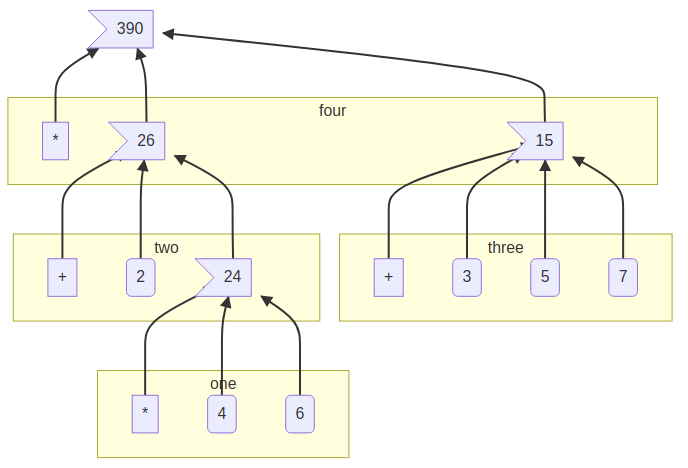
\includegraphics[width=.9\linewidth]{1/fig/t_1-1-3.png}
\end{center}

\subsection{1.1.4: Compound Procedures}
\label{sec:org2268b6e}
We have identified the following in Lisp:
\begin{itemize}
\item primitive data are numbers, primitive procedures are arithmetic operations
\item Operations can be combined by nesting combinations
\item Data and procedures can be abstracted by variable \& procedure definitions
\end{itemize}

Procedure definitions give a name to a compound procedure.
\begin{minted}[breaklines=true,breakanywhere=true,linenos=true]{scheme}
(define (square x) (* x x)) ; to square something, multiply it by itself
; now it can be applied or used in other definitions:
(square 4) ; => 16

(define (sum-of-squares x y)
  (+ (square x) (square y)))
(sum-of-squares 3 4) ; => 25
\end{minted}

Note how these compound procedures are used in the same way as primitive
procedures.

\subsection{1.1.5: The Substitution Model for Procedure Application}
\label{sec:orgf4305a5}
To understand how the interpreter works, imagine it substituting the procedure
calls with the bodies of the procedure and its arguments.

\begin{minted}[breaklines=true,breakanywhere=true,linenos=true]{scheme}
(* (square 3) (square 4))
; has the same results as
(* (* 3 3) (* 3 3))
\end{minted}

This way of understanding procedure application is called the \textbf{substitution
model}. This model is to help you understand procedure substitution, and is
usually not how the interpreter actually works. This book will progress through
more intricate models of interpreters as it goes. This is the natural
progression when learning scientific phenomena, starting with a simple model,
and replace it with more refined models as the phenomena is examined in more
detail.

Evaluations can be done in different orders.

\begin{description}
\item[{\textbf{Applicative order}}] evaluates the operator and operands, and then applies the
\end{description}
resulting procedure to the resulting arguments. In other words, reducing, then
expanding, then reducing.

\begin{description}
\item[{\textbf{Normal order}}] substitutes expressions until it obtains an expression involving
\end{description}
only primitive operators, or until it can't substitute any further, and then
evaluates. This results in expanding the expression completely before doing any
reduction, which results in some repeated evaluations.

For all procedure applications that can be modeled using substitution,
applicative and normal order evaluation produce the same result. Normal order
becomes more complicated once dealing with procedures that can't be modeled by
substitution.

Lisp uses applicative order evaluation because it helps avoid repeated work and
other complications. But normal has its own advantages which will be explored in
Chapter 3 and 4.

\begin{minted}[breaklines=true,breakanywhere=true,linenos=true]{scheme}
; Applicative evaluation
(f 5)
(sum-of-squares (+ a 1) (* a 2))
(sum-of-squares (+ 5 1) (* 5 2))
(sum-of-squares 6 10)
(+ (square x)(square y))
(+ (square 6)(square 10))
(+ (* 6 6)(* 10 10))
(+ 36 100)
136
; Normal evaluation
(f 5)
(sum-of-squares (+ a 1) (* a 2))
(sum-of-squares (+ 5 1) (* 5 2))
(+ (square (+ 5 1)) (square (* 5 2)))
(+ (* (+ 5 1) (+ 5 1)) (* (* 5 2) (* 5 2)))
(+ (* 6 6) (* 10 10))
(+ 36 100)
136
\end{minted}

(Extra-curricular clarification: Normal order delays evaluating arguments until
they're needed by a procedure, which is called lazy evaluation.)

\subsection{1.1.6: Conditional Expressions and Predicates}
\label{sec:org84b28b4}
An important aspect of programming is testing and branching depending on the
results of the test. \texttt{cond} tests \textbf{predicates}, and upon encountering one,
returns a \textbf{consequent}.

\begin{minted}[breaklines=true,breakanywhere=true,linenos=true]{scheme}
(cond
     (predicate1 consequent1)
     ...
     (predicateN consequentN))
\end{minted}

A shorter form of conditional:

\begin{minted}[breaklines=true,breakanywhere=true,linenos=true]{scheme}
(if predicate consequent alternative)
\end{minted}

If \texttt{predicate} is true, \texttt{consequent} is returned. Else, \texttt{alternative} is
returned.

Combining predicates:

\begin{minted}[breaklines=true,breakanywhere=true,linenos=true]{scheme}
(and expression1 ... expressionN)
; if encounters false, stop eval and returns false.
(or expression1 ... expressionN)
; if encounters true, stop eval and return true. Else false.
(not expression)
; true is expression is false, false if expression is true.
\end{minted}

A small clarification:

\begin{minted}[breaklines=true,breakanywhere=true,linenos=true]{scheme}
(define A (* 5 5))
(define (D) (* 5 5))
A ; => 25
D ; => compound procedure D
(D) ; => 25 (result of executing procedure D)
\end{minted}

Special forms bring more nuances into the substitution model mentioned
previously. For example, when evaluating an \texttt{if} expression, you evaluate the
predicate and, depending on the result, either evaluate the \textbf{consequent} or the
\textbf{alternative}. If you were evaluating in a standard manner, the consequent and
alternative would both be evaluated, rendering the \texttt{if} expression ineffective.
\subsection{Exercise 1.1}
\label{sec:org2f81f58}
\subsubsection{Question}
\label{sec:org566bcfe}
\begin{quote}
Below is a sequence of expressions. What is the result printed by the
interpreter in response to each expression? Assume that the sequence is to be
evaluated in the order in which it is presented.
\end{quote}
\subsubsection{Answer}
\label{sec:orgd0e7d1e}
\begin{minted}[breaklines=true,breakanywhere=true,linenos=true]{scheme}
10 ;; 10
(+ 5 3 4) ;; 12
(- 9 1) ;; 8
(/ 6 2) ;; 3
(+ (* 2 4) (- 4 6)) ;; 6
(define a 3) ;; a=3
(define b (+ a 1)) ;; b=4
(+ a b (* a b)) ;; 19
(= a b) ;; false
(if (and (> b a) (< b (* a b)))
    b
    a) ;; 4
(cond ((= a 4) 6)
      ((= b 4) (+ 6 7 a))
      (else 25)) ;; 16
(+ 2 (if (> b a) b a)) ;; 6
(* (cond ((> a b) a)
         ((< a b) b)
         (else -1))
   (+ a 1)) ;; 16
\end{minted}

\subsection{Exercise 1.2}
\label{sec:orga429b03}
\subsubsection{Question}
\label{sec:orge41c737}
\begin{quote}
Translate the following expression into prefix form:
\[
  \frac{5 + 2 + (2 - 3 - (6 + \frac{4}{5})))}
            {3(6 - 2)(2 - 7)}
\]
\end{quote}
\subsubsection{Answer}
\label{sec:org679efe8}
\begin{minted}[breaklines=true,breakanywhere=true,linenos=true]{scheme}
(/ (+ 5 2 (- 2 3 (+ 6 (/ 4 5))))
   (* 3 (- 6 2) (- 2 7)))
\end{minted}

\begin{verbatim}
1/75
\end{verbatim}

\subsection{Exercise 1.3}
\label{sec:org131aad4}
\subsubsection{Question}
\label{sec:org5b611f1}
\begin{quote}
Define a procedure that takes three numbers as arguments and returns the sum of
the squares of the two larger numbers.
\end{quote}
\subsubsection{Answer}
\label{sec:org98eac4f}
\begin{minted}[breaklines=true,breakanywhere=true,linenos=true]{scheme}
<<square>>
(define (sum-square x y)
  (+ (square x) (square y)))
(define (square-2of3 a b c)
  (cond ((and (>= a b) (>= b c)) (sum-square a b))
        ((and (>= a b) (> c b)) (sum-square a c))
        (else (sum-square b c))))
\end{minted}
\begin{minted}[breaklines=true,breakanywhere=true,linenos=true]{scheme}
<<EX1-3>>
<<try-these>>
 (try-these square-2of3 '(7 5 3)
                        '(7 3 5)
                        '(3 5 7))
\end{minted}

\begin{center}
\begin{tabular}{lr}
(7 5 3) & 74\\
(7 3 5) & 74\\
(3 5 7) & 74\\
\end{tabular}
\end{center}

\subsection{Exercise 1.4}
\label{sec:org5b0f382}
\subsubsection{Question}
\label{sec:org6ce70ef}
\begin{quote}
Observe that our model of evaluation allows for combinations whose operators are
compound expressions. Use this observation to describe the behavior of the
following procedure:
\end{quote}

\begin{minted}[breaklines=true,breakanywhere=true,linenos=true]{scheme}
(define (a-plus-abs-b a b)
  ((if (> b 0) + -) a b))
\end{minted}
\subsubsection{Answer}
\label{sec:orgbd70fa7}
This code accepts the variables \texttt{a} and \texttt{b}, and if \texttt{b} is positive, it adds \texttt{a}
and \texttt{b}. However, if \texttt{b} is zero or negative, it subtracts them. This decision
is made by using the \texttt{+} and \texttt{-} procedures as the results of an if expression,
and then evaluating according to the results of that expression. This is in
contrast to a language like Python, which would do something like this:

\begin{minted}[breaklines=true,breakanywhere=true,linenos=true]{python}
if b > 0: a + b
else: a - b
\end{minted}

\subsection{Exercise 1.5}
\label{sec:orgdc041e1}
\subsubsection{Question}
\label{sec:orga3c0be2}
\begin{quote}
Ben Bitdiddle has invented a test to determine whether the interpreter he is
faced with is using applicative-order evaluation or normal-order evaluation. He
defines the following two procedures:
\end{quote}

\begin{minted}[breaklines=true,breakanywhere=true,linenos=true]{scheme}
(define (p) (p))

(define (test x y)
  (if (= x 0)
      0
      y))
\end{minted}
\begin{quote}
Then he evaluates the expression:
\end{quote}

\begin{minted}[breaklines=true,breakanywhere=true,linenos=true]{scheme}
(test 0 (p))
\end{minted}
\begin{quote}


What behavior will Ben observe with an interpreter that uses applicative-order
evaluation? What behavior will he observe with an interpreter that uses
normal-order evaluation? Explain your answer. (Assume that the evaluation rule
for the special form if is the same whether the interpreter is using normal or
applicative order: The predicate expression is evaluated first, and the result
determines whether to evaluate the consequent or the alternative expression.)
\end{quote}

\subsubsection{Answer}
\label{sec:org40709c3}
In either type of language, \mintinline[breaklines=true,breakanywhere=true,linenos=true]{scheme}{(define (p) (p))} is an infinite
loop. However, a normal-order language will encounter the special form, return
\texttt{0}, and never evaluate \mintinline[breaklines=true,breakanywhere=true,linenos=true]{scheme}{(p)}. An applicative-order language evaluates the
arguments to \mintinline[breaklines=true,breakanywhere=true,linenos=true]{scheme}{(test 0 (p))}, thus triggering the infinite
loop.

\subsection{1.1.7: Example: Square Roots by Newton’s Method}
\label{sec:orgd49be79}
Functions in the formal mathematical sense are \textbf{declarative knowledge}, while
procedures like in computer science are \textbf{imperative knowledge}.

Notice that the elements of the language that have been introduced so far are
sufficient for writing any purely numerical program, despite not having
introduced any looping constructs like \texttt{FOR} loops.

\subsection{1.1.8: Procedures as Black-Box Abstractions}
\label{sec:orgacf78a3}
Notice how the \texttt{sqrt} procedure is divided into other procedures, which mirror
the division of the square root problem into sub problems.

A procedure should accomplish an identifiable task, and be ready to be used as a
module in defining other procedures. This lets the programmer know how to use
the procedure while not needing to know the details of how it works.

Suppressing these details are particularly helpful:
\begin{description}
\item[{Local names.}] A procedure user shouldn't need to know a procedure's choices of
variable names. A formal parameter of a procedure whose name is irrelevant is
called a \textbf{bound variable}. A procedure definition \textbf{binds} its parameters. A
\textbf{free variable} isn't bound. The set of expressions in which a binding defines
a name is the \textbf{scope} of that name.
\item[{Internal definitions and block structure.}] By nesting relevant definitions
inside other procedures, you hide them from the global namespace. This nesting
is called \textbf{block structure}. Nesting these definitions also allows relevant
variables to be shared across procedures, which is called \textbf{lexical scoping}.
\end{description}
\subsection{Exercise 1.6}
\label{sec:orgeeb2829}
\subsubsection{Text code}
\label{sec:org6980f9e}
\begin{minted}[breaklines=true,breakanywhere=true,linenos=true]{scheme}
(define (abs x)
  (if (< x 0)
      (- x)
      x))
\end{minted}
\begin{minted}[breaklines=true,breakanywhere=true,linenos=true]{scheme}
(define (average x y)
  (/ (+ x y) 2))
\end{minted}
\begin{minted}[breaklines=true,breakanywhere=true,linenos=true]{scheme}
<<average>>
(define (improve guess x)
  (average guess (/ x guess)))

<<square>>
<<abs>>
(define (good-enough? guess x)
  (< (abs (- (square guess) x)) 0.001))

(define (sqrt-iter guess x)
  (if (good-enough? guess x)
      guess
      (sqrt-iter (improve guess x) x)))

(define (sqrt x)
  (sqrt-iter 1.0 x))
\end{minted}

\subsubsection{Question}
\label{sec:org5bc54e3}
\begin{quote}
Alyssa P. Hacker doesn’t see why \texttt{if} needs to be provided as a
special form. “Why can’t I just define it as an ordinary procedure in terms of
cond?” she asks. Alyssa’s friend Eva Lu Ator claims this can indeed be done, and
she defines a new version of \texttt{if}:
\end{quote}

\begin{minted}[breaklines=true,breakanywhere=true,linenos=true]{scheme}
(define (new-if predicate
                then-clause
                else-clause)
  (cond (predicate then-clause)
        (else else-clause)))
\end{minted}
\begin{quote}
Eva demonstrates the program for Alyssa:
\end{quote}

\begin{minted}[breaklines=true,breakanywhere=true,linenos=true]{scheme}
(new-if (= 2 3) 0 5)
;; => 5

(new-if (= 1 1) 0 5)
;; => 0
\end{minted}

\begin{quote}
Delighted, Alyssa uses new-if to rewrite the square-root program:
\end{quote}

\begin{minted}[breaklines=true,breakanywhere=true,linenos=true]{scheme}
(define (sqrt-iter guess x)
  (new-if (good-enough? guess x)
          guess
          (sqrt-iter (improve guess x) x)))
\end{minted}

\begin{quote}
What happens when Alyssa attempts to use this to compute square roots? Explain.
\end{quote}

\subsubsection{Answer}
\label{sec:org8a8ac3d}
Using Alyssa's \texttt{new-if} leads to an infinite loop because the recursive call to
\texttt{sqrt-iter} is evaluated before the actual call to \texttt{new-if}. This is because
\texttt{if} and \texttt{cond} are special forms that change the way evaluation is handled;
whichever branch is chosen leaves the other branches unevaluated.

\subsection{Exercise 1.7}
\label{sec:org4999f97}
\subsubsection{Text}
\label{sec:orgef75d40}
\begin{minted}[breaklines=true,breakanywhere=true,linenos=true]{scheme}
(define (mean-square x y)
  (average (square x) (square y)))
\end{minted}
\subsubsection{Question}
\label{sec:orgcebafdf}
\begin{quote}
The \texttt{good-enough?} test used in computing square roots will not be very effective
for finding the square roots of very small numbers. Also, in real computers,
arithmetic operations are almost always performed with limited precision. This
makes our test inadequate for very large numbers. Explain these statements, with
examples showing how the test fails for small and large numbers. An alternative
strategy for implementing \texttt{good-enough?} is to watch how guess changes from one
iteration to the next and to stop when the change is a very small fraction of
the guess. Design a square-root procedure that uses this kind of end test. Does
this work better for small and large numbers?
\end{quote}
\subsubsection{Diary}
\label{sec:org2b886f1}
\begin{enumerate}
\item Solving
\label{sec:orga61ab79}
My original answer was this, which compares the previous iteration until the new
and old are within an arbitrary \(dx\).

\begin{minted}[breaklines=true,breakanywhere=true,linenos=true]{scheme}
<<txt-sqrt>>
(define (inferior-good-enough? guess lastguess)
  (<=
   (abs (-
         (/ lastguess guess)
         1))
   0.0000000000001)) ; dx
(define (new-sqrt-iter guess x lastguess) ;; Memory of previous value
  (if (inferior-good-enough? guess lastguess)
      guess
      (new-sqrt-iter (improve guess x) x guess)))
(define (new-sqrt x)
  (new-sqrt-iter 1.0 x 0))
\end{minted}

This solution can correctly find small and large numbers:
\begin{minted}[breaklines=true,breakanywhere=true,linenos=true]{scheme}
<<inferior-good-enough>>
(new-sqrt 10000000000000)
\end{minted}

\begin{verbatim}
3162277.6601683795
\end{verbatim}

\begin{minted}[breaklines=true,breakanywhere=true,linenos=true]{scheme}
<<try-these>>
<<inferior-good-enough>>
(try-these new-sqrt '(0.01 0.0001 0.000001 0.00000001 0.0000000001))
\end{minted}

\begin{center}
\begin{tabular}{rr}
0.01 & 0.1\\
0.0001 & 0.01\\
1e-06 & 0.001\\
1e-08 & 9.999999999999999e-05\\
1e-10 & 9.999999999999999e-06\\
\end{tabular}
\end{center}


However, I found this solution online that isn't just simpler but automatically
reaches the precision limit of the system:

\begin{minted}[breaklines=true,breakanywhere=true,linenos=true]{scheme}
<<txt-sqrt>>
(define (best-good-enough? guess x)
   (= (improve guess x) guess))
\end{minted}

\item Imroving (sqrt) by avoiding extra (improve) call
\label{sec:org18dd839}
\begin{enumerate}
\item Non-optimized
\label{sec:orga9a189a}
\begin{minted}[breaklines=true,breakanywhere=true,linenos=true]{scheme}
(use-modules (ice-9 format))
(load "../mattbench.scm")
(define (average x y)
  (/ (+ x y) 2))
(define (improve guess x)
  (average guess (/ x guess)))
(define (good-enough? guess x)
   (= (improve guess x) guess)) ;; improve call 1
(define (sqrt-iter guess x)
  (if (good-enough? guess x)
      guess
      (sqrt-iter (improve guess x) x))) ;; call 2
(define (sqrt x)
  (sqrt-iter 1.0 x))
(newline)
(display (mattbench (λ() (sqrt 69420)) 400000000))
(newline)
;; 4731.30 <- Benchmark results
\end{minted}

\item Optimized
\label{sec:org80df257}
\begin{minted}[breaklines=true,breakanywhere=true,linenos=true]{scheme}
(use-modules (ice-9 format))
(load "../mattbench.scm")
(define (average x y)
  (/ (+ x y) 2))
(define (improve guess x)
  (average guess (/ x guess)))
(define (good-enough? guess nextguess x)
  (= nextguess guess))
(define (sqrt-iter guess x)
  (let ((nextguess (improve guess x)))
    (if (good-enough? guess nextguess x)
        guess
        (sqrt-iter nextguess x))))
(define (sqrt x)
  (sqrt-iter 1.0 x))
(newline)
(display (mattbench (λ() (sqrt 69420)) 400000000))
(newline)
\end{minted}
\item Benchmark results
\label{sec:org1a31d1f}

\begin{center}
\begin{tabular}{lr}
Unoptimized & 4731.30\\
Optimized & 2518.44\\
\end{tabular}
\end{center}
\end{enumerate}
\end{enumerate}

\subsubsection{Answer}
\label{sec:orgbee417f}
The current method has decreasing accuracy with smaller numbers. Notice the
steady divergence from correct answers here (should be decreasing powers of
0.1):
\begin{minted}[breaklines=true,breakanywhere=true,linenos=true]{scheme}
<<txt-sqrt>>
<<try-these>>
(try-these sqrt 0.01 0.0001 0.000001 0.00000001 0.0000000001)
\end{minted}

\begin{center}
\begin{tabular}{rr}
0.01 & 0.10032578510960605\\
0.0001 & 0.03230844833048122\\
1e-06 & 0.031260655525445276\\
1e-08 & 0.03125010656242753\\
1e-10 & 0.03125000106562499\\
\end{tabular}
\end{center}

And for larger numbers, an infinite loop will eventually be reached. \(10^{12}\)
can resolve, but \(10^{13}\) cannot.

\begin{minted}[breaklines=true,breakanywhere=true,linenos=true]{scheme}
<<txt-sqrt>>
(sqrt 1000000000000)
\end{minted}

\begin{verbatim}
1000000.0
\end{verbatim}

So, my definition of \texttt{sqrt}:
\begin{minted}[breaklines=true,breakanywhere=true,linenos=true]{scheme}
<<average>>
(define (improve guess x)
  (average guess (/ x guess)))
(define (good-enough? guess x)
   (= (improve guess x) guess))
(define (sqrt-iter guess x)
  (if (good-enough? guess x)
      guess
      (sqrt-iter (improve guess x) x)))
(define (sqrt x)
  (sqrt-iter 1.0 x))
\end{minted}
\begin{minted}[breaklines=true,breakanywhere=true,linenos=true]{scheme}
<<try-these>>
<<sqrt>>
(try-these sqrt '(0.01 0.0001 0.000001 0.00000001 0.0000000001))
\end{minted}

\begin{center}
\begin{tabular}{rr}
0.01 & 0.1\\
0.0001 & 0.01\\
1e-06 & 0.001\\
1e-08 & 9.999999999999999e-05\\
1e-10 & 9.999999999999999e-06\\
\end{tabular}
\end{center}

\subsection{Exercise 1.8}
\label{sec:orga58aa19}
\subsubsection{Question}
\label{sec:orga4a2e18}
\begin{quote}
Newton’s method for cube roots is based on the fact that if y is an
approximation to the cube root of x, then a better approximation is given by the
value:
\begin{equation}
\frac{\frac{x}{y^2} + 2y}{3}
\end{equation}
Use this formula to implement a cube-root procedure analogous to the square-root
procedure. (In 1.3.4 we will see how to implement Newton’s method in general as
an abstraction of these square-root and cube-root procedures.)
\end{quote}
\subsubsection{Diary}
\label{sec:orgf87998e}
My first attempt works, but needs an arbitrary limit to stop infinite loops:
\begin{minted}[breaklines=true,breakanywhere=true,linenos=true]{scheme}
<<square>>
<<try-these>>
(define (cb-good-enough? guess x)
  (= (cb-improve guess x) guess))
(define (cb-improve guess x)
  (/
   (+
    (/ x (square guess))
    (* guess 2))
   3))
(define (cbrt-iter guess x counter)
  (if (or (cb-good-enough? guess x) (> counter 100))
      guess
      (begin
        (cbrt-iter (cb-improve guess x) x (+ 1 counter)))))
(define (cbrt x)
  (cbrt-iter 1.0 x 0))

(try-these cbrt 7 32 56 100)
\end{minted}

\begin{center}
\begin{tabular}{rr}
7 & 1.912931182772389\\
32 & 3.174802103936399\\
56 & 3.825862365544778\\
100 & 4.641588833612779\\
\end{tabular}
\end{center}

However, this will hang on an infinite loop when trying to run \mintinline[breaklines=true,breakanywhere=true,linenos=true]{scheme}{(cbrt 100)}. I speculate it's a floating point precision issue with the ``improve''
algorithm. So to avoid it I'll just keep track of the last guess and stop
improving when there's no more change occurring. Also while researching I
discovered that (again due to floating point) \mintinline[breaklines=true,breakanywhere=true,linenos=true]{scheme}{(cbrt -2)} loops
forever unless you initialize your guess with a slightly different value, so
let's do 1.1 instead.
\subsubsection{Answer}
\label{sec:org1025203}
\begin{minted}[breaklines=true,breakanywhere=true,linenos=true]{scheme}
<<square>>
(define (cb-good-enough? nextguess guess lastguess x)
  (or (= nextguess guess)
      (= nextguess lastguess)))
(define (cb-improve guess x)
  (/
   (+
    (/ x (square guess))
    (* guess 2))
   3))
(define (cbrt-iter guess lastguess x)
  (define nextguess (cb-improve guess x))
  (if (cb-good-enough? nextguess guess lastguess x)
      nextguess
      (cbrt-iter nextguess guess x)))
(define (cbrt x)
  (cbrt-iter 1.1 9999 x))
\end{minted}
\begin{minted}[breaklines=true,breakanywhere=true,linenos=true]{scheme}
<<cbrt>>
<<try-these>>
(try-these cbrt 7 32 56 100 -2)
\end{minted}

\begin{center}
\begin{tabular}{rr}
7 & 1.912931182772389\\
32 & 3.174802103936399\\
56 & 3.825862365544778\\
100 & 4.641588833612779\\
-2 & -1.2599210498948732\\
\end{tabular}
\end{center}

\subsection{1.2: Procedures and the Processes They Generate}
\label{sec:org36d1148}
Procedures define the \textbf{local evolution} of processes. We would like to be able
to make statements about the \textbf{global} behavior of a process.

\subsection{1.2.1: Linear Recursion and Iteration}
\label{sec:org1d29fed}
Consider these two procedures for obtaining factorials:

\begin{minted}[breaklines=true,breakanywhere=true,linenos=true]{scheme}
(define (factorial-recursion n)
  (if (= n 1)
      1
      (* n 
         (factorial-recursion (- n 1)))))

(define (factorial-iteration n)
  (define (fact-iter product counter max-count)
      (if (> counter max-count)
          product
          (fact-iter
                    (* counter product)
                    (+ counter 1)
                    max-count)))
  
  (fact-iter 1 1 n))
\end{minted}

These two procedures reach the same answers, but form very different processes.
The \texttt{factorial-recursion} version takes more computational \textbf{time} and \textbf{space} to
evaluate, by building up a chain of deferred operations. This is a \textbf{recursive
process}. As the number of steps needed to operate, and the amount of info
needed to keep track of these operations, both grow linearly with \(n\), this is
a \textbf{linear recursive process}.

The second version forms an \textbf{iterative process}. Its state can be summarized
with a fixed number of state variables. The number of steps required grow
linearly with \(n\), so this is a \textbf{linear iterative process}.

\begin{description}
\item[{recursive procedure}] is a procedure whose definition refers to itself.
\item[{recursive process}] is a process that evolves recursively.
\end{description}

So \texttt{fact-iter} is a recursive \emph{procedure} that generates an iterative \emph{process}.

Many implementations of programming languages interpret all recursive procedures
in a way that consume memory that grows with the number of procedure calls, even
when the process is essentially iterative. These languages instead use looping
constructs such as \texttt{do}, \texttt{repeat}, \texttt{for}, etc. Implementations that execute
iterative processes in constant space, even if the procedure is recursive, are
\textbf{tail-recursive}.
\subsection{Exercise 1.9}
\label{sec:orgd7431e6}
\subsubsection{Question}
\label{sec:org558fd0c}
\begin{quote}
Each of the following two procedures defines a method for adding two positive
integers in terms of the procedures inc, which increments its argument by 1, and
dec, which decrements its argument by 1.
\end{quote}

\begin{minted}[breaklines=true,breakanywhere=true,linenos=true]{scheme}
(define (+ a b)
  (if (= a 0)
      b
      (inc (+ (dec a) b))))

(define (+ a b)
  (if (= a 0)
      b
      (+ (dec a) (inc b))))
\end{minted}

\begin{quote}
Using the substitution model, illustrate the process generated by each procedure
in evaluating \mintinline[breaklines=true,breakanywhere=true,linenos=true]{scheme}{(+ 4 5)}. Are these processes iterative or recursive?
\end{quote}
\subsubsection{Answer}
\label{sec:orgc083090}
The first procedure is recursive, while the second is iterative though
tail-recursion.
\begin{enumerate}
\item recursive procedure
\label{sec:org7abc951}
\begin{minted}[breaklines=true,breakanywhere=true,linenos=true]{scheme}
(+ 4 5)
(inc (+ 3 5))
(inc (inc (+ 2 5)))
(inc (inc (inc (+ 1 5))))
(inc (inc (inc (inc (+ 0 5)))))
(inc (inc (inc (inc 5))))
(inc (inc (inc 6)))
(inc (inc 7))
(inc 8)
9
\end{minted}

\item iterative procedure
\label{sec:org1b47e70}
\begin{minted}[breaklines=true,breakanywhere=true,linenos=true]{scheme}
(+ 4 5)
(+ 3 6)
(+ 2 7)
(+ 1 8)
(+ 0 9)
9
\end{minted}
\end{enumerate}

\subsection{Exercise 1.10}
\label{sec:orga37fd9d}
\subsubsection{Question}
\label{sec:org6f12b4f}
\begin{quote}
The following procedure computes a mathematical function called Ackermann’s
function.
\end{quote}
\begin{minted}[breaklines=true,breakanywhere=true,linenos=true]{scheme}
(define (A x y)
  (cond ((= y 0) 0)
        ((= x 0) (* 2 y))
        ((= y 1) 2)
        (else (A (- x 1)
                 (A x (- y 1))))))
\end{minted}

\begin{quote}
What are the values of the following expressions?
\end{quote}

\begin{minted}[breaklines=true,breakanywhere=true,linenos=true]{scheme}
(A 1 10)
(A 2 4)
(A 3 3)
\end{minted}
\begin{center}
\begin{tabular}{lr}
(1 10) & 1024\\
(2 4) & 65536\\
(3 3) & 65536\\
\end{tabular}
\end{center}

\begin{minted}[breaklines=true,breakanywhere=true,linenos=true]{scheme}
<<ackermann>>
(define (f n) (A 0 n))
(define (g n) (A 1 n))
(define (h n) (A 2 n))
(define (k n) (* 5 n n))
\end{minted}

\begin{quote}
Give concise mathematical definitions for the functions computed by the
procedures \texttt{f}, \texttt{g}, and \texttt{h} for positive integer values of \(n\). For example,
\mintinline[breaklines=true,breakanywhere=true,linenos=true]{scheme}{(k n)} computes \(5n^2\).
\end{quote}

\subsubsection{Answer}
\label{sec:orga86c9f1}
\begin{enumerate}
\item \texttt{f}
\label{sec:orgffd519a}

\begin{minted}[breaklines=true,breakanywhere=true,linenos=true]{scheme}
<<try-these>>
<<EX1-10-defs>>
(try-these f 1 2 3 10 15 20)
\end{minted}

\begin{center}
\begin{tabular}{rr}
1 & 2\\
2 & 4\\
3 & 6\\
10 & 20\\
15 & 30\\
20 & 40\\
\end{tabular}
\end{center}

\[
f(n)=2n
\]
\item \texttt{g}
\label{sec:org7145bb1}

\begin{minted}[breaklines=true,breakanywhere=true,linenos=true]{scheme}
<<try-these>>
<<EX1-10-defs>>
(try-these g 1 2 3 4 5 6 7 8)
\end{minted}

\begin{center}
\begin{tabular}{rr}
1 & 2\\
2 & 4\\
3 & 8\\
4 & 16\\
5 & 32\\
6 & 64\\
7 & 128\\
8 & 256\\
\end{tabular}
\end{center}

\[
g(n)=2^n
\]

\item \texttt{h}
\label{sec:org819c313}

\begin{minted}[breaklines=true,breakanywhere=true,linenos=true]{scheme}
<<try-these>>
<<EX1-10-defs>>
(try-these h 1 2 3 4)
\end{minted}

\begin{center}
\begin{tabular}{rr}
1 & 2\\
2 & 4\\
3 & 16\\
4 & 65536\\
\end{tabular}
\end{center}

It took a while to figure this one out, just because I didn't know the term.
This is repeated exponentiation. This operation is to exponentiation, what
exponentiation is to multiplication. It's called either \emph{tetration} or \emph{hyper-4}
and has no formal notation, but two common ways would be these:

\[
h(n)=2 \uparrow\uparrow n
\]
\[
h(n)={}^{n}2
\]
\end{enumerate}

\subsection{1.2.2: Tree Recursion}
\label{sec:org5de318b}
Consider a recursive procedure for computing Fibonacci numbers:

\begin{minted}[breaklines=true,breakanywhere=true,linenos=true]{scheme}
(define (fib n)
  (cond ((= n 0) 0)
        ((= n 1) 1)
        (else (+ (fib (- n 1))
                 (fib (- n 2))))))
\end{minted}

The resulting process splits into two with every iteration, creating a tree of
computations, many of which are duplicates of previous computations. This kind
of pattern is called \textbf{tree-recursion}. However, this one is quite inefficient.
The time and space required grows exponentially with the number of iterations
requested.

Instead, it makes much more sense to start from \texttt{Fib(1) \textasciitilde{} 1} and \texttt{Fib(0) \textasciitilde{} 0}
and iterate upwards to the desired value. This only requires a linear number of
steps relative to the input.

\begin{minted}[breaklines=true,breakanywhere=true,linenos=true]{scheme}
(define (fib n)
  (fib-iter 1 0 n))
(define (fib-iter a b count)
  (if (= count 0) b (fib-iter (+ a b) a (- count 1))))
\end{minted}

However, notice that the inefficient tree-recursive version is a fairly
straightforward translation of the Fibonacci sequence's definition, while the
iterative version required redefining the process as an iteration with three
variables.

\subsubsection{Example: Counting change}
\label{sec:orgc11094b}
I should come back and try to make the ``better algorithm'' suggested.

\subsection{Exercise 1.11}
\label{sec:org4772088}
\subsubsection{Question}
\label{sec:orgf192ec0}
\begin{quote}
A function \(f\) is defined by the rule that:
\[
f(n)=n \text{ if } n<3
\]
\[
\text{ and }
\]
\[
f(n)=f(n-1)+2f(n-2)+3f(n-3) \text{ if } n \geq 3
\]

Write a procedure that computes \(f\) by means of a recursive process. Write a
procedure that computes \(f\) by means of an iterative process.
\end{quote}
\subsubsection{Answer}
\label{sec:orga8a02e8}
\begin{enumerate}
\item Recursive
\label{sec:org51b96ca}
\begin{minted}[breaklines=true,breakanywhere=true,linenos=true]{scheme}
(define (fr n)
  (if (< n 3)
      n
      (+      (fr (- n 1))
         (* 2 (fr (- n 2)))
         (* 3 (fr (- n 3))))))
\end{minted}

\begin{minted}[breaklines=true,breakanywhere=true,linenos=true]{scheme}
<<try-these>>
<<EX1-11-fr>>
(try-these fr 1 3 5 10)
\end{minted}

\begin{center}
\begin{tabular}{rr}
1 & 1\\
3 & 4\\
5 & 25\\
10 & 1892\\
\end{tabular}
\end{center}

\item Iterative
\label{sec:orgbe22ca4}
\begin{enumerate}
\item Attempt 1
\label{sec:org080d54c}
\begin{minted}[breaklines=true,breakanywhere=true,linenos=true]{scheme}
;; This seems like it could be better
(define (fi n)
  (define (formula l)
    (let ((a (car l))
           (b (cadr l))
           (c (caddr l)))
      (+ a
         (* 2 b)
         (* 3 c))))
  (define (iter l i)
    (if (= i n)
        (car l)
        (iter (cons (formula l) l)
              (+ 1 i))))
  (if (< n 3)
      n
      (iter '(2 1 0) 2)))
\end{minted}

\begin{minted}[breaklines=true,breakanywhere=true,linenos=true]{scheme}
<<try-these>>
<<EX1-11-fi>>
(try-these fi 1 3 5 10)
\end{minted}

\begin{center}
\begin{tabular}{rr}
1 & 1\\
3 & 4\\
5 & 25\\
10 & 1892\\
\end{tabular}
\end{center}

It works but it seems wasteful.

\item Attempt 2
\label{sec:org1bf3086}
\begin{minted}[breaklines=true,breakanywhere=true,linenos=true]{scheme}
(define (fi2 n)
  (define (formula a b c)
      (+ a
         (* 2 b)
         (* 3 c)))
  (define (iter a b c i)
    (if (= i n)
        a
        (iter (formula a b c)
              a
              b
              (+ 1 i))))
  (if (< n 3)
      n
      (iter 2 1 0 2)))
\end{minted}

\begin{minted}[breaklines=true,breakanywhere=true,linenos=true]{scheme}
<<try-these>>
<<EX1-11-fi2>>
(try-these fi2 1 3 5 10)
\end{minted}

\begin{center}
\begin{tabular}{rr}
1 & 1\\
3 & 4\\
5 & 25\\
10 & 1892\\
\end{tabular}
\end{center}

I like that better.
\end{enumerate}
\end{enumerate}

\subsection{Exercise 1.12}
\label{sec:org1d2c4e1}
\subsubsection{Question}
\label{sec:orgb5182a4}
\begin{quote}
The following pattern of numbers is called Pascal’s triangle.

\emph{Pretend there's a Pascal's triangle here.}

The numbers at the edge of the triangle are all 1, and each number inside the
triangle is the sum of the two numbers above it. Write a procedure that
computes elements of Pascal’s triangle by means of a recursive process.
\end{quote}
\subsubsection{Answer}
\label{sec:orgd5d7fd1}
I guess I'll rotate the triangle 45 degrees to make it the top-left corner of an
infinite spreadsheet.

\begin{minted}[breaklines=true,breakanywhere=true,linenos=true]{scheme}
(define (pascal x y)
  (if (or (= x 0)
          (= y 0))
      1
      (+ (pascal (- x 1) y)
         (pascal x (- y 1)))))
\end{minted}

\begin{minted}[breaklines=true,breakanywhere=true,linenos=true]{scheme}
<<try-these>>
<<pascal-rec>>
(let ((l (iota 8)))
  (map (λ (row)
         (map (λ (xy)
                (apply pascal xy))
              row))
       (map (λ (x)
              (map (λ (y)
                     (list x y))
                   l))
            l)))
\end{minted}

\begin{center}
\begin{tabular}{rrrrrrrr}
1 & 1 & 1 & 1 & 1 & 1 & 1 & 1\\
1 & 2 & 3 & 4 & 5 & 6 & 7 & 8\\
1 & 3 & 6 & 10 & 15 & 21 & 28 & 36\\
1 & 4 & 10 & 20 & 35 & 56 & 84 & 120\\
1 & 5 & 15 & 35 & 70 & 126 & 210 & 330\\
1 & 6 & 21 & 56 & 126 & 252 & 462 & 792\\
1 & 7 & 28 & 84 & 210 & 462 & 924 & 1716\\
1 & 8 & 36 & 120 & 330 & 792 & 1716 & 3432\\
\end{tabular}
\end{center}

The test code was much harder to write than the actual solution.

\subsection{Exercise 1.13}
\label{sec:orgf9a9104}
\subsubsection{Question}
\label{sec:org471881c}
\begin{quote}
Prove that \(\text{Fib}(n)\) is the closest integer to
\(\frac{ϕ^n}{\sqrt{5}}\) where Phi is \(\frac{1 + \sqrt{5}}{2}\). Hint: let
\(Υ = \frac{1 - \sqrt{5}}{2}\). Use induction and the definition of the
Fibonacci numbers to prove that

\[
 \text{Fib}(n) = \frac{ϕ^n - Υ^n}{\sqrt{5}}
\]
\end{quote}

\subsubsection{Answer}
\label{sec:org26f9854}
I don't know how to write a proof yet, but I can make functions to
demonstrate it.

\begin{enumerate}
\item Fibonacci number generator
\label{sec:org559314f}
\begin{minted}[breaklines=true,breakanywhere=true,linenos=true]{scheme}
(define (fib-iter n)
  (define (iter i a b)
    (if (= i n)
        b
    (iter (+ i 1)
          b
          (+ a b))))
  (if (<= n 2)
      1
      (iter 2 1 1)))
\end{minted}
\item Various algorithms relating to the question
\label{sec:org5a38592}
\begin{minted}[breaklines=true,breakanywhere=true,linenos=true]{scheme}
<<sqrt>>
(define sqrt5
  (sqrt 5))
(define phi
  (/ (+ 1 sqrt5) 2))
(define upsilon
  (/ (- 1 sqrt5) 2))
(define (fib-phi n)
  (/ (- (expt phi n)
        (expt upsilon n))
     sqrt5))
\end{minted}
\begin{minted}[breaklines=true,breakanywhere=true,linenos=true]{scheme}
(use-srfis '(1))
<<fib-iter>>
<<fib-phi>>
<<try-these>>

(let* ((vals (drop (iota 21) 10))
       (fibs (map fib-iter vals))
       (approx (map fib-phi vals)))
  (zip vals fibs approx))
\end{minted}

\begin{center}
\begin{tabular}{rrr}
10 & 55 & 54.99999999999999\\
11 & 89 & 89.0\\
12 & 144 & 143.99999999999997\\
13 & 233 & 232.99999999999994\\
14 & 377 & 377.00000000000006\\
15 & 610 & 610.0\\
16 & 987 & 986.9999999999998\\
17 & 1597 & 1596.9999999999998\\
18 & 2584 & 2584.0\\
19 & 4181 & 4181.0\\
20 & 6765 & 6764.999999999999\\
\end{tabular}
\end{center}

You can see they follow closely. Graphing the differences, it's just
an exponential curve at very low values, presumably following the
exponential increase of the Fibonacci sequence itself.
\begin{center}
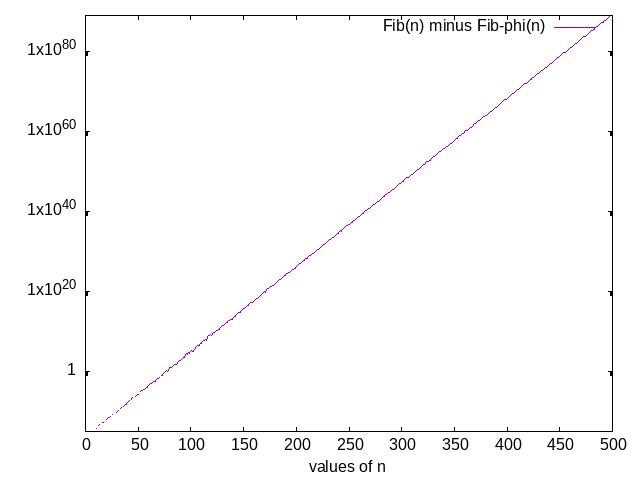
\includegraphics[width=.9\linewidth]{1/fig/1-13.png}
\end{center}
\end{enumerate}

\subsection{1.2.3: Orders of Growth}
\label{sec:org01ab870}
An \textbf{order of growth} gives you a gross measure of the resources required by a
process as its inputs grow larger.

Let \(n\) be a parameter for the size of a problem, and \(R(n)\) be the amount
of resources required for size \(n\). \(R(n)\) has order of growth
\(\Theta(f(n))\)

For example:
\begin{description}
\item[{\(\Theta(1)\)}] is constant, not growing regardless of input size.
\item[{\(\Theta(n)\)}] is growth 1-to-1 proportional to the input size.
\end{description}

Some algorithms we've already seen:
\begin{description}
\item[{Linear recursive}] is time and space \(\Theta(n)\)
\item[{Iterative}] is time \(\Theta(n)\) space \(\Theta(1)\)
\item[{Tree-recursive}] means in general, time is proportional to the number of
nodes, space is proportional to the depth of the tree. In the Fibonacci
algorithm example, \(\Theta(n)\) and time \(\Theta(\Upsilon^{n})\) where
\(\Upsilon\) is the golden ratio \(\frac{1 + \sqrt{5}}{2}\)
\end{description}

Orders of growth are very crude descriptions of process behaviors, but they are
useful in indicating how a process will change with the size of the problem.

\subsection{Exercise 1.14}
\label{sec:org842fdee}
Below is the default version of the count-change function. I'll be aggressively
modifying it in order to get a graph out of it.
\begin{minted}[breaklines=true,breakanywhere=true,linenos=true]{scheme}
(define (count-change amount)
  (cc amount 5))

(define (cc amount kinds-of-coins)
  (cond ((= amount 0) 1)
        ((or (< amount 0)
             (= kinds-of-coins 0))
         0)
        (else
         (+ (cc amount (- kinds-of-coins 1))
            (cc (- amount (first-denomination
                           kinds-of-coins))
                kinds-of-coins)))))

(define (first-denomination kinds-of-coins)
  (cond ((= kinds-of-coins 1) 1)
        ((= kinds-of-coins 2) 5)
        ((= kinds-of-coins 3) 10)
        ((= kinds-of-coins 4) 25)
        ((= kinds-of-coins 5) 50)))
\end{minted}
\subsubsection{Question A}
\label{sec:org18c464e}
\begin{quote}
Draw the tree illustrating the process generated by the count-change procedure
of 1.2.2 in making change for 11 cents.
\end{quote}
\subsubsection{Answer}
\label{sec:org3615a7f}
I want to generate this graph algorithmically.
\begin{minted}[breaklines=true,breakanywhere=true,linenos=true]{scheme}
;; cursed global
(define bubblecounter 0)
;; Returns # of ways change can be made
;; "Helper" for (cc)
(define (count-change amount)
  (display "digraph {\n") ;; start graph
  (cc amount 5 0)
  (display "}\n") ;; end graph
  (set! bubblecounter 0))

;; GraphViz output
;; Derivative: https://stackoverflow.com/a/14806144
(define (cc amount kinds-of-coins oldbubble)
  (let ((recur (lambda (new-amount new-kinds)
                 (begin
                   (display "\"") ;; Source bubble
                   (display `(,oldbubble ,amount ,kinds-of-coins))
                   (display "\"")
                   (display " -> ") ;; arrow pointing from parent to child
                   (display "\"") ;; child bubble
                   (display `(,bubblecounter ,new-amount ,new-kinds))
                   (display "\"")
                   (display "\n")
                   (cc new-amount new-kinds bubblecounter)))))
    (set! bubblecounter (+ bubblecounter 1))
    (cond ((= amount 0) 1)
          ((or (< amount 0) (= kinds-of-coins 0)) 0)
          (else (+
                 (recur amount (- kinds-of-coins 1))
                 (recur (- amount
                           (first-denomination kinds-of-coins))
                        kinds-of-coins))))))

(define (first-denomination kinds-of-coins)
  (cond ((= kinds-of-coins 1) 1)
        ((= kinds-of-coins 2) 5)
        ((= kinds-of-coins 3) 10)
        ((= kinds-of-coins 4) 25)
        ((= kinds-of-coins 5) 50)))
\end{minted}

I'm not going to include the full printout of the \mintinline[breaklines=true,breakanywhere=true,linenos=true]{scheme}{(count-change 11)},
here's an example of what this looks like via \texttt{1}.
\begin{minted}[breaklines=true,breakanywhere=true,linenos=true]{scheme}
<<count-change-graphviz>>
(count-change 1)
\end{minted}

\begin{minted}[breaklines=true,breakanywhere=true,linenos=true]{dot}
digraph {
"(0 1 5)" -> "(1 1 4)"
"(1 1 4)" -> "(2 1 3)"
"(2 1 3)" -> "(3 1 2)"
"(3 1 2)" -> "(4 1 1)"
"(4 1 1)" -> "(5 1 0)"
"(4 1 1)" -> "(6 0 1)"
"(3 1 2)" -> "(7 -4 2)"
"(2 1 3)" -> "(8 -9 3)"
"(1 1 4)" -> "(9 -24 4)"
"(0 1 5)" -> "(10 -49 5)"
}
\end{minted}

\begin{center}
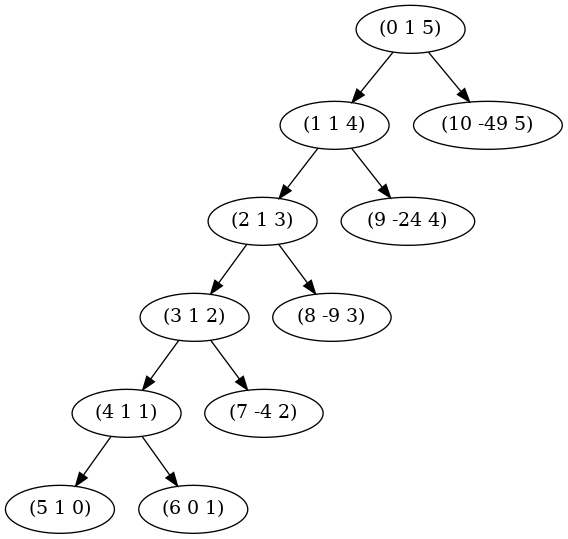
\includegraphics[width=0.6\linewidth]{1/fig/cc-test.png}
\end{center}

So, the graph of \mintinline[breaklines=true,breakanywhere=true,linenos=true]{scheme}{(count-change 11)} is:
\begin{center}
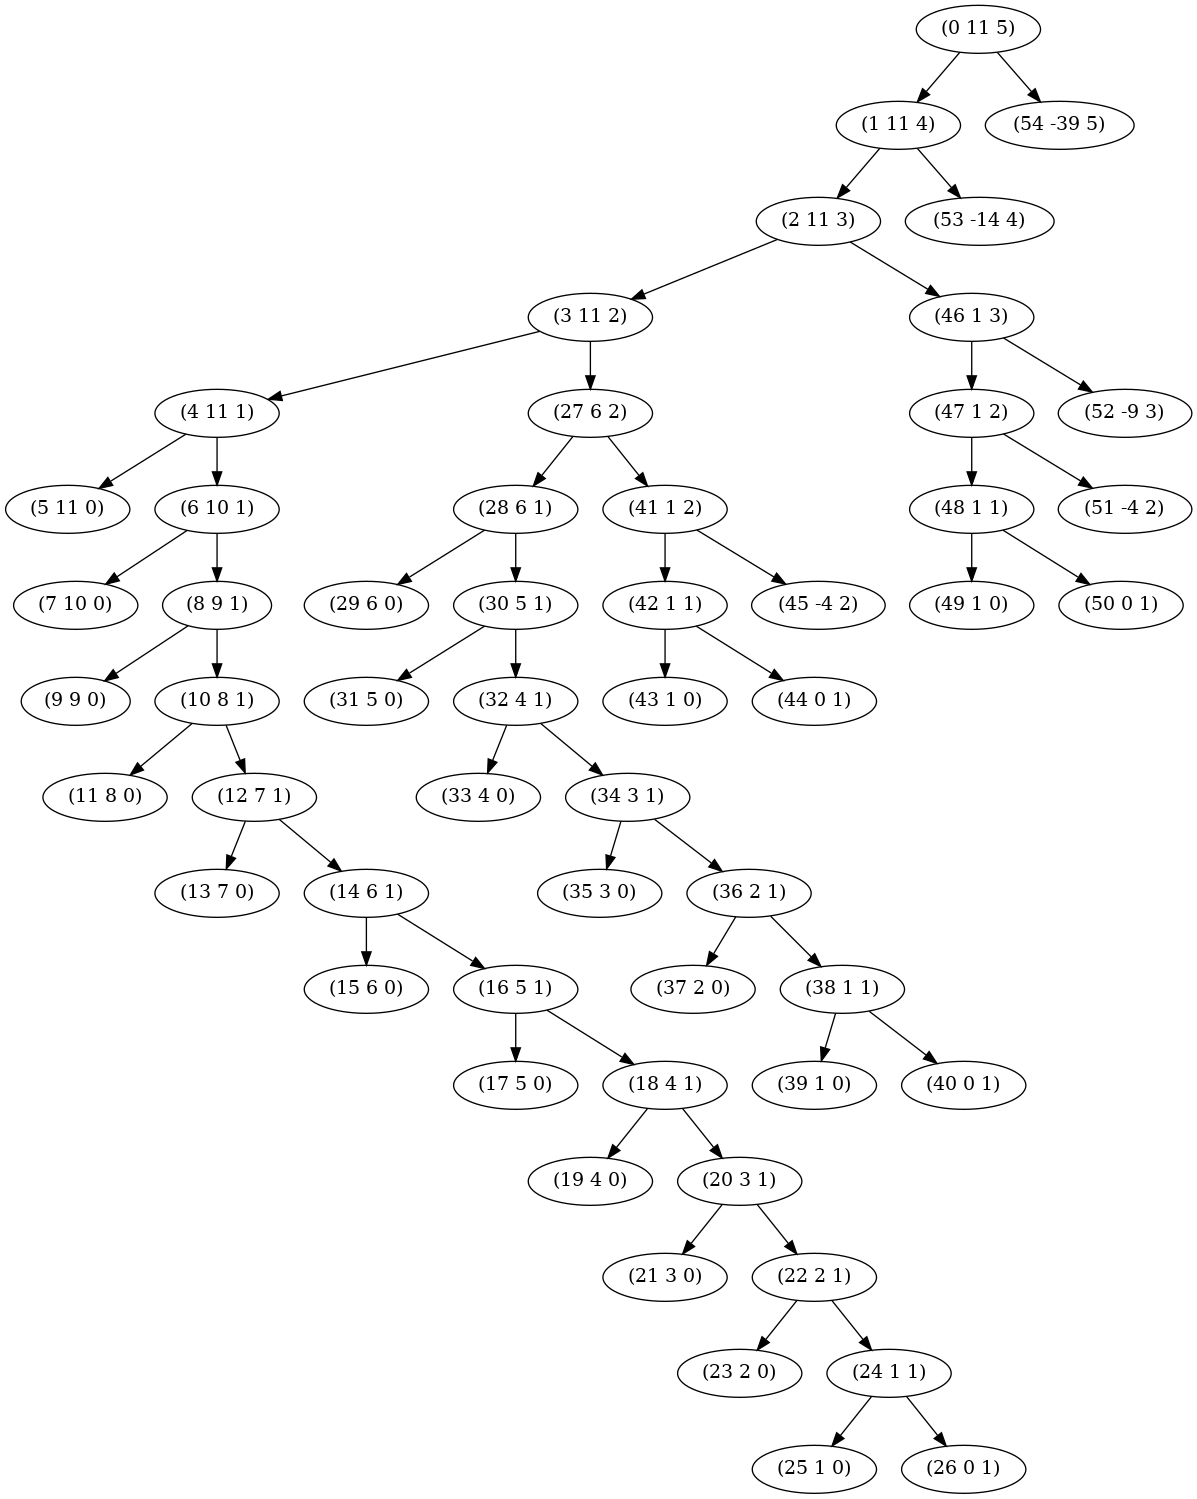
\includegraphics[width=.9\linewidth]{1/fig/cc-11.png}
\end{center}

\subsubsection{Question B}
\label{sec:orgd586b56}
\begin{quote}
What are the orders of growth of the space and number of steps used by this
process as the amount to be changed increases?
\end{quote}

\subsubsection{Answer B}
\label{sec:orga28a07d}
Let's look at this via the number of function calls needed for value \texttt{n}. Instead
of returning an integer, I'll return a pair where \texttt{car} is the number of ways to
count change, and \texttt{cdr} is the number of function calls that have occurred down
that branch of the tree.

\begin{minted}[breaklines=true,breakanywhere=true,linenos=true]{scheme}
(define (count-calls amount)
  (cc-calls amount 5))

(define (cc-calls amount kinds-of-coins)
  (cond ((= amount 0) '(1 . 1))
        ((or (< amount 0)
             (= kinds-of-coins 0))
         '(0 . 1))
        (else
         (let ((a (cc-calls amount (- kinds-of-coins 1)))
               (b (cc-calls (- amount (first-denomination
                                 kinds-of-coins))
                      kinds-of-coins)))
           (cons (+ (car a)
                    (car b))
                 (+ 1
                    (cdr a)
                    (cdr b)))))))

(define (first-denomination kinds-of-coins)
  (cond ((= kinds-of-coins 1) 1)
        ((= kinds-of-coins 2) 5)
        ((= kinds-of-coins 3) 10)
        ((= kinds-of-coins 4) 25)
        ((= kinds-of-coins 5) 50)))
\end{minted}


\begin{minted}[breaklines=true,breakanywhere=true,linenos=true]{scheme}
(use-srfis '(1))
<<cc-calls>>
(let* ((vals (drop (iota 101) 1))
       (mine (map count-calls vals)))
  (zip vals (map car mine) (map cdr mine)))
\end{minted}

\begin{center}
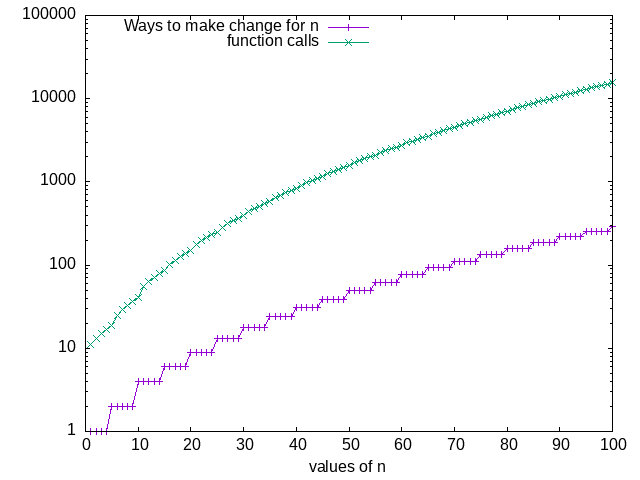
\includegraphics[width=.9\linewidth]{1/fig/cc-100.png}
\end{center}

I believe the space to be \(\Theta(n+d)\) as the function calls count down the
denominations before counting down the change. However I notice most answers
describe \(\Theta(n)\) instead, maybe I'm being overly pedantic and getting the
wrong answer.

My issues came finding the time. The book describes the meaning and properties
of \(\Theta\) notation in \href{http://sarabander.github.io/sicp/html/1\_002e2.xhtml\#g\_t1\_002e2\_002e3}{Section 1.2.3}. However, my lack of formal math
education made realizing the significance of this passage difficult. For one, I
didn't understand that \(k_{1}f(n) \leq R(n) \leq k_{2}f(n)\) means ``you can
find the \(\Theta\) by proving that a graph of the algorithm's resource usage is
bounded by two identical functions multiplied by constants.'' So, the graph of
resource usage for an algorithm with \(\Theta(n^{2})\) will by bounded by lines
of \(n^{2} \times some constant\), the top boundary's constant being larger than
the small boundary. These are arbitrarily chosen constants, you're just proving
that the function behaves the way you think it does.

Overall, finding the \(\Theta\) and \(\Omega\) and \(O\) notations (they are all
different btw!) is about aggressively simplifying to make a very general
statement about the behavior of the algorithm.

I could tell that a ``correct'' way to find the \(\Theta\) would be to make a
formula which describes the algorithm's function calls for given input and
denominations. This is one of the biggest time sinks, although I had a lot of
fun and learned a lot. In the end, with some help from Jach in a Lisp Discord, I
had the following formula:

\[
\sum_{i=1}^{ceil(n / val(d))} T(n - val(d)*i, d)
\]

But I wasn't sure where to go from here. The graphs let me see some interesting
trends, though I didn't get any closer to an answer in the process.

By reading on other websites, I knew that you could find \(\Theta\) by obtaining
a formula for \(R(n)\) and removing constants to end up with a term of interest.
For example, if your algorithm's resource usage is \(\frac{n^{2} + 7n}{5}\),
this demonstrates \(\Theta(n^{2})\). So I know a formula \textbf{without} a \(\sum\)
would give me the answer I wanted. It didn't occur to me that it might be
possible to use calculus to remove the \(\sum\) from the equation. At this point
I knew I was stuck and decided to look up a guide.

After seeing a few solutions that I found somewhat confusing, I landed on \href{https://codology.net/post/sicp-solution-exercise-1-14/}{this
awesome article from Codology.net}. They show how you can remove the summation,
and proposed this equation for count-change with 5 denominations:

\[
T(n,5)=\frac n{50}+1+\sum_{i=0}^{n/50}T(n-50i,1)
\]

Which, when expanded and simplified, demonstrates \(\Theta(n^{5})\) for 5
denominations.

Overall I'm relieved that I wasn't entirely off, given I haven't done math work
like this since college. It's inspired me to restart my remedial math courses, I
don't think I really grasped the nature of math as a tool of empowerment until
now.

\subsection{Exercise 1.15}
\label{sec:org70c3267}
\subsubsection{Question A}
\label{sec:org5e6cbc2}
\begin{quote}
The sine of an angle (specified in radians) can be computed by making use of the
approximation \(\sin x ≈ x\) if \(x\) is sufficiently small, and the
trigonometric identity \(\sin x = 3\sin\frac{x}{3} − 4\sin^3\frac{x}{3}\)
to reduce the size of the argument of sin. (For purposes of this exercise an
angle is considered “sufficiently small” if its magnitude is not greater than
0.1 radians.) These ideas are incorporated in the following procedures:
\end{quote}

\begin{minted}[breaklines=true,breakanywhere=true,linenos=true]{scheme}
(define (cube x) (* x x x))
(define (p x) (- (* 3 x) (* 4 (cube x))))
(define (sine angle)
  (if (not (> (abs angle) 0.1))
      angle
      (p (sine (/ angle 3.0)))))
\end{minted}

\begin{quote}
How many times is the procedure \texttt{p} applied when \mintinline[breaklines=true,breakanywhere=true,linenos=true]{scheme}{(sine 12.15)} is
evaluated?
\end{quote}

\subsubsection{Answer A}
\label{sec:orgca8ab23}

Let's find out!
\begin{minted}[breaklines=true,breakanywhere=true,linenos=true]{scheme}
(define (cube x) (* x x x))
(define (p x) (- (* 3 x) (* 4 (cube x))))
(define (sine angle)
  (if (not (> (abs angle) 0.1))
      (cons angle 0)
      (let ((x (sine (/ angle 3.0))))
        (cons (p (car x)) (+ 1 (cdr x))))))
\end{minted}

\begin{minted}[breaklines=true,breakanywhere=true,linenos=true]{scheme}
<<1-15-p-measure>>
(let ((xy (sine 12.15)))
  (list (car xy) (cdr xy)))
\end{minted}

\begin{center}
\begin{tabular}{rr}
-0.39980345741334 & 5\\
\end{tabular}
\end{center}

\texttt{p} is evaluated 5 times.

\subsubsection{Question B}
\label{sec:orgc22c06b}
\begin{quote}
What is the order of growth in space and number of steps (as a function of \texttt{a})
used by the process generated by the sine procedure when \mintinline[breaklines=true,breakanywhere=true,linenos=true]{scheme}{(sine a)} is
evaluated?
\end{quote}

\subsubsection{Answer B}
\label{sec:org1e43101}
\begin{minted}[breaklines=true,breakanywhere=true,linenos=true]{scheme}
(use-srfis '(1))
<<1-15-p-measure>>
(let* ((vals (iota 300 0.1 0.1))
       (sines (map (λ (i)
                     (cdr (sine i)))
                   vals)))
  (zip vals sines))
\end{minted}
\begin{minted}[breaklines=true,breakanywhere=true,linenos=true]{scheme}
(use-srfis '(1))
<<1-15-p-measure>>
(let* ((vals (iota 10 0.1 0.1))
       (sines (map (λ (i)
                     (cdr (sine i)))
                   vals)))
  (zip vals sines))
\end{minted}

Example output:
\begin{center}
\begin{tabular}{rr}
0.1 & 0\\
0.2 & 1\\
0.30000000000000004 & 2\\
0.4 & 2\\
0.5 & 2\\
0.6 & 2\\
0.7000000000000001 & 2\\
0.8 & 2\\
0.9 & 2\\
1.0 & 3\\
\end{tabular}
\end{center}

\begin{center}
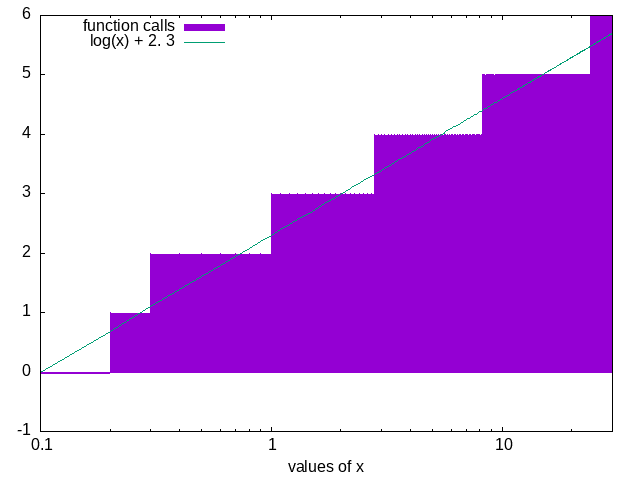
\includegraphics[width=.9\linewidth]{1/fig/1-15-step.png}
\end{center}

This graph shows that the number of times \texttt{sine} will be called is logarithmic.
\begin{itemize}
\item 0.1 to 0.2 are divided once
\item 0.3 to 0.8 are divided twice
\item 0.9 to 2.6 are divided three times
\item 2.7 to 8 are divided four times
\item 8.5 to 23.8 are divided five times
\end{itemize}

Given that the calls to \texttt{p} get stacked recursively, like this:
\begin{minted}[breaklines=true,breakanywhere=true,linenos=true]{scheme}
(sine 12.15)
(p (sine 4.05))
(p (p (sine 1.35)))
(p (p (p (sine 0.45))))
(p (p (p (p (sine 0.15)))))
(p (p (p (p (p (sine 0.05))))))
(p (p (p (p (p 0.05)))))
(p (p (p (p 0.14950000000000002))))
(p (p (p 0.43513455050000005)))
(p (p 0.9758465331678772))
(p -0.7895631144708228)
-0.39980345741334
\end{minted}

So I argue the space and time is \(\Theta(\log(n))\)


We can also prove this for the time by benchmarking the function:

\begin{minted}[breaklines=true,breakanywhere=true,linenos=true]{scheme}
;; This execution takes too long for org-mode, so I'm doing it
;; externally and importing the results
(use-srfis '(1))
(use-modules (ice-9 format))
(load "../../mattbench.scm")
<<1-15-deps>>
(let* ((vals (iota 300 0.1 0.1))
       (times (map (λ (i)
                     (mattbench (λ () (sine i)) 1000000))
                   vals)))
  (with-output-to-file "sine-bench.dat" (λ ()
     (map (λ (x y)
           (format #t "~s~/~s~%" x y))
         vals times))))
\end{minted}

\begin{minted}[breaklines=true,breakanywhere=true,linenos=true]{gnuplot}
reset # helps with various issues in execution
set xtics 0.5
set xlabel 'values of x'
set logscale x
set key top left
set style fill solid 1.00 border
#set style function fillsteps below

f(x) = (log(x) * a) + b
fit f(x) 'Ex15/sine-bench.dat' using 1:2 via a,b

plot 'Ex15/sine-bench.dat' using 1:2 with fillsteps title 'time to execute', \
     'Ex15/sine-bench.dat' using 1:(f($1)) with lines title sprintf('(log(x) * %.2f) + %.2f', a, b)
\end{minted}

\begin{center}
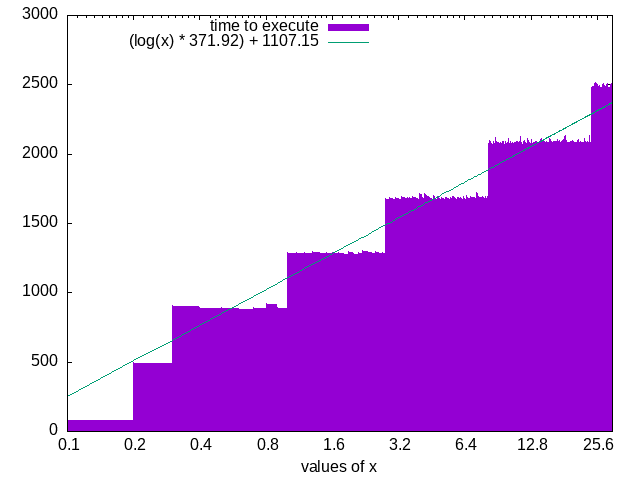
\includegraphics[width=.9\linewidth]{1/fig/1-15-bench.png}
\end{center}

\begin{enumerate}
\item 1.2.4 Exponentiation
\label{sec:orgb7f118e}
Considering a few ways to compute the exponential of a given number.

\begin{minted}[breaklines=true,breakanywhere=true,linenos=true]{scheme}
(define (expt b n)
  (expt-iter b n 1))
(define (expt-iter b counter product)
  (if (= counter 0)
      product
      (expt-iter b (- counter 1) (* b product))))
\end{minted}

This iterative procedure is essentially equivalent to:

\[b^{8} = b \cdot (b \cdot (b \cdot (b \cdot (b \cdot (b \cdot (b \cdot b))))))\]

But note it could be approached faster with squaring:

\[\begin{aligned}b^2 &= b \cdot b\\
b^4 &= b^2\cdot b^2\\
b^8 &= b^4 \cdot b^4\end{aligned}\]
\end{enumerate}

\subsection{Exercise 1.16}
\label{sec:org7a8345f}
\subsubsection{Text}
\label{sec:org3475b45}
\begin{minted}[breaklines=true,breakanywhere=true,linenos=true]{scheme}
(define (expt-rec b n)
  (if (= n 0) 
      1 
      (* b (expt-rec b (- n 1)))))

(define (expt-iter b n) 
  (define (iter counter product)
    (if (= counter 0)
        product
        (iter (- counter 1)
              (* b product))))
  (iter n 1))

(define (fast-expt b n)
  (cond ((= n 0) 
         1)
        ((even? n) 
         (square (fast-expt b (/ n 2))))
        (else 
         (* b (fast-expt b (- n 1))))))
\end{minted}
\subsubsection{Question}
\label{sec:org369d14b}
\begin{quote}
Design a procedure that evolves an iterative exponentiation process that uses
successive squaring and uses a logarithmic number of steps, as does fast-expt.
(Hint: Using the observation that \((b^{n/2})^2=(b^2)^{n/2}\), keep, along with
the exponent \(n\) and the base \(b\), an additional state variable \(a\) , and
define the state transformation in such a way that the product \({ab}^n\) is
unchanged from state to state. At the beginning of the process \(a\) is taken to
be 1, and the answer is given by the value of \(a\) at the end of the process.
In general, the technique of defining an \emph{invariant quantity} that remains
unchanged from state to state is a powerful way to think about the design of
iterative algorithms.)
\end{quote}
\subsubsection{Diary}
\label{sec:org05248ff}
First I made this program which tries to use a false equivalence:
\[ab^2 = (a + 1)b^{n - 1}\]
\begin{minted}[breaklines=true,breakanywhere=true,linenos=true]{scheme}
<<square>>
(define (fast-expt-iter b n)
  (define (iter b n a)
    (format #t "~&|~s~/~/|~s~/~/|~s|~%" b n a)
    (cond ((= n 1) (begin (format #t "~&|~s~/~/|~s~/~/|~s|~%" (* b a) 1 1)
                          (* b a)))
          ((even? n) (iter (square b)
                         (/ n 2)
                         a))
          (else (iter b (- n 1) (+ a 1)))))
  (format #t "|~a~/|~a~/|~a|~%" "base" "power" "variable")
  (format #t "~&|--|--|--|~%")
  (iter b n 1))
\end{minted}

\begin{minted}[breaklines=true,breakanywhere=true,linenos=true]{scheme}
<<fast-expt-iter-fail1>>
<<try-these>>
(fast-expt-iter 2 6)
\end{minted}

Here's what the internal state looks like during \(2^6\) (correct answer is 64):
\begin{center}
\begin{tabular}{rrr}
base & power & variable\\
\hline
2 & 6 & 1\\
4 & 3 & 1\\
4 & 2 & 2\\
16 & 1 & 2\\
32 & 1 & 1\\
\end{tabular}
\end{center}

\subsubsection{Answer}
\label{sec:orgf061e25}
There are two key transforms to a faster algorithm. The first was already shown
in the text:

\[
    ab^n \to a(b^2)^{n/2}
\]

The second which I needed to deduce was this:

\[
    ab^n \to ((a \times b) \times b)^{n - 1}
\]

The solution essentially follows this logic:
\begin{itemize}
\item initialize \(a\) to 1
\item If \(n\) is 1, return \(b * a\)
\item else if \(n\) is even, halve \(n\), square \(b\), and iterate
\item else \(n\) is odd, so subtract 1 from \(n\) and \(a \to a \times b\)
\end{itemize}

\begin{minted}[breaklines=true,breakanywhere=true,linenos=true]{scheme}
<<square>>
(define (fast-expt-iter b n)
  (define (iter b n a)
    (cond ((= n 1) (* b a))
          ((even? n) (iter (square b)
                         (/ n 2)
                         a))
          (else (iter b (- n 1) (* b a)))))
  (iter b n 1))
\end{minted}

\begin{minted}[breaklines=true,breakanywhere=true,linenos=true]{scheme}
<<fast-expt-iter>>
<<try-these>>
(try-these (λ(x) (fast-expt-iter 3 x)) (cdr (iota 11)))
\end{minted}

\begin{center}
\begin{tabular}{rr}
1 & 3\\
2 & 9\\
3 & 27\\
4 & 81\\
5 & 243\\
6 & 729\\
7 & 2187\\
8 & 6561\\
9 & 19683\\
10 & 59049\\
\end{tabular}
\end{center}

\subsection{Exercise 1.17}
\label{sec:org6ce19b0}
\subsubsection{Question}
\label{sec:orge14e929}
\begin{quote}
The exponentiation algorithms in this section are based on performing
exponentiation by means of repeated multiplication. In a similar way, one can
perform integer multiplication by means of repeated addition. The following
multiplication procedure (in which it is assumed that our language can only add,
not multiply) is analogous to the expt procedure:
\end{quote}

\begin{minted}[breaklines=true,breakanywhere=true,linenos=true]{scheme}
(define (* a b)
  (if (= b 0)
      0
      (+ a (* a (- b 1)))))
\end{minted}

\begin{quote}
This algorithm takes a number of steps that is linear in \(b\). Now suppose we
include, together with addition, operations double, which doubles an integer,
and halve, which divides an (even) integer by 2. Using these, design a
multiplication procedure analogous to fast-expt that uses a logarithmic number
of steps.
\end{quote}

\subsubsection{Answer}
\label{sec:org5c12422}
\begin{minted}[breaklines=true,breakanywhere=true,linenos=true]{scheme}
(define (double x)
  (+ x x))
(define (halve x)
  (/ x 2))
(define (fast-mult-rec a b)
  (cond ((= b 0) 0)
        ((even? b)
         (double (fast-mult-rec a (halve b)))) ; This was kind of a stretch to think of.G
         ;(fast-mult (double a) (halve b))) <== My first instinct is iterative
        (else (+ a (fast-mult-rec a (- b 1))))))
\end{minted}

Proof it works:

\begin{minted}[breaklines=true,breakanywhere=true,linenos=true]{scheme}
<<fast-mult-rec>>
<<try-these>>
(try-these (λ(x) (fast-mult-rec 3 x)) (cdr (iota 11)))
\end{minted}

\begin{center}
\begin{tabular}{rr}
1 & 3\\
2 & 6\\
3 & 9\\
4 & 12\\
5 & 15\\
6 & 18\\
7 & 21\\
8 & 24\\
9 & 27\\
10 & 30\\
\end{tabular}
\end{center}

\subsection{Exercise 1.18}
\label{sec:org6b749e3}
\subsubsection{Question}
\label{sec:orgcb8647b}
\begin{quote}
Using the results of \hyperref[sec:org7a8345f]{Exercise 1.16} and \hyperref[sec:org6ce19b0]{Exercise 1.17}, devise a procedure that
generates an iterative process for multiplying two integers in terms of adding,
doubling, and halving and uses a logarithmic number of steps.
\end{quote}
\subsubsection{Diary}
\label{sec:org23b040e}
\begin{enumerate}
\item Comparison benchmarks:
\label{sec:org1a80d9d}

\begin{minted}[breaklines=true,breakanywhere=true,linenos=true]{scheme}
(load "../mattbench.scm")
<<fast-mult-iter>>
<<fast-mult-rec>>
<<print-table>>
(print-table (list (list "fast-mult-rec" "fast-mult-iter")
                   (list (mattbench (λ() (fast-mult-rec 32 32)) 10000000)
                         (mattbench (λ() (fast-mult 32 32)) 10000000)))
             #:colnames #t)
\end{minted}

\begin{center}
\begin{tabular}{rr}
``fast-mult-rec'' & ``fast-mult-iter''\\
\hline
196.89 & 166.35\\
\end{tabular}
\end{center}

So the iterative version takes 0.84 times less to do \(32 \times 32\).
\item Hall of shame
\label{sec:org05e033b}
Some of my \emph{very} incorrect ideas:
\[ab = (a+1)(b-1)\]
\[ab = \big(a+\Big(\frac{a}{2}\Big)(b-1)\big)\]
\[ab+c = \big(a(b-1)+(b+c)\big)\]
\end{enumerate}
\subsubsection{Answer}
\label{sec:orgfab6f90}
\begin{minted}[breaklines=true,breakanywhere=true,linenos=true]{scheme}
(define (double x)
  (+ x x))
(define (halve x)
  (/ x 2))
(define (fast-mult a b)
  (define (iter a b c)
    (cond ((= b 0) 0)
          ((= b 1) (+ a c))
          ((even? b)
           (iter (double a) (halve b) c))
          (else (iter a (- b 1) (+ a c)))))
  (iter a b 0))
\end{minted}
\begin{minted}[breaklines=true,breakanywhere=true,linenos=true]{scheme}
<<fast-mult-iter>>
<<try-these>>
(try-these (λ(x) (fast-mult 3 x)) (cdr (iota 11)))
\end{minted}

\begin{center}
\begin{tabular}{rr}
1 & 3\\
2 & 6\\
3 & 9\\
4 & 12\\
5 & 15\\
6 & 18\\
7 & 21\\
8 & 24\\
9 & 27\\
10 & 30\\
\end{tabular}
\end{center}

\subsection{Exercise 1.19}
\label{sec:org970f052}
\subsubsection{Question}
\label{sec:org89fd361}
\begin{quote}
There is a clever algorithm for computing the Fibonacci numbers in a logarithmic
number of steps. Recall the transformation of the state variables a and b in the
\texttt{fib-iter} process of section 1-2-2:

\[a <- a + b\text{ and }b <- a\]

Call this transformation T, and observe that applying T over and over again n
times, starting with 1 and 0, produces the pair \_Fib\textsubscript{(n + 1)} and \_Fib\textsubscript{(n)}. In
other words, the Fibonacci numbers are produced by applying \(T^n\), the nth
power of the transformation T, starting with the pair (1,0). Now consider T to
be the special case of p = 0 and q = 1 in a family of transformations \(T_{(pq)}\), where \(T_{(pq)}\) transforms the pair (a,b) according to \(a <-
bq + aq + ap\) and \(b <- bp + aq\). Show that if we apply such a
transformation \(T_{(pq)}\) twice, the effect is the same as using a single
transformation \(T_{(p'q')}\) of the same form, and compute p' and q' in terms
of p and q. This gives us an explicit way to square these transformations, and
thus we can compute \(T^n\) using successive squaring, as in the `fast-expt'
procedure. Put this all together to complete the following procedure, which runs
in a logarithmic number of steps:
\end{quote}
\begin{minted}[breaklines=true,breakanywhere=true,linenos=true]{scheme}
(define (fib n)
  (fib-iter 1 0 0 1 n))

(define (fib-iter a b p q count)
  (cond ((= count 0) b)
        ((even? count)
         (fib-iter a
                   b
                   <??>      ; compute p'
                   <??>      ; compute q'
                   (/ count 2)))
        (else (fib-iter (+ (* b q) (* a q) (* a p))
                        (+ (* b p) (* a q))
                        p
                        q
                        (- count 1)))))
\end{minted}

\subsubsection{Diary}
\label{sec:org146eeed}
More succinctly put:

\[
    \text{Fib}_n \begin{cases}
        a \leftarrow a + b\\
        b \leftarrow a
    \end{cases}
\]
\[
    \text{Fib-iter}_{abpq} \begin{cases}
        a \leftarrow bq + aq + ap\\
        b \leftarrow bp + aq
    \end{cases}
\]

\mintinline[breaklines=true,breakanywhere=true,linenos=true]{scheme}{(T)} returns a transformation function based on the two numbers in
the attached list. so \mintinline[breaklines=true,breakanywhere=true,linenos=true]{scheme}{(T 0 1)} returns a fib function.

\begin{minted}[breaklines=true,breakanywhere=true,linenos=true]{scheme}
(define (T p q)
  (λ (a b)
    (cons (+ (* b q) (* a q) (* a p))
          (+ (* b p) (* a q)))))

(define T-fib
  (T 0 1))

;; Repeatedly apply T functions:
(define (Tr f n)
  (Tr-iter f n 0 1))
(define (Tr-iter f n a b)
  (if (= n 0)
      a
      (let ((l (f a b)))
        (Tr-iter f (- n 1) (car l) (cdr l)))))
\end{minted}

\[
    \text{T}_{pq}: a,b\mapsto \begin{cases}
        a \leftarrow bq + aq + ap\\
        b \leftarrow bp + aq
    \end{cases}
\]

\begin{minted}[breaklines=true,breakanywhere=true,linenos=true]{scheme}
<<T-func>>
<<try-these>>
(try-these (λ (x) (Tr (T 0 1) x)) (cdr (iota 11)))
\end{minted}

\begin{center}
\begin{tabular}{rr}
1 & 1\\
2 & 1\\
3 & 2\\
4 & 3\\
5 & 5\\
6 & 8\\
7 & 13\\
8 & 21\\
9 & 34\\
10 & 55\\
\end{tabular}
\end{center}

\subsubsection{Answer}
\label{sec:org8a89915}
\begin{minted}[breaklines=true,breakanywhere=true,linenos=true]{scheme}
(define (fib-rec n)
  (cond ((= n 0) 0)
        ((= n 1) 1)
        (else (+ (fib-rec (- n 1))
                 (fib-rec (- n 2))))))
(define (fib n)
  (fib-iter 1 0 0 1 n))

(define (fib-iter a b p q count)
  (cond ((= count 0) b)
        ((even? count)
         (fib-iter a
                   b
                   (+ (* p p)
                      (* q q))      ; compute p'
                   (+ (* p q)
                      (* q q)
                      (* q p))      ; compute q'
                   (/ count 2)))
        (else (fib-iter (+ (* b q) (* a q) (* a p))
                        (+ (* b p) (* a q))
                        p
                        q
                        (- count 1)))))
\end{minted}

\begin{center}
\begin{tabular}{rrr}
``n'' & ``fib-rec'' & ``fib-iter''\\
\hline
1 & 1 & 1\\
2 & 1 & 1\\
3 & 2 & 2\\
4 & 3 & 3\\
5 & 5 & 5\\
6 & 8 & 8\\
7 & 13 & 13\\
8 & 21 & 21\\
9 & 34 & 34\\
\end{tabular}
\end{center}

\subsection{1.2.5: Greatest Common Divisor}
\label{sec:orgaadd364}
A greatest common divisor (or GCD) for two integers is the largest integer that
divides both of them. A GCD can be quickly found by transforming the problem
like so: \[a \% b = r\]

\[\text{GCD}(a, b) = \text{GCD}(b, r)\]

This eventually produces a pair where the second number is 0. Then, the GCD is
the other number in the pair. This is Euclid's Algorithm.

\[\begin{aligned}\text{GCD}(206,40) &= \text{GCD}(40,6)\\ &=
            \text{GCD}(6,4)\\ &= \text{GCD}(4,2)\\ &~ \text{GCD}(2,0) ~
            2\end{aligned}\]

\begin{quote}
\textbf{Lamé's Theorem:} If Euclid's Algorithm requires \(k\) steps to compute the
 GCD of some pair, then the smaller number in the pair must be greater than or
 equal to the \(k^{th}\)Fibonacci number.
\end{quote}

\subsection{Exercise 1.20}
\label{sec:orge56b07b}
\subsubsection{Text}
\label{sec:org68fba82}
\begin{minted}[breaklines=true,breakanywhere=true,linenos=true]{scheme}
(define (gcd a b)
  (if (= b 0)
      a
      (gcd b (remainder a b))))
\end{minted}
\subsubsection{Question}
\label{sec:orga3b291e}
\begin{quote}
The process that a procedure generates is of course dependent on the rules used
by the interpreter. As an example, consider the iterative \texttt{gcd} procedure given
above. Suppose we were to interpret this procedure using normal-order
evaluation, as discussed in 1.1.5. (The normal-order-evaluation rule for \texttt{if} is
described in Exercise 1.5.) Using the substitution method (for normal order),
illustrate the process generated in evaluating \mintinline[breaklines=true,breakanywhere=true,linenos=true]{scheme}{(gcd 206 40)} and indicate the
remainder operations that are actually performed. How many remainder operations
are actually performed in the normal-order evaluation of \mintinline[breaklines=true,breakanywhere=true,linenos=true]{scheme}{(gcd 206 40)}? In the
applicative-order evaluation?
\end{quote}

\subsubsection{Answer}
\label{sec:org907da71}
I struggled to understand this, but the key here is that normal-order evaluation
causes the unevaluated expressions to be duplicated, meaning they get evaluated
multiple times.

\begin{enumerate}
\item Applicative order
\label{sec:org293b414}
\begin{minted}[breaklines=true,breakanywhere=true,linenos=true]{scheme}
call (gcd 206 40)
(if)
(gcd 40 (remainder 206 40))
eval remainder before call
call (gcd 40 6)
(if)
(gcd 6 (remainder 40 6))
eval remainder before call
call (gcd 6 4)
(if)
(gcd 2 (remainder 4 2))
eval remainder before call
call (gcd 2 0)
(if)
;; => 2
\end{minted}

\begin{minted}[breaklines=true,breakanywhere=true,linenos=true]{scheme}
;; call gcd
(gcd 206 40)

;; eval conditional
(if (= 40 0)
    206
    (gcd 40 (remainder 206 40)))

;; recurse
(gcd 40 (remainder 206 40))

; encounter conditional
(if (= (remainder 206 40) 0)
    40
    (gcd (remainder 206 40)
         (remainder 40 (remainder 206 40))))

; evaluate 1 remainder
(if (= 6 0)
    40
    (gcd (remainder 206 40)
         (remainder 40 (remainder 206 40))))

; recurse
(gcd (remainder 206 40)
     (remainder 40 (remainder 206 40)))

; encounter conditional
(if (= (remainder 40 (remainder 206 40)) 0)
    (remainder 206 40)
    (gcd (remainder 40 (remainder 206 40))
         (remainder (remainder 206 40) (remainder 40 (remainder 206 40)))))

; eval 2 remainder
(if (= 4 0)
    (remainder 206 40)
    (gcd (remainder 40 (remainder 206 40))
         (remainder (remainder 206 40) (remainder 40 (remainder 206 40)))))

; recurse
(gcd (remainder 40 (remainder 206 40))
     (remainder (remainder 206 40) (remainder 40 (remainder 206 40))))

; encounter conditional
(if (= (remainder (remainder 206 40) (remainder 40 (remainder 206 40))) 0)
    (remainder 40 (remainder 206 40))
    (gcd (remainder (remainder 206 40) (remainder 40 (remainder 206 40)))
         (remainder (remainder 40 (remainder 206 40)) (remainder (remainder 206 40) (remainder 40 (remainder 206 40))))))

; eval 4 remainders
(if (= 2 0)
    (remainder 40 (remainder 206 40))
    (gcd (remainder (remainder 206 40) (remainder 40 (remainder 206 40)))
         (remainder (remainder 40 (remainder 206 40)) (remainder (remainder 206 40) (remainder 40 (remainder 206 40))))))

; recurse
(gcd (remainder (remainder 206 40) (remainder 40 (remainder 206 40)))
     (remainder (remainder 40 (remainder 206 40)) (remainder (remainder 206 40) (remainder 40 (remainder 206 40)))))

; encounter conditional
(if (= (remainder (remainder 40 (remainder 206 40)) (remainder (remainder 206 40) (remainder 40 (remainder 206 40)))) 0)
    (remainder (remainder 206 40) (remainder 40 (remainder 206 40)))
    (gcd (remainder (remainder 40 (remainder 206 40)) (remainder (remainder 206 40) (remainder 40 (remainder 206 40)))) (remainder a  (remainder (remainder 40 (remainder 206 40)) (remainder (remainder 206 40) (remainder 40 (remainder 206 40)))))))

; eval 7 remainders
(if (= 0 0)
    (remainder (remainder 206 40) (remainder 40 (remainder 206 40)))
    (gcd (remainder (remainder 40 (remainder 206 40)) (remainder (remainder 206 40) (remainder 40 (remainder 206 40)))) (remainder a  (remainder (remainder 40 (remainder 206 40)) (remainder (remainder 206 40) (remainder 40 (remainder 206 40)))))))

; eval 4 remainders
(remainder (remainder 206 40) (remainder 40 (remainder 206 40)))
; => 2
\end{minted}

So, in normal-order eval, remainder is called 18 times, while in applicative order
it's called 5 times.
\end{enumerate}

\subsection{1.2.6: Example: Testing for Primality}
\label{sec:org85bc7ae}
Two algorithms for testing primality of numbers.

\begin{enumerate}
\item \(\Theta(\sqrt{n})\): Start with \(x = 2\), check for divisibility with
\(n\), if not then increment \(x\) by 1 and check again. If \(x^2 > n\) and
you haven't found a divisor, \(n\) is prime.
\item \(\Theta(\log n)\): Given a number \(n\), pick a random number \(a < n\) and
compute the remainder of \(a^n\) modulo \(n\). If the result is not equal to
\(a\), then \(n\) is certainly not prime. If it is \(a\), then chances are
good that \(n\) is prime. Now pick another random number \(a\) and test it
with the same method. If it also satisfies the equation, then we can be even
more confident that \(n\) is prime. By trying more and more values of \(a\),
we can increase our confidence in the result. This algorithm is known as the
Fermat test.
\end{enumerate}

\begin{quote}
\textbf{Fermat's Little Theorem:} If \(n\) is a prime number and \(a\) is any
 positive integer less than \(n\), then \(a\) raised to the \(n^{th}\) power
 is congruent to \(a\) modulo \(n\). [Two numbers are \emph{congruent modulo} \(n\)
 if they both have the same remainder when divided by \(n\).]
\end{quote}

The Fermat test is a probabilistic algorithm, meaning its answer is likely to be
correct rather than guaranteed to be correct. Repeating the test increases the
likelihood of a correct answer.

\subsection{Exercise 1.21}
\label{sec:org284e52e}
\subsubsection{Text}
\label{sec:orgc2bf715}
\begin{minted}[breaklines=true,breakanywhere=true,linenos=true]{scheme}
<<square>>
(define (smallest-divisor n)
  (find-divisor n 2))

(define (find-divisor n test-divisor)
  (cond ((> (square test-divisor) n) 
         n)
        ((divides? test-divisor n) 
         test-divisor)
        (else (find-divisor 
               n 
               (+ test-divisor 1)))))

(define (divides? a b)
  (= (remainder b a) 0))
\end{minted}

\subsubsection{Question}
\label{sec:org6a53c8f}
\begin{quote}
Use the smallest-divisor procedure to find the smallest divisor of each of the
following numbers: 199, 1999, 19999.
\end{quote}

\subsubsection{Answer}
\label{sec:orgc3a22a9}
\begin{minted}[breaklines=true,breakanywhere=true,linenos=true]{scheme}
<<find-divisor-txt>>
(map smallest-divisor '(199 1999 19999))
\end{minted}

\begin{center}
\begin{tabular}{rrr}
199 & 1999 & 7\\
\end{tabular}
\end{center}

\subsection{Exercise 1.22}
\label{sec:org5d478e8}
\subsubsection{Question}
\label{sec:orgede8478}
\begin{quote}
Most Lisp implementations include a primitive called runtime that returns an
integer that specifies the amount of time the system has been running (measured,
for example, in microseconds). The following timed-prime-test procedure, when
called with an integer n, prints n and checks to see if n is prime. If n is
prime, the procedure prints three asterisks followed by the amount of time used
in performing the test.
\end{quote}
\begin{minted}[breaklines=true,breakanywhere=true,linenos=true]{scheme}
<<find-divisor-txt>>
(define (prime? n)
  (= n (smallest-divisor n)))
\end{minted}
\begin{minted}[breaklines=true,breakanywhere=true,linenos=true]{scheme}
<<prime-smallest-divisor>>
(define (timed-prime-test n)
  (newline)
  (display n) ;; Guile compatible \downarrow
  (start-prime-test n (get-internal-run-time)))
(define (start-prime-test n start-time)
  (if (prime? n)
      (begin
        (report-prime (- (get-internal-run-time) 
                       start-time))
        n)
      #f))
(define (report-prime elapsed-time)
  (display " *** ")
  (display elapsed-time))
\end{minted}

\begin{quote}
Using this procedure, write a procedure search-for-primes that checks the
primality of consecutive odd integers in a specified range. Use your procedure
to find the three smallest primes larger than 1000; larger than 10,000; larger
than 100,000; larger than 1,000,000. Note the time needed to test each prime.
Since the testing algorithm has order of growth of \(\Theta(\sqrt{n})\), you
should expect that testing for primes around 10,000 should take about
\(\sqrt{10}\) times as long as testing for primes around 1000. Do your timing
data bear this out? How well do the data for 100,000 and 1,000,000 support the
\(\Theta(\sqrt{n})\) prediction? Is your result compatible with the notion that
programs on your machine run in time proportional to the number of steps
required for the computation?
\end{quote}

\subsubsection{Answer}
\label{sec:org0f7e158}
\begin{enumerate}
\item Part 1
\label{sec:org51bce4b}
So this question is a little funky, because modern machines are so fast that the
single-run times can seriously vary.

\begin{minted}[breaklines=true,breakanywhere=true,linenos=true]{scheme}
<<timed-prime-test-txt>>
(define (search-for-primes minimum goal)
  (define m (if (even? minimum)
                (+ minimum 1)
                (minimum)))
  (search-for-primes-iter m '() goal))
(define (search-for-primes-iter n lst goal)
  (if (= goal 0)
      lst
      (let ((x (timed-prime-test n)))
        (if (not (equal? x #f))
            (search-for-primes-iter (+ n 2) (cons x lst) (- goal 1))
            (search-for-primes-iter (+ n 2) lst goal)))))
\end{minted}

\begin{minted}[breaklines=true,breakanywhere=true,linenos=true]{scheme}
<<search-primes-basic>>
(let ((lt1000-1 (search-for-primes 1000 3)))
  (list "Primes > 1000" lt1000-1))
\end{minted}

\begin{minted}[breaklines=true,breakanywhere=true,linenos=true]{scheme}
1001
1003
1005
1007
1009 *** 1651
1011
1013 *** 1425
1015
1017
1019 *** 1375
\end{minted}

There's proof it works. And here are the answers to the question:

\begin{minted}[breaklines=true,breakanywhere=true,linenos=true]{scheme}
<<search-primes-basic>>
(let ((lt1000-1 (search-for-primes 1000 3))
      (lt10000-1 (search-for-primes 10000 3))
      (lt100000-1 (search-for-primes 100000 3))
      (lt100000000-1 (search-for-primes 1000000 3)))
  (list
   (list "Primes > 1000" (reverse lt1000-1))
   (list "Primes > 10000" (reverse lt10000-1))
   (list "Primes > 100000" (reverse lt100000-1))
   (list "Primes > 100000000" (reverse lt100000000-1))
   ))
\end{minted}

\begin{center}
\begin{tabular}{ll}
Primes > 1000 & (1009 1013 1019)\\
Primes > 10000 & (10007 10009 10037)\\
Primes > 100000 & (100003 100019 100043)\\
Primes > 100000000 & (1000003 1000033 1000037)\\
\end{tabular}
\end{center}

\item Part 2
\label{sec:org1046638}
Repeatedly re-running, it I see it occasionally jump to twice the time. I'm not
happy with this, so I'm going to refactor to use the \texttt{mattbench2} utility from
the root of the project folder.

\begin{minted}[breaklines=true,breakanywhere=true,linenos=true]{scheme}
(define (mattbench2 f n)
  ;; Executes "f" for n times, and returns how long it took.
  ;; f is a lambda that takes no arguments, a.k.a. a "thunk"
  
  ;; Returns a list with car(last execution results) and cadr(time taken divided by iterations n)

  (define (time-getter) (get-internal-run-time))
  (define start-time (time-getter))
  (define (how-long) (- (time-getter) start-time))

  (define (iter i)
    (f)
    (if (<= i 0)
        (f) ;; return the results of the last function call
        (iter (- i 1))))

  (list (iter n) ;; result of last call of f
        (/ (how-long) (* n 1.0))));; Divide by iterations so changed n has no effect
\end{minted}

I'm going to get some more precise times. First, I need a prime searching
variant that doesn't bother benchmarking. This will call \texttt{prime?}, which will be
bound later since we'll be trying different methods.
\begin{minted}[breaklines=true,breakanywhere=true,linenos=true]{scheme}
(define (search-for-primes minimum goal)
  (define m (if (even? minimum)
                (+ minimum 1)
                (minimum)))
  (search-for-primes-iter m '() goal))
(define (search-for-primes-iter n lst goal)
  (if (= goal 0)
      lst
      (let ((x (prime? n)))
        (if (not (equal? x #f))
            (search-for-primes-iter (+ n 2) (cons n lst) (- goal 1))
            (search-for-primes-iter (+ n 2) lst goal)))))
\end{minted}

I can benchmark these functions like so:
\begin{minted}[breaklines=true,breakanywhere=true,linenos=true]{scheme}
<<mattbench2>>
<<prime-smallest-divisor>>
<<search-for-primes-untimed>>
<<print-table>>

(define benchmark-iterations 1000000)
(define (testit f)
  (list (cadr (mattbench2 (λ() (f 1000 3)) benchmark-iterations))
        (cadr (mattbench2 (λ() (f 10000 3)) benchmark-iterations))
        (cadr (mattbench2 (λ() (f 100000 3)) benchmark-iterations))
        (cadr (mattbench2 (λ() (f 1000000 3)) benchmark-iterations))))

(print-row
 (testit search-for-primes))
\end{minted}

Here are the results (run externally from Org-Mode):

\begin{table}[htbp]
\label{1-22-smd}
\centering
\begin{tabular}{rrrr}
5425.223086 & 20772.332491 & 53577.240193 & 121986.712395\\
\end{tabular}
\end{table}

\begin{center}
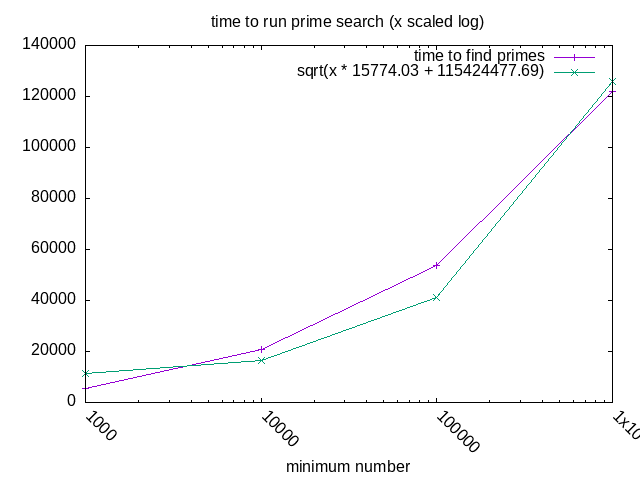
\includegraphics[width=.9\linewidth]{1/fig/1-22-1.png}
\end{center}

The plot for the square root function doesn't quite fit the real one and I'm not
sure where the fault lies. I don't struggle to understand things like ``this
algorithm is slower than this other one,'' but when asked to find or prove the
\(\Theta\) notation I'm pretty clueless;
\end{enumerate}

\subsection{Exercise 1.23}
\label{sec:org9381e53}
\subsubsection{Question}
\label{sec:orgeb709cd}
\begin{quote}
The \texttt{smallest-divisor} procedure shown at the start of this section does lots of
needless testing: After it checks to see if the number is divisible by 2 there
is no point in checking to see if it is divisible by any larger even numbers.
This suggests that the values used for test-divisor should not be 2, 3, 4, 5, 6,
…, but rather 2, 3, 5, 7, 9, …. To implement this change, define a procedure
\texttt{next} that returns 3 if its input is equal to 2 and otherwise returns its input
plus 2. Modify the smallest-divisor procedure to use \mintinline[breaklines=true,breakanywhere=true,linenos=true]{scheme}{(next test-divisor)} instead of \mintinline[breaklines=true,breakanywhere=true,linenos=true]{scheme}{(+ test-divisor 1)}. With
\texttt{timed-prime-test} incorporating this modified version of \texttt{smallest-divisor},
run the test for each of the 12 primes found in Exercise 1.22. Since this
modification halves the number of test steps, you should expect it to run about
twice as fast. Is this expectation confirmed? If not, what is the observed ratio
of the speeds of the two algorithms, and how do you explain the fact that it is
different from 2?
\end{quote}
\subsubsection{A Comedy of Error (just the one)}
\label{sec:orgd0c8f77}
\begin{minted}[breaklines=true,breakanywhere=true,linenos=true]{scheme}
<<square>>
(define (smallest-divisor n)
  (find-divisor n 2))

(define (next n)
  (if (= n 2)
      3
      (+ n 1)))

(define (find-divisor n test-divisor)
  (cond ((> (square test-divisor) n) 
         n)
        ((divides? test-divisor n) 
         test-divisor)
        (else (find-divisor 
               n 
               (next test-divisor)))))

(define (divides? a b)
  (= (remainder b a) 0))
\end{minted}
\begin{minted}[breaklines=true,breakanywhere=true,linenos=true]{scheme}
<<mattbench2>>
<<find-divisor-faster>>
(define (prime? n)
  (= n (smallest-divisor n)))
<<search-for-primes-untimed>>
<<print-table>>

(define benchmark-iterations 1000000)
(define (testit f)
  (list (cadr (mattbench2 (λ() (f 1000 3)) benchmark-iterations))
        (cadr (mattbench2 (λ() (f 10000 3)) benchmark-iterations))
        (cadr (mattbench2 (λ() (f 100000 3)) benchmark-iterations))
        (cadr (mattbench2 (λ() (f 1000000 3)) benchmark-iterations))))

(print-row
 (testit search-for-primes))
\end{minted}

\begin{table}[htbp]
\label{1-22-smdf}
\centering
\begin{tabular}{rrrr}
6456.538118 & 25550.757304 & 66746.041644 & 148505.580638\\
\end{tabular}
\end{table}


\begin{center}
\begin{tabular}{rrr}
min & (+1) & (next)\\
1000 & 5507.42497 & 6366.99462\\
10000 & 20913.71497 & 24845.9193\\
100000 & 53778.74737 & 64756.73693\\
1000000 & 122135.60511 & 143869.63561\\
\end{tabular}
\end{center}

\begin{center}
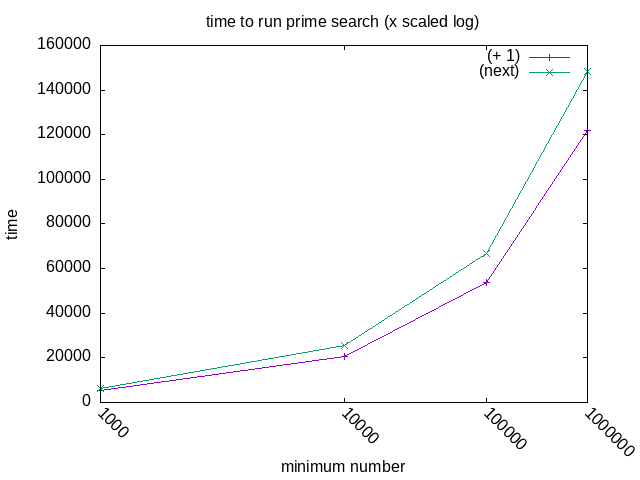
\includegraphics[width=.9\linewidth]{1/fig/1-22-2.png}
\end{center}

So it's \emph{slower} than before. Why?

Oh, that's why.
\begin{minted}[breaklines=true,breakanywhere=true,linenos=true]{scheme}
(define (next n)
  (if (= n 2)
      3
      (+ n 1))) ;; <-- D'oh.
\end{minted}

\subsubsection{Answer}
\label{sec:org4b673e8}
Ok, let's try that again.

\begin{minted}[breaklines=true,breakanywhere=true,linenos=true]{scheme}
<<square>>
(define (smallest-divisor n)
  (find-divisor n 2))

(define (next n)
  (if (= n 2)
      3
      (+ n 2)))

(define (find-divisor n test-divisor)
  (cond ((> (square test-divisor) n) 
         n)
        ((divides? test-divisor n) 
         test-divisor)
        (else (find-divisor 
               n 
               (next test-divisor)))))

(define (divides? a b)
  (= (remainder b a) 0))
\end{minted}
\begin{minted}[breaklines=true,breakanywhere=true,linenos=true]{scheme}
<<mattbench2>>
<<find-divisor-faster-real>>
(define (prime? n)
  (= n (smallest-divisor n)))
<<search-for-primes-untimed>>
<<print-table>>

(define benchmark-iterations 500000)
(define (testit f)
  (list (cadr (mattbench2 (λ() (f 1000 3)) benchmark-iterations))
        (cadr (mattbench2 (λ() (f 10000 3)) benchmark-iterations))
        (cadr (mattbench2 (λ() (f 100000 3)) benchmark-iterations))
        (cadr (mattbench2 (λ() (f 1000000 3)) benchmark-iterations))))

(print-row
 (testit search-for-primes))
\end{minted}

\begin{table}[htbp]
\label{1-22-smdff}
\centering
\begin{tabular}{rrrr}
3863.7424 & 13519.209814 & 33520.676384 & 73005.539932\\
\end{tabular}
\end{table}

\begin{center}
\begin{tabular}{rrrr}
min & (+1) & (next-broken) & (next-fixed)\\
--- & --- & --- & ---\\
1000 & 5425.223086 & 6456.538118 & 3863.7424\\
10000 & 20772.332491 & 25550.757304 & 13519.209814\\
100000 & 53577.240193 & 66746.041644 & 33520.676384\\
1000000 & 121986.712395 & 148505.580638 & 73005.539932\\
\end{tabular}
\end{center}

\begin{center}
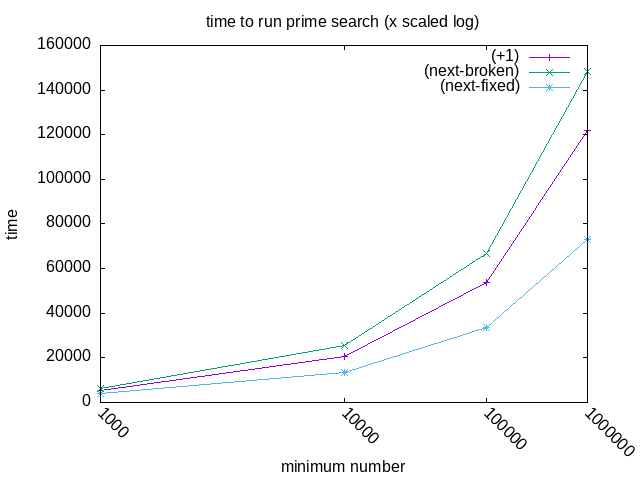
\includegraphics[width=.9\linewidth]{1/fig/1-22-3.png}
\end{center}

I had a lot of trouble getting this one to compile, I have to restart Emacs in
order to get it to render.

Anyways, there's the speedup that was expected. Let's compare the ratios.

Defining a new average that takes arbitrary numbers of arguments:
\begin{minted}[breaklines=true,breakanywhere=true,linenos=true]{scheme}
(define (average . args)
  (let ((len (length args)))
    (/ (apply + args) len)))
\end{minted}

Using it for percentage comparisons:
\begin{minted}[breaklines=true,breakanywhere=true,linenos=true]{scheme}
<<average-varargs>>
(list (cons "% speedup for broken (next)"
            (cons (format #f "~2$%"
                          (apply average
                                 (map (λ (x y) (* 100 (/ x y)))
                                      (car smd) (car smdf))))
                  #nil))
      (cons "% speedup for real (next)"
            (cons (format #f "~2$%"
                          (apply average
                                 (map (λ (x y) (* 100 (/ x y)))
                                      (car smd) (car smdff))))
                  #nil)))
\end{minted}

\begin{center}
\begin{tabular}{ll}
\% speedup for broken (next) & 81.93\%\\
\% speedup for real (next) & 155.25\%\\
\end{tabular}
\end{center}

Since this changed algorithm cuts out almost half of the steps, you might expect
something more like a 200\% speedup. Let's try optimizing it further. Two observations:

\begin{enumerate}
\item The condition \mintinline[breaklines=true,breakanywhere=true,linenos=true]{scheme}{(divides? 2 n)} only needs to be run once at the
start of the program.
\item Because it only needs to be run once, it doesn't need to be a separate
function at all.
\end{enumerate}

\begin{minted}[breaklines=true,breakanywhere=true,linenos=true]{scheme}
<<square>>
(define (smallest-divisor n)
  (if (divides? 2 n)                  ;; check for division by 2
      2
      (find-divisor n 3)))            ;; start find-divisor at 3

(define (find-divisor n test-divisor)
  (cond ((> (square test-divisor) n) 
         n)
        ((divides? test-divisor n) 
         test-divisor)
        (else (find-divisor 
               n 
               (+ 2 test-divisor))))) ;; just increase by 2

(define (divides? a b)
  (= (remainder b a) 0))
\end{minted}
\begin{minted}[breaklines=true,breakanywhere=true,linenos=true]{scheme}
<<mattbench2>>
<<find-divisor-faster-real2>>
(define (prime? n)
  (= n (smallest-divisor n)))
<<search-for-primes-untimed>>
<<print-table>>

(define benchmark-iterations 500000)
(define (testit f)
  (list (cadr (mattbench2 (λ() (f 1000 3)) benchmark-iterations))
        (cadr (mattbench2 (λ() (f 10000 3)) benchmark-iterations))
        (cadr (mattbench2 (λ() (f 100000 3)) benchmark-iterations))
        (cadr (mattbench2 (λ() (f 1000000 3)) benchmark-iterations))))

(print-row
 (testit search-for-primes))
\end{minted}


\begin{table}[htbp]
\label{1-22-smdff2}
\centering
\begin{tabular}{rrrr}
3151.259574 & 11245.20428 & 27803.067944 & 61997.275154\\
\end{tabular}
\end{table}

\begin{center}
\begin{tabular}{rrrrr}
min & (+1) & (next-broken) & (next-fixed) & integrated\\
--- & --- & --- & --- & ---\\
1000 & 5425.223086 & 6456.538118 & 3863.7424 & 3151.259574\\
10000 & 20772.332491 & 25550.757304 & 13519.209814 & 11245.20428\\
100000 & 53577.240193 & 66746.041644 & 33520.676384 & 27803.067944\\
1000000 & 121986.712395 & 148505.580638 & 73005.539932 & 61997.275154\\
\end{tabular}
\end{center}

\begin{center}
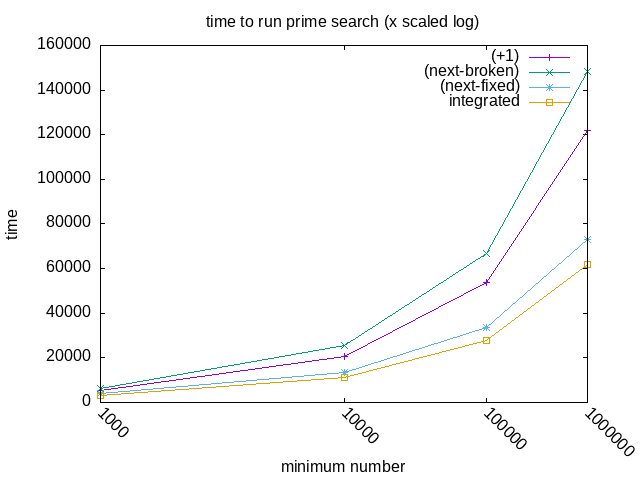
\includegraphics[width=.9\linewidth]{1/fig/1-22-4.png}
\end{center}

\begin{center}
\begin{tabular}{ll}
\% speedup for broken (next) & 81.93\%\\
\% speedup for real (next) & 155.25\%\\
\% speedup for optimized & 186.59\%\\
\end{tabular}
\end{center}

\subsection{Exercise 1.24}
\label{sec:org80fc7ca}
\subsubsection{Text}
\label{sec:org122cb38}
\begin{minted}[breaklines=true,breakanywhere=true,linenos=true]{scheme}
<<square>>
(define (expmod base exp m)
  (cond ((= exp 0) 1)
        ((even? exp)
         (remainder 
          (square (expmod base (/ exp 2) m))
          m))
        (else
         (remainder 
          (* base (expmod base (- exp 1) m))
          m))))
\end{minted}
\begin{minted}[breaklines=true,breakanywhere=true,linenos=true]{scheme}
(define (fermat-test n)
  (define (try-it a)
    (= (expmod a n n) a))
  (try-it (+ 1 (random (- n 1)))))
\end{minted}
\begin{minted}[breaklines=true,breakanywhere=true,linenos=true]{scheme}
(define (fast-prime? n times)
  (cond ((= times 0) #t)
        ((fermat-test n) 
         (fast-prime? n (- times 1)))
        (else #f)))
\end{minted}
\subsubsection{Question}
\label{sec:orge74879a}
\begin{quote}
Modify the \texttt{timed-prime-test} procedure of Exercise 1.22 to use \texttt{fast-prime?} (the
Fermat method), and test each of the 12 primes you found in that exercise. Since
the Fermat test has \(\Theta(\text{log}n)\) growth, how would you expect the
time to test primes near 1,000,000 to compare with the time needed to test
primes near 1000? Do your data bear this out? Can you explain any discrepancy
you find?
\end{quote}

\subsubsection{Answer}
\label{sec:org723bbd8}
\begin{minted}[breaklines=true,breakanywhere=true,linenos=true]{scheme}
<<mattbench2>>
<<expmod>>
<<fermat-test>>
<<fast-prime>>
(define fermat-iterations 2)
(define (prime? n)
  (fast-prime? n fermat-iterations))
<<search-for-primes-untimed>>
<<print-table>>

(define benchmark-iterations 500000)
(define (testit f)
  (list (cadr (mattbench2 (λ() (f 1000 3)) benchmark-iterations))
        (cadr (mattbench2 (λ() (f 10000 3)) benchmark-iterations))
        (cadr (mattbench2 (λ() (f 100000 3)) benchmark-iterations))
        (cadr (mattbench2 (λ() (f 1000000 3)) benchmark-iterations))))

(print-row
 (testit search-for-primes))
\end{minted}

\begin{table}[htbp]
\label{1-24-fermat}
\centering
\begin{tabular}{rrrr}
11175.799722 & 23518.62116 & 32150.745642 & 32679.766448\\
\end{tabular}
\end{table}

\begin{center}
\begin{tabular}{rrrr}
min & (+1) & integrated & fermat (2 guesses)\\
--- & --- & --- & ---\\
1000 & 5425.223086 & 3151.259574 & 11175.799722\\
10000 & 20772.332491 & 11245.20428 & 23518.62116\\
100000 & 53577.240193 & 27803.067944 & 32150.745642\\
1000000 & 121986.712395 & 61997.275154 & 32679.766448\\
\end{tabular}
\end{center}

\begin{center}
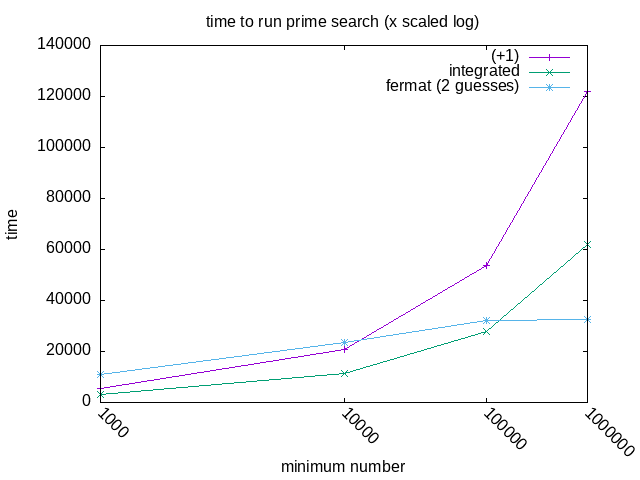
\includegraphics[width=.9\linewidth]{1/fig/1-24-1.png}
\end{center}

It definitely looks to be advancing much slower than the other methods. I'd like
to see more of the function.

\begin{minted}[breaklines=true,breakanywhere=true,linenos=true]{scheme}
<<mattbench2>>
<<find-divisor-faster-real>>
(define (prime? n)
  (= n (smallest-divisor n)))
<<search-for-primes-untimed>>
<<print-table>>

(define benchmark-iterations 100000)
(define (testit f)
  (list (cadr (mattbench2 (λ() (f 1000 3)) benchmark-iterations))
        (cadr (mattbench2 (λ() (f 10000 3)) benchmark-iterations))
        (cadr (mattbench2 (λ() (f 100000 3)) benchmark-iterations))
        (cadr (mattbench2 (λ() (f 1000000 3)) benchmark-iterations))
        (cadr (mattbench2 (λ() (f 10000000 3)) benchmark-iterations))
        (cadr (mattbench2 (λ() (f 100000000 3)) benchmark-iterations))
        (cadr (mattbench2 (λ() (f 1000000000 3)) benchmark-iterations))
        (cadr (mattbench2 (λ() (f 10000000000 3)) benchmark-iterations))
        (cadr (mattbench2 (λ() (f 100000000000 3)) benchmark-iterations))
        (cadr (mattbench2 (λ() (f 1000000000000 3)) benchmark-iterations))))

(print-row
 (testit search-for-primes))
\end{minted}

\begin{minted}[breaklines=true,breakanywhere=true,linenos=true]{scheme}
<<mattbench2>>
<<expmod>>
<<fermat-test>>
<<fast-prime>>
(define fermat-iterations 100)
(define (prime? n)
  (fast-prime? n fermat-iterations))
<<search-for-primes-untimed>>
<<print-table>>

(define benchmark-iterations 100000)
(define (testit f)
  (list (cadr (mattbench2 (λ() (f 1000 3)) benchmark-iterations))
        (cadr (mattbench2 (λ() (f 10000 3)) benchmark-iterations))
        (cadr (mattbench2 (λ() (f 100000 3)) benchmark-iterations))
        (cadr (mattbench2 (λ() (f 1000000 3)) benchmark-iterations))
        (cadr (mattbench2 (λ() (f 10000000 3)) benchmark-iterations))
        (cadr (mattbench2 (λ() (f 100000000 3)) benchmark-iterations))
        (cadr (mattbench2 (λ() (f 1000000000 3)) benchmark-iterations))
        (cadr (mattbench2 (λ() (f 10000000000 3)) benchmark-iterations))
        (cadr (mattbench2 (λ() (f 100000000000 3)) benchmark-iterations))
        (cadr (mattbench2 (λ() (f 1000000000000 3)) benchmark-iterations))))

(print-row
 (testit search-for-primes))
\end{minted}

\begin{center}
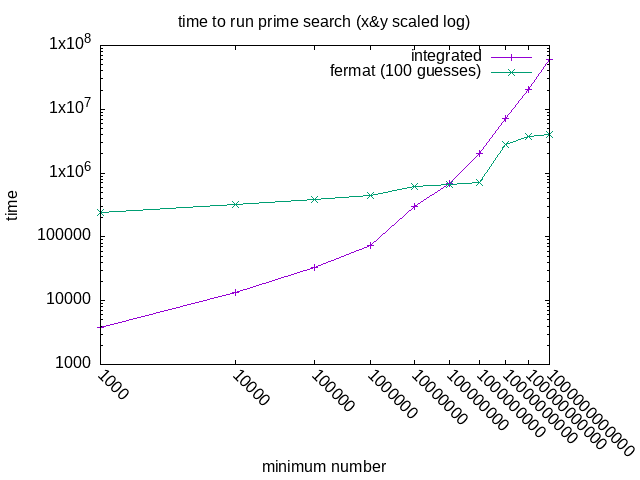
\includegraphics[width=.9\linewidth]{1/fig/1-24-2.png}
\end{center}

For the life of me I have no idea what that bump is. Maybe it needs more
aggressive bignum processing there?

\subsection{Exercise 1.25}
\label{sec:orgb69b00e}
\subsubsection{Question}
\label{sec:org6f8a2bf}
\begin{quote}
Alyssa P. Hacker complains that we went to a lot of extra work in writing
\texttt{expmod}. After all, she says, since we already know how to compute
exponentials, we could have simply written
\end{quote}

\begin{minted}[breaklines=true,breakanywhere=true,linenos=true]{scheme}
(define (expmod base exp m)
  (remainder (fast-expt base exp) m))
\end{minted}

\begin{quote}
Is she correct? Would this procedure serve as well for our fast prime tester?
Explain.
\end{quote}

\subsubsection{Answer}
\label{sec:orge196df1}
In Alyssa's version of \texttt{expmod}, the result of the \texttt{fast-expt} operation is
\emph{extremely} large. For example, in the process of checking for divisors of
1,001, the number 455 will be tried. \mintinline[breaklines=true,breakanywhere=true,linenos=true]{scheme}{(expt 455 1001)} produces an
integer 2,661 digits long. This is just one of the thousands of exponentiations
that \texttt{smallest-divisor} will perform. It's best to avoid this, so we use to our
advantage the fact that we only need to know the remainder of the
exponentiations. \texttt{expmod} breaks down the exponentiation into smaller steps and
performs \texttt{remainder} after every step, significantly reducing the memory
requirements.

As an example, let's trace (some of) the execution of \mintinline[breaklines=true,breakanywhere=true,linenos=true]{scheme}{(expmod 455 1001 1001)}:

\begin{minted}[breaklines=true,breakanywhere=true,linenos=true]{scheme}
(expmod 455 1001 1001)
>  (even? 1001)
>  #f
>  (expmod 455 1000 1001)
>  >  (even? 1000)
>  >  #t
>  >  (expmod 455 500 1001)
>  >  >  (even? 500)
>  >  >  #t
;; ...
>  >  >  x11 (expmod 455 2 1001)
>  >  >  x11 >  (even? 2)
>  >  >  x11 >  #t
>  >  >  x11 >  (expmod 455 1 1001)
>  >  >  x11 >  >  (even? 1)
>  >  >  x11 >  >  #f
>  >  >  x11 >  >  (expmod 455 0 1001)
>  >  >  x11 >  >  1
>  >  >  x11 >  455
>  >  >  x11 >  (square 455)
>  >  >  x11 >  207025
>  >  >  x11 819
;; ...
>  >  >  (square 364)
>  >  >  132496
>  >  364
>  >  (square 364)
>  >  132496
>  364
455
\end{minted}

You can see that the numbers remain quite manageable throughout this process. So
taking these extra steps actually leads to an algorithm that performs better.

\subsection{Exercise 1.26}
\label{sec:org0aad372}
\subsubsection{Question}
\label{sec:orgc9ebaab}
\begin{quote}
Louis Reasoner is having great difficulty doing Exercise 1.24. His \texttt{fast-prime?}
test seems to run more slowly than his \texttt{prime?} test. Louis calls his friend Eva
Lu Ator over to help. When they examine Louis’s code, they find that he has
rewritten the \texttt{expmod} procedure to use an explicit multiplication, rather than
calling \texttt{square}:
\end{quote}

\begin{minted}[breaklines=true,breakanywhere=true,linenos=true]{scheme}
(define (expmod base exp m)
  (cond ((= exp 0) 1)
        ((even? exp)
         (remainder 
          (* (expmod base (/ exp 2) m) ;; <== hmm.
             (expmod base (/ exp 2) m))
          m))
        (else
         (remainder 
          (* base 
             (expmod base (- exp 1) m))
          m))))
\end{minted}

\begin{quote}
“I don’t see what difference that could make,” says Louis. “I do.” says Eva. “By
writing the procedure like that, you have transformed the \(\Theta(\log n)\)
process into a \(\Theta(n)\) process.” Explain.
\end{quote}

\subsubsection{Answer}
\label{sec:org517ee64}
Making the same function call twice isn't the same as using a variable twice --
Louis' version doubles the work, having two processes solving the exact same
problem. Since the number of processes used increases exponentially, this turns
\(\log n\) into \(n\).

\subsection{Exercise 1.27}
\label{sec:org469ccf1}
\subsubsection{Question}
\label{sec:org21eb7e6}
\begin{quote}
Demonstrate that the Carmichael numbers listed in Footnote 1.47 really do fool
the Fermat test. That is, write a procedure that takes an integer \(n\) and
tests whether \(a^n\) is congruent to \(a\) modulo \(n\) for every \(a < n\),
and try your procedure on the given Carmichael numbers.
\end{quote}
\begin{table}[htbp]
\label{carmichael}
\centering
\begin{tabular}{rrrrrr}
561 & 1105 & 1729 & 2465 & 2821 & 6601\\
\end{tabular}
\end{table}
\subsubsection{Answer}
\label{sec:org86e3285}
\begin{minted}[breaklines=true,breakanywhere=true,linenos=true]{scheme}
<<expmod>>
(define (car-test n)
  (define (check a)
    (= (remainder (expt a n) n)
       (remainder (modulo a n) n)))
  (every check
           (cddr (iota n))))
\end{minted}

\begin{minted}[breaklines=true,breakanywhere=true,linenos=true]{scheme}
<<car-test>>
(list (car-test 12) ; <== false (not prime)
      (car-test 1009);<== true  (real prime)
      (car-test 561));<== true  (not prime,
                     ;      Carmichael number)
\end{minted}

\subsection{Exercise 1.28}
\label{sec:org1c66fc6}
\subsubsection{Question}
\label{sec:org6c3ed71}
\begin{quote}
One variant of the Fermat test that cannot be fooled is called the Miller-Rabin
test (Miller 1976; Rabin 1980). This starts from an alternate form of Fermat’s
Little Theorem, which states that if \(n\) is a prime number and \(a\) is
any positive integer less than \(n\), then \(a\) raised to the \((n−1)\)
-st power is congruent to 1 modulo \(n\). To test the primality of a number \(n\) by the Miller-Rabin test, we pick a random number \(a<n\) and raise \(a\) to the \((n−1)\) -st power modulo \(n\) using the \texttt{expmod} procedure.
However, whenever we perform the squaring step in \texttt{expmod}, we check to see if
we have discovered a “nontrivial square root of 1 modulo \(n\),” that is, a
number not equal to 1 or \(n−1\) whose square is equal to 1 modulo \(n\). It
is possible to prove that if such a nontrivial square root of 1 exists, then \(n\) is not prime. It is also possible to prove that if \(n\) is an odd number
that is not prime, then, for at least half the numbers \(a<n\), computing \(an−1\) in this way will reveal a nontrivial square root of 1 modulo \(n\).
(This is why the Miller-Rabin test cannot be fooled.) Modify the \texttt{expmod}
procedure to signal if it discovers a nontrivial square root of 1, and use this
to implement the Miller-Rabin test with a procedure analogous to fermat-test.
Check your procedure by testing various known primes and non-primes. Hint: One
convenient way to make \texttt{expmod} signal is to have it return 0.
\end{quote}
\subsubsection{Analysis}
\label{sec:org0de1865}
For the sake of verifying this, I want to get a bigger list of primes and
Carmichael numbers to verify against. I'll save them using Guile's built in
read/write functions that save Lisp lists to text:
\begin{minted}[breaklines=true,breakanywhere=true,linenos=true]{scheme}
<<find-divisor-faster-real>>
(define (prime? n)
  (= n (smallest-divisor n)))
(call-with-output-file "Data/primes-1k_to_1mil.txt" (λ(port)
  (write (filter prime? (iota (- 1000000 1000) 1000))
         port)))
\end{minted}

\begin{minted}[breaklines=true,breakanywhere=true,linenos=true]{scheme}
;; fermat prime test but checks *every* value from 2 to n-1
(define (fermat-prime? n)
  (define (iter a)
    (if (= a n)
        #f
        (if (= (expmod a n n) a)
            #t
            (iter (+ 1 a)))))
  (iter 2))
\end{minted}

\begin{minted}[breaklines=true,breakanywhere=true,linenos=true]{scheme}
(use-srfis '(1))
<<expmod>>
<<fermat-prime?>>
<<find-divisor-faster-real>>
(define (prime? n)
  (= n (smallest-divisor n)))
(call-with-output-file "Data/carmichael-verification.txt" (λ(port)
     (write (filter
             (λ(x) (and (fermat-prime? x)
                        (not (prime? x))))
             (iota (- 1000000 1000) 1000))
            port)))
\end{minted}

This will be useful in various future functions:
\begin{minted}[breaklines=true,breakanywhere=true,linenos=true]{scheme}
(define list-of-primes (call-with-input-file "Data/primes-1k_to_1mil.txt" read))
(define list-of-carmichaels (call-with-input-file "Data/carmichael.txt" read))
\end{minted}

\begin{minted}[breaklines=true,breakanywhere=true,linenos=true]{scheme}
(use-srfis '(1))
<<expmod>>
<<fermat-prime?>>
<<find-divisor-faster-real>>
(define (prime? n)
  (= n (smallest-divisor n)))
<<get-lists-of-primes>>
(define prime-is-working
  (and (and-map prime? list-of-primes)
       (not (and-map prime? list-of-carmichaels))))
(format #t "(prime?) is working: ~a~%"
        (if prime-is-working
            "Yes"
            "No"))
(define fermat-is-vulnerable
  (and (and-map fermat-prime? list-of-primes)
       (and-map fermat-prime? list-of-carmichaels)))
(format #t "(fermat-prime?) is vulnerable: ~a~%"
        (if fermat-is-vulnerable
            "Yes"
            "No"))
\end{minted}

\begin{verbatim}
(prime?) is working: Yes
(fermat-prime?) is vulnerable: Yes
\end{verbatim}

\subsubsection{Answer}
\label{sec:orgbe9edcb}
\begin{minted}[breaklines=true,breakanywhere=true,linenos=true]{scheme}
<<square>>
(define (expmod-mr base exp m)
  (cond ((= exp 0) 1)
        ((even? exp)
         (let ((sqr
                (square (expmod-mr base (/ exp 2) m))))
           (if (= 1 (modulo sqr m))
               0
               (remainder sqr m))))
        (else
         (remainder 
          (* base (expmod-mr base (- exp 1) m))
          m))))
\end{minted}
\begin{minted}[breaklines=true,breakanywhere=true,linenos=true]{scheme}
(define (mr-test n)
  (define (try-it a)
    (let ((it (expmod-mr a n n)))
      (or (= it a)
          (= it 0))))
  (try-it (+ 1 (random (- n 1)))))
\end{minted}
\begin{minted}[breaklines=true,breakanywhere=true,linenos=true]{scheme}
(define (mr-prime? n times)
  (cond ((= times 0) #t)
        ((mr-test n) 
         (mr-prime? n (- times 1)))
        (else #f)))
\end{minted}

\begin{minted}[breaklines=true,breakanywhere=true,linenos=true]{scheme}
<<expmod-mr>>
<<mr-test>>
<<mr-prime>>
(define mr-times 100)
<<get-lists-of-primes>>
(format #t "      mr detects primes: ~a~%mr false-positives Carmichaels: ~a~%"
        (and-map (λ(x)(mr-prime? x mr-times)) list-of-primes)
      (and-map (λ(x)(mr-prime? x mr-times)) list-of-carmichaels))
\end{minted}

\begin{verbatim}
      mr detects primes: #t
mr false-positives Carmichaels: #t
\end{verbatim}

Shoot. And I thought I did a very literal interpretation of what the book asked.

Ah, I see the problem. I need to keep track of what the pre-squaring number was
and use that to determine whether the square is valid or not.

\begin{minted}[breaklines=true,breakanywhere=true,linenos=true]{scheme}
<<square>>
(define (expmod-mr base exp m)
  (cond ((= exp 0) 1)
        ((even? exp)
         ;; Keep result and remainder seperate
         (let* ((result (expmod-mr base (/ exp 2) m))
                (rem (remainder (square result) m)))
           (if (and (not (= result 1))
                    (not (= result (- m 1)))
                    (= 1 rem))
               0 ;; non-trivial sqrt mod 1 is found
               rem)))
        (else
         (remainder 
          (* base (expmod-mr base (- exp 1) m))
          m))))
\end{minted}
Unfortunately this one has the same problem. What's the issue?

Sadly, there's a massive issue in \texttt{mr-test}.
\begin{minted}[breaklines=true,breakanywhere=true,linenos=true]{scheme}
(define (mr-test n)
  (define (try-it a)
    (let ((it (expmod-mr a n n))) ;; Should be "a (- n 1) n"
      (or (= it a)    ;; Should be (= it 1)
          (= it 0)))) ;; Two strikes, you're out
  (try-it (+ 1 (random (- n 1)))))
\end{minted}

One more time.
\begin{minted}[breaklines=true,breakanywhere=true,linenos=true]{scheme}
(define (mr-test n)
  (define (try-it a)
    (= 1 (expmod-mr a (- n 1) n)))
  (try-it (+ 1 (random (- n 1)))))
\end{minted}

\begin{minted}[breaklines=true,breakanywhere=true,linenos=true]{scheme}
<<expmod-mr2>>
<<mr-test2>>
<<mr-prime>>
(define mr-times 100)
<<get-lists-of-primes>>
(format #t "      mr detects primes: ~a~%mr false-positives Carmichaels: ~a~%"
        (and-map (λ(x)(mr-prime? x mr-times)) list-of-primes)
      (and-map (λ(x)(mr-prime? x mr-times)) list-of-carmichaels))
\end{minted}

\begin{verbatim}
     mr detects primes: #t
mr false-positives Carmichaels: #f
\end{verbatim}

\subsection{1.3: Formulating Abstractions with Higher-Order Procedures}
\label{sec:org9d0bf8f}
Procedures that manipulate procedures are called \emph{higher-order procedures}.
\subsection{1.3.1: Procedures as Arguments}
\label{sec:org2a49263}
Let's say we have several different types of series that we want to sum.
Functions for each of these tasks will look very similar, so we're better off
defining a general function that expresses the \emph{idea} of summation, that can
then be passed specific functions to cause the specific behavior of the series.
Mathematicians express this as \(\sum\) (``sigma'') notation.

For the program:

\begin{minted}[breaklines=true,breakanywhere=true,linenos=true]{scheme}
(define (sum term a next b)
  (if (> a b)
      0
      (+ (term a)
         (sum term (next a) next b))))
\end{minted}

Which is equivalent to:

\[\sum^{b}_{n~a}term(n)~term(a)+term(next(a))+term(next(next(a)))+\cdots+term(b)\]

We can pass integers to \texttt{a} and \texttt{b} and functions to \texttt{term} and \texttt{next}. Note
that in order to simply sum integers, we'd need to define and pass an identity
function to \texttt{term}.
\subsection{Exercise 1.29}
\label{sec:org9eb91af}
\subsubsection{Text}
\label{sec:org9a19bcb}
\begin{minted}[breaklines=true,breakanywhere=true,linenos=true]{scheme}
(define (sum term a next b)
  (if (> a b)
      0
      (+ (term a)
         (sum term (next a) next b))))
\end{minted}
\begin{minted}[breaklines=true,breakanywhere=true,linenos=true]{scheme}
(define (integral f a b dx)
  (define (add-dx x)
    (+ x dx))
  (* (sum f (+ a (/ dx 2.0)) add-dx b)
     dx))
\end{minted}
\subsubsection{Question}
\label{sec:orgfe0729a}
\begin{quote}
Simpson's Rule is a more accurate method of numerical integration than the
method illustrated above. Using Simpson's Rule, the integral of a function \(f\)
between \(a\) and \(b\) is approximated as

\[
{h\over 3}(y_0 + 4y_1 + 2y_2 + 4y_3 + 2y_4 + \dots + 2y_{n-2} + 4y_{n-1} + y_n)
\]

where \(h = (b - a) / n\), for some even integer \(n\), and \(y_k = f(a + kh)\).
(Increasing \(n\) increases the accuracy of the approximation.) Define a
procedure that takes as arguments \(f\), \(a\), \(b\), and \(n\) and returns the
value of the integral, computed using Simpson's Rule. Use your procedure to
integrate \texttt{cube} between 0 and 1 (with \(n = 100\) and \(n = 1000\)), and
compare the results to those of the \texttt{integral} procedure shown above.
\end{quote}
\subsubsection{Answer}
\label{sec:orgc21f714}
\begin{minted}[breaklines=true,breakanywhere=true,linenos=true]{scheme}
(define (int-simp f a b n)
  (define h
    (/ (- b a)
     n))
  (define (gety k)
    (f (+ a (* k h))))
  (define (series-y sum k) ;; start with sum = y_0
    (cond ((= k n) (+ sum (gety k)));; and k = 1
          ((even? k) (series-y
                      (+ sum (* 2 (gety k)))
                      (+ 1 k)))
          (else (series-y
                 (+ sum (* 4 (gety k)))
                 (+ 1 k)))))
  (define sum-of-series (series-y (gety a) 1)) ;; (f a) = y_0
  (* (/ h 3) sum-of-series))
\end{minted}

Let's compare these at equal levels of computational difficulty.
\begin{minted}[breaklines=true,breakanywhere=true,linenos=true]{scheme}
<<mattbench2>>
<<print-table>>
(define (cube x)
  (* x x x))
<<sum>>
<<integral>>
<<int-simp>>

(define iterations 100000) ;; benchmark iterations
(define (run-test1)
  (integral cube 0.0 1.0 0.0008))
(define (run-test2)
  (int-simp cube 0.0 1.0 1000.0))
(print-table (list (list "integral dx:0.0008" "int-simp i:1000")
                   (list (run-test1) (run-test2))
                   (list (cadr (mattbench2 run-test1 iterations))
                         (cadr (mattbench2 run-test2 iterations))))
             #:colnames #t)
\end{minted}

\begin{center}
\begin{tabular}{rr}
integral dx:0.0008 & int-simp i:1000\\
\hline
0.24999992000001311 & 0.25000000000000006\\
321816.2755 & 330405.8918\\
\end{tabular}
\end{center}

So, more accurate for roughly the same effort or less.

\subsection{Exercise 1.30}
\label{sec:orgfa06cc4}
\subsubsection{Question}
\label{sec:org79164d8}
\begin{quote}
The \texttt{sum} procedure above generates a linear recursion. The procedure can be
rewritten so that the sum is performed iteratively. Show how to do this by
filling in the missing expressions in the following definition:
\end{quote}

\subsubsection{Answer}
\label{sec:org86ee004}
\begin{minted}[breaklines=true,breakanywhere=true,linenos=true]{scheme}
(define (sum-iter term a next b)
  (define (iter a result)
    (if (> a b)
        result
        (iter (next a) (+ result (term a)))))
  (iter a 0))
\end{minted}

Let's check the stats!
\begin{center}
\begin{tabular}{rr}
recursive & iterative\\
\hline
30051.080005 & 19568.685587\\
\end{tabular}
\end{center}

\subsection{Exercise 1.31}
\label{sec:org7ad1039}
\subsubsection{Question A.1}
\label{sec:org7cec7d7}
\begin{quote}
The \texttt{sum} procedure is only the simplest of a vast number of similar
abstractions that can be captured as higher-order procedures. Write an analogous
procedure called \texttt{product} that returns the product of the values of a function
at points over a given range.
\end{quote}
\subsubsection{Answer A.1}
\label{sec:org11a2e65}
\begin{minted}[breaklines=true,breakanywhere=true,linenos=true]{scheme}
(define (product-iter term a next b)
  (define (iter a result)
    (if (> a b)
        result
        (iter (next a) (* result (term a)))))
  (iter a 1)) ;; start at 1 so it's not always 0
\end{minted}
\subsubsection{Question A.2}
\label{sec:org1a59ec1}
\begin{quote}
Show how to define \texttt{factorial} in terms of \texttt{product}.
\end{quote}
\subsubsection{Answer A.2}
\label{sec:org5121a9e}
I was briefly stumped because \texttt{product} only counts upward. Then I realized
that's just how it's presented and it can go either direction, since addition
and multiplication are commutative. I look forward to building up a more
intuitive sense of numbers.
\begin{minted}[breaklines=true,breakanywhere=true,linenos=true]{scheme}
<<product-iter>>
(define (identity x)
  x)
(define (inc x)
  (1+ x))

(define (factorial n)
  (product-iter identity 1 inc n))

(display (factorial 7))
\end{minted}

\subsubsection{Question A.3}
\label{sec:orge4e7141}
\begin{quote}
Also use \texttt{product} to compute approximations to \(\pi\) using the formula

\[
{\pi\over 4} = {2\cdot 4\cdot 4\cdot 6\cdot 6\cdot 8\cdots\over
		   3\cdot 3\cdot 5\cdot 5\cdot 7\cdot 7\cdots}
\]
\end{quote}

\subsubsection{Answer A.3}
\label{sec:org5c59f55}
Once this equation is encoded, you just need to multiply it by two to get \(\pi\).

Fun fact: the formula is slightly wrong, it should start the series with \({1 \over 2}\).
\begin{minted}[breaklines=true,breakanywhere=true,linenos=true]{scheme}
<<product-iter>>
(define (pi-product n)
  (define (div x)
    (let ((x1 (- x 1))
          (x2 (+ x 1)))
      (* (/ x x1) (/ x x2))))
  (* 2.0 (product-iter div 2 (lambda (z) (+ z 2)) n)))

(display (pi-product 100000))
\end{minted}

\begin{verbatim}
3.1415769458228726
\end{verbatim}

\subsubsection{Question B}
\label{sec:org0845973}
\begin{quote}
If your product procedure generates a recursive process, write one that
generates an iterative process. If it generates an iterative process, write one
that generates a recursive process.
\end{quote}

\subsubsection{Answer B}
\label{sec:orgd7df6cb}
\begin{minted}[breaklines=true,breakanywhere=true,linenos=true]{scheme}
(define (product-rec term a next b)
  (if (> a b)
      1
      (* (term a)
         (product-rec term (next a) next b))))
\end{minted}

\begin{minted}[breaklines=true,breakanywhere=true,linenos=true]{scheme}
<<mattbench2>>
<<print-table>>
<<product-iter>>
(define (pi-product n)
  (define (div x)
    (let ((x1 (- x 1))
          (x2 (+ x 1)))
      (* (/ x x1) (/ x x2))))
  (* 2.0 (product-iter div 2 (lambda (z) (+ z 2)) n)))
<<product-rec>>
(define (pi-product-rec n)
  (define (div x)
    (let ((x1 (- x 1))
          (x2 (+ x 1)))
      (* (/ x x1) (/ x x2))))
  (* 2.0 (product-rec div 2 (lambda (z) (+ z 2)) n)))

(define iterations 50000)
(print-table
 (list (list "iterative" "recursive")
       (list (cadr (mattbench2 (λ()(pi-product 1000)) iterations))
             (cadr (mattbench2 (λ()(pi-product-rec 1000)) iterations))))
 #:colnames #t)
\end{minted}

\begin{center}
\begin{tabular}{rr}
iterative & recursive\\
\hline
1267118.0538 & 3067085.5323\\
\end{tabular}
\end{center}

\subsection{Exercise 1.32}
\label{sec:orge9bdfa6}
\subsubsection{Question A}
\label{sec:org73d9336}
\begin{quote}
Show that \texttt{sum} and \texttt{product} are both special cases of a still more general
notion called \texttt{accumulate} that combines a collection of terms, using some
general accumulation function:
\end{quote}

\begin{minted}[breaklines=true,breakanywhere=true,linenos=true]{scheme}
(accumulate combiner null-value term a next b)
\end{minted}

\begin{quote}
\texttt{accumulate} takes as arguments the same term and range specifications as \texttt{sum}
and \texttt{product}, together with a \texttt{combiner} procedure (of two arguments) that
specifies how the current term is to be combined with the accumulation of the
preceding terms and a \texttt{null-value} that specifies what base value to use when
the terms run out. Write \texttt{accumulate} and show how \texttt{sum} and \texttt{product} can both
be defined as simple calls to \texttt{accumulate}.
\end{quote}

\subsubsection{Answer A}
\label{sec:orgd590bbb}
When I first did this question, I struggled a lot before realizing \texttt{accumulate}
was much closer to the exact definitions of sum/product than I thought.
\begin{minted}[breaklines=true,breakanywhere=true,linenos=true]{scheme}
(define (accumulate-iter combiner null-value term a next b)
  (define (iter a result)
    (if (> a b)
        result
        (iter (next a)
              (combiner result (term a)))))
  (iter a null-value))
\end{minted}

\begin{minted}[breaklines=true,breakanywhere=true,linenos=true]{scheme}
<<accumulate-iter>>

;; here you can see definitions in terms of accumulate
(define (sum term a next b)
  (accumulate-iter + 0 term a next b))
(define (product term a next b)
  (accumulate-iter * 1 term a next b))

(define (identity x)
  x)
(define (inc x)
  (1+ x))

;; accumulate in action
(define (factorial n)
  (accumulate-iter * 1 identity 1 inc n))

(display (factorial 7))
\end{minted}

\begin{verbatim}
5040
\end{verbatim}

\subsubsection{Question B}
\label{sec:orgb156f98}
\begin{quote}
If your \texttt{accumulate} procedure generates a recursive process, write one
that generates an iterative process.  If it generates an iterative process,
write one that generates a recursive process.
\end{quote}

\subsubsection{Answer B}
\label{sec:orgf609e4b}
\begin{minted}[breaklines=true,breakanywhere=true,linenos=true]{scheme}
(define (accumulate-rec combiner null-value term a next b)
  (if (> a b)
      null-value
      (combiner (term a)
         (accumulate-rec combiner null-value
                         term (next a) next b))))
\end{minted}

\subsection{Exercise 1.33}
\label{sec:org3f3573e}
\subsubsection{Question A}
\label{sec:org5c17a80}
\index{filter}
\begin{quote}
You can obtain an even more general version of \texttt{accumulate} by introducing the
notion of a filter on the terms to be combined. That is, combine only those
terms derived from values in the range that satisfy a specified condition. The
resulting \texttt{filtered-accumulate} abstraction takes the same arguments as
accumulate, together with an additional predicate of one argument that specifies
the filter. Write \texttt{filtered-accumulate} as a procedure. 
\end{quote}

\subsubsection{Answer A}
\label{sec:orgd072235}
\begin{minted}[breaklines=true,breakanywhere=true,linenos=true]{scheme}
(define (filtered-accumulate-iter
           predicate? combiner null-value
           term a next b)
  (define (iter a result)
    (cond ((> a b) result)
          ((predicate? a)
           (iter (next a)
                 (combiner result (term a))))
          (else (iter (next a)
                      result))))
  (iter a null-value))
\end{minted}

\subsubsection{Question B}
\label{sec:org97f6f30}
Show how to express the following using \texttt{filtered-accumulate}:

\begin{enumerate}
\item A
\label{sec:org6ef2aa7}
Find the sum of the squares of the prime numbers in the interval \(a\) to \(b\)
(assuming that you have a \texttt{prime?} predicate already written)

\begin{minted}[breaklines=true,breakanywhere=true,linenos=true]{scheme}
(load "mattcheck.scm")
(define (square x)
  (* x x))
<<filtered-accumulate-iter>>
<<expmod-mr2>>
<<mr-test2>>
<<mr-prime>>
(define mr-times 100)
(define (prime? x)
  (mr-prime? x mr-times))
(define (prime-sum a b)
  (filtered-accumulate-iter prime? + 0
                            square a 1+ b))

(mattcheck-equal "1 prime correct"
                 (prime-sum 1008 1010)
                 (square 1009)) ;; 1009
(mattcheck-equal "many primes correct"
                 (prime-sum 1000 2001)
                 (apply +
                        (map square
                             (filter prime? (iota (- 2001 1000)
                                                  1000)))))
\end{minted}

\begin{verbatim}
SUCCEED at 1 prime correct
SUCCEED at many primes correct
\end{verbatim}

\item B
\label{sec:orgd581baf}
\begin{quote}
Find the product of all the positive integers less than \(n\) that are
relatively prime to \(n\) (i.e., all positive integers \(i < n\) such that
\(\textsc{gcd}(i, n) = 1\).
\end{quote}

\begin{minted}[breaklines=true,breakanywhere=true,linenos=true]{scheme}
(load "mattcheck.scm")
(define (square x)
  (* x x))
(define (id x) x)
<<filtered-accumulate-iter>>
<<gcd>>
(define (relative-prime? x y)
  (= 1 (gcd x y)))

(define (Ex_1-33B n)
  (filtered-accumulate-iter
   (λ(i) (relative-prime? i n))
   * 1 id
   1 1+ (1- n)))

(define (alternate n)
  (apply *
         (filter (λ(i) (relative-prime? i n))
                 (iota (- n 1) 1))))

(mattcheck-equal "Ex_1-33B"
                 (Ex_1-33B 100)
                 (alternate 100))
\end{minted}

\begin{verbatim}
SUCCEED at Ex_1-33B
\end{verbatim}
\end{enumerate}

\subsection{1.3.2: Constructing Procedures Using lambda}
\label{sec:org262bf6e}
A procedure that's only used once is more conveniently expressed as the special
form \texttt{lambda}.

Variables that are only briefly used in a limited scope can be specified with
the special form \texttt{let}. Variables in \texttt{let} blocks override external variables.
The authors recommend using \texttt{define} for procedures and \texttt{let} for variables.
\subsection{Exercise 1.34}
\label{sec:org8d5cc82}
\subsubsection{Question}
\label{sec:org507f8e2}
\begin{quote}
Suppose we define the procedure
\end{quote}

\begin{minted}[breaklines=true,breakanywhere=true,linenos=true]{scheme}
(define (f g) (g 2))
\end{minted}

\begin{quote}
Then, we have
\end{quote}

\begin{minted}[breaklines=true,breakanywhere=true,linenos=true]{scheme}
(f square)
; 4
(f (lambda (z) (* z (+ z 1))))
; 6
\end{minted}

\begin{quote}
What happens if we (perversely) ask the interpreter to evaluate the combination
\mintinline[breaklines=true,breakanywhere=true,linenos=true]{scheme}{(f f)}? Explain.
\end{quote}
\subsubsection{Answer}
\label{sec:org574de05}
It ends up trying to execute \texttt{2} as a function.
\begin{minted}[breaklines=true,breakanywhere=true,linenos=true]{scheme}
;; Will be evaluated like this:
;;   (f f)
;;   (f 2)
;;   (2 2)
(define (f g) (g 2))
(f f)
\end{minted}

\begin{verbatim}
ice-9/boot-9.scm:1685:16: In procedure raise-exception:
Wrong type to apply: 2
\end{verbatim}
\subsection{1.3.3 Procedures as General Methods}
\label{sec:org5081a61}
The \textbf{half-interval method}: if \(f(a)<0<f(b)\), then \(f\) must have at least
one 0 between \(a\) and \(b\). To find 0, let \(x\) be the average of \(a\) and
\(b\), if \(f(x) < 0\) then 0 must be between \(x\) and \(b\), if \(f(x)>0\)
than 0 must be between \(a\) and \(x\).

The \textbf{fixed point} of a function satisfies the equation \[f(x)=x\]

For some functions, we can locate a fixed point by beginning with an initial
guess \(y\) and applying \(f(y)\) repeatedly until the value doesn't change
much.

\textbf{Average damping} can help converge fixed-point searches.

The symbol \(\mapsto\) (``maps to'') can be considered equivalent to a lambda. For
example, \(x \mapsto x+x\) is equivalent to \mintinline[breaklines=true,breakanywhere=true,linenos=true]{scheme}{(lambda (x) (+ x x))}. In
English, ``the function whose value at \(y\) is \(x/y\)''. \emph{Though it seems like
\(\mapsto\) doesn't necessarily describe a function, but the value of a function
at a certain point? Or maybe that would just be \(~\), ie \(f(x)~etc\)}
\subsection{Exercise 1.35}
\label{sec:orgea8028d}
\subsubsection{Text}
\label{sec:orgcd1b049}
\begin{minted}[breaklines=true,breakanywhere=true,linenos=true]{scheme}
(define (close-enough? x y) 
  (< (abs (- x y)) 0.001))
\end{minted}

\begin{minted}[breaklines=true,breakanywhere=true,linenos=true]{scheme}
(define tolerance 0.00001)

(define (fixed-point f first-guess)
  (define (close-enough? v1 v2)
    (< (abs (- v1 v2)) 
       tolerance))
  (define (try guess)
    (let ((next (f guess)))
      (if (close-enough? guess next)
          next
          (try next))))
  (try first-guess))
\end{minted}
\subsubsection{Question}
\label{sec:orgd185e27}
\begin{quote}
Show that the golden ratio \(\varphi\) is a fixed point of the transformation
\(x \mapsto 1 + 1 / x\), and use this fact to compute \(\varphi\) by means of
the \texttt{fixed-point} procedure.
\end{quote}
\subsubsection{Answer}
\label{sec:org8322e49}
\begin{minted}[breaklines=true,breakanywhere=true,linenos=true]{scheme}
<<close-enough>>
<<fixed-point-txt>>
(define golden-ratio
  (fixed-point (λ(x)(+ 1 (/ 1 x)))
               1.0))

(display golden-ratio)
\end{minted}

\begin{verbatim}
1.6180327868852458
\end{verbatim}

\subsection{Exercise 1.36}
\label{sec:org2c67aec}
\subsubsection{Question}
\label{sec:orgb605a1e}
\begin{quote}
Modify \texttt{fixed-point} so that it prints the sequence of approximations it
generates, using the \texttt{newline} and \texttt{display} primitives shown in Exercise 1.22.
Then find a solution to \(x^x = 1000\) by finding a fixed point of \(x \mapsto
\log(1000) / \log(x)\). (Use Scheme's primitive \texttt{log} procedure, which computes
natural logarithms.) Compare the number of steps this takes with and without
average damping. (Note that you cannot start \texttt{fixed-point} with a guess of 1, as
this would cause division by \(\log(1) = 0\).)
\end{quote}

\subsubsection{Answer}
\label{sec:orgb4c1f50}
Using the \texttt{display} and \texttt{newline} functions at any great extent is pretty
exhausting, so I'll use \texttt{format} instead.
\begin{minted}[breaklines=true,breakanywhere=true,linenos=true]{scheme}
(use-modules (ice-9 format))
(define tolerance 0.00001)

(define (fixed-point f first-guess)
  (define (close-enough? v1 v2)
    (< (abs (- v1 v2)) 
       tolerance))
  (define (try guess)
    (let ((next (f guess)))
      (format #t "~&~a~%" next)
      (if (close-enough? guess next)
          next
          (try next))))
  (try first-guess))
\end{minted}

\begin{minted}[breaklines=true,breakanywhere=true,linenos=true]{scheme}
<<close-enough>>
<<fixed-point-debug>>
(fixed-point (λ(x) (/ (log 1000) (log x))) 1.1)
\end{minted}

Undamped, fixed-point makes 37 guesses.

\begin{minted}[breaklines=true,breakanywhere=true,linenos=true]{scheme}
<<close-enough>>
<<fixed-point-debug>>
(define (average x y)
  (/ (+ x y) 2))
(fixed-point (λ(x) (average (log x) (/ (log 1000) (log x)))) 1.1)
\end{minted}

Damped, it makes 21.

\subsection{Exercise 1.37}
\label{sec:orgfaf6d2d}
\subsubsection{Question A}
\label{sec:orgff2461a}
\begin{quote}
An infinite continued fraction is an expression of the form

\[ {f} = \cfrac{N_1}{D_1 + \cfrac{N_2}{D_2 + \cfrac{N_3}{D_3 + \dots}}} \]

As an example, one can show that the infinite continued fraction expansion with
the \(N_i\) and the \(D_i\) all equal to 1 produces \(1 / \varphi\), where
\(\varphi\) is the golden ratio (described in 1.2.2). One way to approximate an
infinite continued fraction is to truncate the expansion after a given number of
terms. Such a truncation---a so-called \(k\)-term finite continued
fraction\}---has the form

\[ \cfrac{N_1}{D_1 + \cfrac{N_2}{\ddots + \cfrac{N_k}{D_k}}} \]

Suppose that \texttt{n} and \texttt{d} are procedures of one argument (the term index \(i\))
that return the \(N_i\) and \(D_i\) of the terms of the continued fraction.
Define a procedure \texttt{cont-frac} such that evaluating
\mintinline[breaklines=true,breakanywhere=true,linenos=true]{scheme}{(cont-frac n d k)} computes the value of the \(k\)-term finite continued
fraction.
\end{quote}
\subsubsection{Answer A}
\label{sec:orgf9d7a40}
A note: the ``golden ratio'' this code estimates is exactly \texttt{1.0} less than the
golden ratio anyone else seems to be talking about.
\begin{minted}[breaklines=true,breakanywhere=true,linenos=true]{scheme}
(define (cont-frac n d k)
  (define (iter i result)
    (if (= i 0)
        result
        (iter (1- i) (/ (n i) (+ (d i) result)))))

  (iter (1- k) (/ (n k) (d k))))
\end{minted}

\subsubsection{Question B}
\label{sec:org1022d12}
Check your procedure by approximating \(1 / \varphi\) using

\begin{minted}[breaklines=true,breakanywhere=true,linenos=true]{scheme}
(cont-frac (lambda (i) 1.0)
           (lambda (i) 1.0)
           k)
\end{minted}

for successive values of \texttt{k}. How large must you make \texttt{k} in order to get an
approximation that is accurate to 4 decimal places?

\subsubsection{Answer B}
\label{sec:orgec1bd2d}
\begin{center}
\begin{tabular}{rr}
1 & -0.3819660112501051\\
2 & 0.1180339887498949\\
3 & -0.04863267791677173\\
4 & 0.018033988749894814\\
5 & -0.0069660112501050975\\
6 & 0.0026493733652794837\\
7 & -0.0010136302977241662\\
8 & 0.00038692992636546464\\
9 & -0.00014782943192326314\\
10 & 5.6460660007306984e-05\\
\end{tabular}
\end{center}


\begin{center}
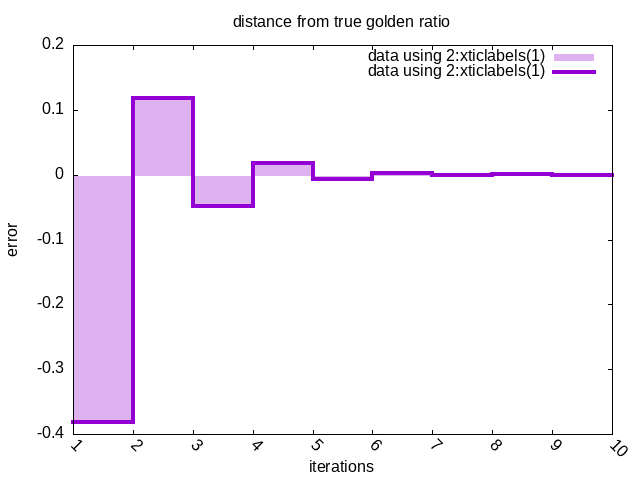
\includegraphics[width=.9\linewidth]{1/fig/1-36-1.png}
\end{center}

\(k\) must be at least 10 to get precision of 4 decimal places.

\subsubsection{Question C}
\label{sec:orga67031b}

\begin{quote}
If your \texttt{cont-frac} procedure generates a recursive process, write one that
generates an iterative process. If it generates an iterative process, write one
that generates a recursive process.
\end{quote}

\subsubsection{Answer C}
\label{sec:org155e7ae}
\begin{minted}[breaklines=true,breakanywhere=true,linenos=true]{scheme}
(define (cont-frac-rec n d k)
  (define (rec i)
    (if (= i k)
        (/ (n i) (d i))
        (/ (n i) (+ (d i) (rec (1+ i))))))

  (rec 1))
\end{minted}
\begin{minted}[breaklines=true,breakanywhere=true,linenos=true]{scheme}
<<cont-frac>>
<<cont-frac-rec>>
(define (golden-ratio k)
  (cont-frac (λ(i) 1.0)(λ(i)1.0) k))
(define (golden-ratio-rec k)
  (cont-frac-rec (λ(i) 1.0)(λ(i)1.0) k))

(load "mattcheck.scm")
(mattcheck-equal "cont-frac iter and recursive equivalence"
           (golden-ratio-rec 15)
           (golden-ratio 15))
\end{minted}

\begin{verbatim}
SUCCEED at cont-frac iter and recursive equivalence
\end{verbatim}

\subsection{Exercise 1.38}
\label{sec:orgff11c5a}
\subsubsection{Question}
\label{sec:org2e838a1}
\begin{quote}
In 1737, the Swiss mathematician Leonhard Euler published a memoir \emph{De
Fractionibus Continuis}, which included a continued fraction expansion for \(e -
2\), where \(e\) is the base of the natural logarithms. In this fraction, the
\(N_i\) are all 1, and the \(D_i\) are successively 1, 2, 1, 1, 4, 1, 1, 6, 1,
1, 8, \(\dots\). Write a program that uses your \texttt{cont-frac} procedure from
Exercise 1.37 to approximate \(e\), based on Euler's expansion.
\end{quote}
\subsubsection{Answer}
\label{sec:org2845142}
\begin{minted}[breaklines=true,breakanywhere=true,linenos=true]{scheme}
<<cont-frac>>
(define (euler k)
  (+ 2
     (cont-frac (λ(i) 1.0)
             (λ(i) (let ((j (1+ i)))
                     (if (= 0 (modulo j 3))
                         (* 2 (/ j 3))
                         1)))
             k)))

(euler 100)
\end{minted}

\begin{verbatim}
2.7182818284590455
\end{verbatim}

\subsection{Exercise 1.39}
\label{sec:orgb8390ea}
\subsubsection{Question}
\label{sec:orgba69be1}
\begin{quote}
A continued fraction representation of the tangent function was published in
1770 by the German mathematician J.H. Lambert:

\[ {\tan x} = \cfrac{x}{1 - \cfrac{x^2}{3 - \cfrac{x^2}{5 - \dots}}} \]

where \(x\) is in radians. Define a procedure \mintinline[breaklines=true,breakanywhere=true,linenos=true]{scheme}{(tan-cf x k)} that
computes an approximation to the tangent function based on Lambert's formula.
\texttt{k} specifies the number of terms to compute, as in Exercise 1.37.
\end{quote}
\subsubsection{Answer}
\label{sec:orgfb355ce}
\begin{minted}[breaklines=true,breakanywhere=true,linenos=true]{scheme}
<<cont-frac>>
(define (tan-cf x k)
  (cont-frac (λ(i) (if (= i 1)
                       x
                       (* x x -1.0)))
             (λ(i) (if (= i 1)
                       1.0
                       (- (* i 2.0) 1.0)))
             k))

(tan-cf 55 101)
\end{minted}

\begin{verbatim}
-45.1830879105221
\end{verbatim}
\subsection{1.3.4 Procedures as Returned Values}
\label{sec:orge182831}
Procedures can return other procedures, which opens up new ways to express
processes.

\begin{quote}
Newton's Method: \(g(x)=0\) is a fixed point of the function \(x \mapsto f(x)\)
where \[f(x)=x-\frac{g(x)}{Dg(x)}\]

Where \(x \mapsto g(x)\) is a differentiable function and \(Dg(x)\) is the
derivative of \(g\) evaluated at \(x\).
\end{quote}
\subsection{Exercise 1.40}
\label{sec:orge5d0b33}
\subsubsection{Text}
\label{sec:orge9c612b}
\begin{minted}[breaklines=true,breakanywhere=true,linenos=true]{scheme}
(define (average-damp f)
  (lambda (x) (average x (f x))))
\end{minted}

\begin{minted}[breaklines=true,breakanywhere=true,linenos=true]{scheme}
(define dx 0.00001)
\end{minted}

\begin{minted}[breaklines=true,breakanywhere=true,linenos=true]{scheme}
(define (deriv g)
  (lambda (x) (/ (- (g (+ x dx)) (g x)) dx)))
\end{minted}

\begin{minted}[breaklines=true,breakanywhere=true,linenos=true]{scheme}
(define (newton-transform g)
  (lambda (x) (- x (/ (g x) ((deriv g) x)))))
(define (newtons-method g guess)
  (fixed-point (newton-transform g) guess))
\end{minted}
\begin{minted}[breaklines=true,breakanywhere=true,linenos=true]{scheme}
<<average>>
<<average-damp>>
<<dx>>
<<deriv>>
<<newtons-method>>
\end{minted}
\subsubsection{Question}
\label{sec:org98f0e50}
\begin{quote}
Define a procedure \texttt{cubic} that can be used together with the \texttt{newtons-method}
procedure in expressions of the form:
\end{quote}

\begin{minted}[breaklines=true,breakanywhere=true,linenos=true]{scheme}
(newtons-method (cubic a b c) 1)
\end{minted}

\begin{quote}
to approximate zeros of the cubic \(x^3 + ax^2 + bx + c\).
\end{quote}
\subsubsection{Answer}
\label{sec:org32265eb}
\begin{minted}[breaklines=true,breakanywhere=true,linenos=true]{scheme}
(define (cubic a b c)
  (lambda (x)
    (+ (expt x 3)
       (* a (expt x 2))
       (* b x)
       c)))
\end{minted}

\begin{minted}[breaklines=true,breakanywhere=true,linenos=true]{scheme}
(define (cubic-zero a b c)
  (newtons-method (cubic a b c) 1))
\end{minted}

\begin{minted}[breaklines=true,breakanywhere=true,linenos=true]{scheme}
<<fixed-point-txt>>
<<newtons-method-txt>>
<<cubic>>
<<cubic-zero>>

(cubic-zero 2 3 4)
\end{minted}

\subsection{Exercise 1.41}
\label{sec:org9d993ee}
\subsubsection{Question}
\label{sec:org4bd3c2e}
\begin{quote}
Define a procedure \texttt{double} that takes a procedure of one argument as argument
and returns a procedure that applies the original procedure twice. For example,
if \texttt{inc} is a procedure that adds 1 to its argument, then \mintinline[breaklines=true,breakanywhere=true,linenos=true]{scheme}{(double inc)}
should be a procedure that adds 2. What value is returned by
\end{quote}

\begin{minted}[breaklines=true,breakanywhere=true,linenos=true]{scheme}
(((double (double double)) inc) 5)
\end{minted}

\subsubsection{Answer}
\label{sec:orgd58b7fa}
\begin{minted}[breaklines=true,breakanywhere=true,linenos=true]{scheme}
(define (double f)
  (λ (x)
    (f (f x))))
\end{minted}

\begin{minted}[breaklines=true,breakanywhere=true,linenos=true]{scheme}
(define inc 1+)
<<double>>
<<Ex1-41>>
\end{minted}

\begin{verbatim}
21
\end{verbatim}

\subsection{Exercise 1.42}
\label{sec:org18afa5b}
\subsubsection{Question}
\label{sec:org4fd88f0}
\begin{quote}
Let \(f\) and \(g\) be two one-argument functions. The composition \(f\) after
\(g\) is defined to be the function \(x \mapsto f(g(x))\). Define a procedure
\texttt{compose} that implements composition.
\end{quote}

\subsubsection{Answer}
\label{sec:org7f365eb}
\begin{minted}[breaklines=true,breakanywhere=true,linenos=true]{scheme}
(define (compose f g)
  (λ(x)
    (f (g x))))
\end{minted}

\begin{minted}[breaklines=true,breakanywhere=true,linenos=true]{scheme}
<<compose>>
<<square>>
(define inc 1+)
((compose square inc) 6)
\end{minted}

\begin{verbatim}
49
\end{verbatim}

\subsection{Exercise 1.43}
\label{sec:org565894b}
\subsubsection{Question}
\label{sec:orgecf051f}
\begin{quote}
If \(f\) is a numerical function
and \(n\) is a positive integer, then we can form the \(n^{\mathrm{th}}\) repeated
application of \(f\), which is defined to be the function whose value at \(x\)
is \(f(f(\dots (f(x))\dots ))\).  For example, if \(f\) is the
function \(x \mapsto x + 1\), then the \(n^{\mathrm{th}}\) repeated application of \(f\) is
the function \(x \mapsto x + n\).  If \(f\) is the operation of squaring a
number, then the \(n^{\mathrm{th}}\) repeated application of \(f\) is the function that
raises its argument to the \(2^n\)-th power.  Write a procedure that takes as
inputs a procedure that computes \(f\) and a positive integer \(n\) and returns
the procedure that computes the \(n^{\mathrm{th}}\) repeated application of \(f\).
\end{quote}

\subsubsection{Answer}
\label{sec:orgf46f7ad}
\begin{minted}[breaklines=true,breakanywhere=true,linenos=true]{scheme}
<<compose>>
(define (repeated f n)
  (if (= n 1)
      f
      (repeated (compose f f)
                (- n 1))))
\end{minted}

\begin{minted}[breaklines=true,breakanywhere=true,linenos=true]{scheme}
<<square>>
<<repeated>>
(if (= ((repeated square 2) 5) 625)
    "Success"
    "Fail")
\end{minted}

\begin{verbatim}
Success
\end{verbatim}

\subsection{Exercise 1.44}
\label{sec:org668f968}
\subsubsection{Question}
\label{sec:org44476d3}
\index{smoothing}
\begin{quote}
The idea of smoothing a function is an important concept in signal processing.
If \(f\) is a function and \(dx\) is some small number, then the smoothed
version of \(f\) is the function whose value at a point \(x\) is the average of
\(f(x - dx)\), \(f(x)\), and \(f(x + dx)\). Write a procedure \texttt{smooth} that
takes as input a procedure that computes \(f\) and returns a procedure that
computes the smoothed \(f\). It is sometimes valuable to repeatedly smooth a
function (that is, smooth the smoothed function, and so on) to obtain the
\(n\)-fold smoothed function. Show how to generate the \(n\)-fold smoothed
function of any given function using \texttt{smooth} and \texttt{repeated} from Exercise 1.43.
\end{quote}
\subsubsection{Answer}
\label{sec:orgc01c864}
\begin{minted}[breaklines=true,breakanywhere=true,linenos=true]{scheme}
<<average-varargs>>
(define (smooth f)
  (λ(x)
    (average (f (- x dx))
             (f x)
             (f (+ x dx)))))
(define (smooth-n f n)
  ((repeated smooth n) f))
\end{minted}

\subsection{Exercise 1.45}
\label{sec:orga5731df}
\subsubsection{Question}
\label{sec:orgd474fe4}
\begin{quote}
We saw in 1.3.3 that attempting to compute square roots by naively finding a
fixed point of \(y \mapsto x / y\) does not converge, and that this can be fixed by
average damping. The same method works for finding cube roots as fixed points of
the average-damped \(y \mapsto x / y^2\). Unfortunately, the process does not work for
fourth roots---a single average damp is not enough to make a fixed-point search
for \(y \mapsto x / y^3\) converge. On the other hand, if we average damp twice (i.e.,
use the average damp of the average damp of \(y \mapsto x / y^3\)) the fixed-point
search does converge. Do some experiments to determine how many average damps
are required to compute \(n^{\mathrm{th}}\) roots as a fixed-point search based
upon repeated average damping of \(y \mapsto x / y^{n-1}\). Use this to implement a
simple procedure for computing \(n^{\mathrm{th}}\) roots using \texttt{fixed-point},
\texttt{average-damp}, and the \texttt{repeated} procedure of Exercise 1.43. Assume that any
arithmetic operations you need are available as primitives.
\end{quote}
\subsubsection{Answer}
\label{sec:org9e2b724}
So this is strange. Back in my original workthrough of this book, I'd decided
that finding an \(n\)th root required \(\lfloor\sqrt{n}\rfloor\) dampings. With
a solution like this:
\begin{minted}[breaklines=true,breakanywhere=true,linenos=true]{scheme}
<<fixed-point-txt>>
<<repeated>>
<<average-damp>>
(define (sqrt n)
  (fixed-point
   (average-damp
    (lambda (y)
      (/ x y)))
   1.0))
(define (nth-root x n)
  (fixed-point
   ((repeated average-damp (ceiling (sqrt n)))
    (lambda (y)
      (/ x (expt y (- n 1)))))
   1.0))
\end{minted}
While this solution appears to work fine, my experiments are suggesting that it
takes \emph{less} than \(\lfloor\sqrt{n}\rfloor\). For example, I originally thought
powers of 16 required four dampings, but this code isn't failing until it
reaches powers of 32.
\begin{minted}[breaklines=true,breakanywhere=true,linenos=true]{scheme}
;; Version of "repeated" that can handle being asked to repeat zero times.
<<compose>>
<<identity>>
(define (repeated f n)
  (define (rec m)
  (if (= n 1)
      f
      (repeated (compose f f)
                (- n 1))))
  (if (= n 0)
      identity
      (rec n)))
\end{minted}
\begin{minted}[breaklines=true,breakanywhere=true,linenos=true]{scheme}
;; version of "fixed-point" that will give up after a certain number of guesses.
(define (limited-fixed-point f first-guess)
  (define limit 5000)
  (define tolerance 0.00000001)
  (define (close-enough? v1 v2)
    (< (abs (- v1 v2)) 
       tolerance))
  (define (try guess tries)
    (if (= tries limit)
        "LIMIT REACHED"
        (let ((next (f guess)))
          (if (close-enough? guess next)
              next
              (try next (+ 1 tries))))))
    (try first-guess 1))
\end{minted}
Let's automatically find how many dampings are necessary. We can make a program
that finds higher and higher \(n\)th roots, and adds another layer of damping
when it hits the error. It returns a list of \(n\)th roots along with how many
dampings were needed to find them.

\begin{minted}[breaklines=true,breakanywhere=true,linenos=true]{scheme}
<<fixed-point-txt>>
<<limited-fixed-point>>
<<repeated>>
<<average-damp>>
<<average>>
<<print-table>>
(define (sqrt x)
  (fixed-point
   (average-damp
    (lambda (y) (/ x y)))
   1.0))
(define (nth-tester base n-max)
  (define (iter ll)
    (let ((n (+ 2 (length ll))))
      (define (try damps)
        (let ((x (limited-fixed-point
                  ((repeated average-damp damps)
                   (lambda (y)
                     (/ base (expt y (- n 1)))))
                  1.1)))
          (if (string? x)
              (try (1+ damps))
              (list base n x damps))))
      (if (> n n-max)
          ll
          (iter (cons (try 1) ll)))))

  (iter '()))
(let* ((t (reverse (nth-tester 3 65))))
  (cons '("root" "result" "damps needed" "floor(sqrt(root))" "floor(log2(root))")
        (map (λ(x)
               (append x
                       (list (floor (sqrt (car x)))
                             (floor (/ (log (car x))(log 2))))))
             (map cdr t))))
\end{minted}

\begin{center}
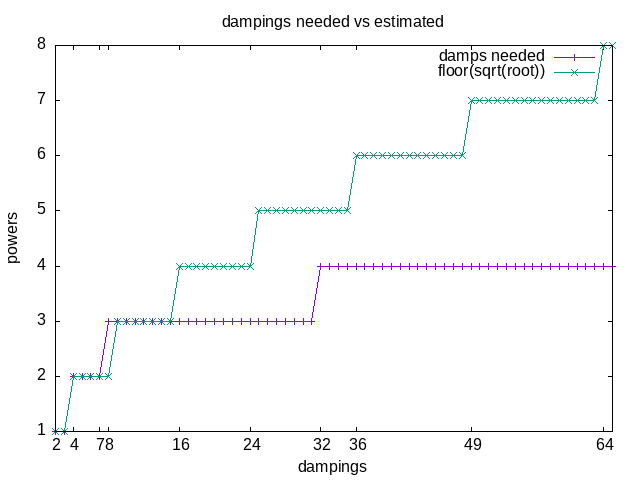
\includegraphics[width=.9\linewidth]{1/fig/1-45-1.png}
\end{center}

I've spent too much time on this problem already but I have to wonder about
floating-point issues, given that they are the core of the \texttt{good-enough}
procedure. I have to wonder whether a \texttt{fixed-point} version that replaces the
\texttt{tolerance} decision making, and instead retains the last three guesses and
checks for a loop.

\subsection{Exercise 1.46}
\label{sec:orgebe9a5a}
\subsubsection{Question}
\label{sec:orgc22f146}
\begin{quote}
Several of the numerical methods described in this chapter are instances of an
extremely general computational strategy known as \emph{iterative improvement}.
Iterative improvement says that, to compute something, we start with an initial
guess for the answer, test if the guess is good enough, and otherwise improve
the guess and continue the process using the improved guess as the new guess.
Write a procedure \texttt{iterative-improve} that takes two procedures as arguments: a
method for telling whether a guess is good enough and a method for improving a
guess. \texttt{iterative-improve} should return as its value a procedure that takes a
guess as argument and keeps improving the guess until it is good enough. Rewrite
the \texttt{sqrt} procedure of 1.1.7 and the \texttt{fixed-point} procedure of 1.3.3 in terms
of \texttt{iterative-improve}.
\end{quote}
\subsubsection{Answer}
\label{sec:org395008d}
\begin{minted}[breaklines=true,breakanywhere=true,linenos=true]{scheme}
(define (iterative-improve good-enough? improve)
  (λ(first-guess)
    (define (iter guess)
      (let ((next (improve guess)))
        (if (good-enough? guess next)
            next
            (iter next))))
    (iter first-guess)))
\end{minted}
\begin{minted}[breaklines=true,breakanywhere=true,linenos=true]{scheme}
<<iterative-improve>>
(define tolerance 0.00001)

(define (fixed-point-improve f first-guess)
  (define (close-enough? v1 v2)
    (< (abs (- v1 v2)) 
       tolerance))
  ((iterative-improve close-enough? f) first-guess))
\end{minted}
\begin{minted}[breaklines=true,breakanywhere=true,linenos=true]{scheme}
<<average>>
<<iterative-improve>>
(define (improve guess x)
  (average guess (/ x guess)))
(define (good-enough? guess x)
   (= (improve guess x) guess))
(define (sqrt-improve x)
  ((iterative-improve
    (λ(guess) (improve guess x))
    (λ(guess) (good-enough? guess x)))
   1.0))
\end{minted}


\begin{minted}[breaklines=true,breakanywhere=true,linenos=true]{scheme}
(load "mattcheck2.scm")
<<fixed-point-txt>>
<<fixed-point-improve>>
(mattcheck "fixed-point-improve still working"
                 (fixed-point (λ(x)(+ 1 (/ 1 x))) 1.0)
                 (fixed-point-improve (λ(x)(+ 1 (/ 1 x))) 1.0))
<<sqrt>>
<<sqrt-improve>>
(mattcheck "sqrt-improve still working"
                 (sqrt 5)
                 (sqrt 5))
\end{minted}

\begin{verbatim}
SUCCEED at fixed-point-improve still working
SUCCEED at sqrt-improve still working
\end{verbatim}

\section{Chapter 2: Building Abstractions with Data}
\label{sec:org380ffc7}
The basic representations of data we've used so far aren't enough to deal with
complex, real-world phenomena. We need to combine these representations to form
\textbf{compound data}.

The technique of isolating how data objects are \emph{represented} from how they are
\emph{used} is called \textbf{data abstraction}.

\subsection{2.1.1: Example: Arithmetic Operations for Rational Numbers}
\label{sec:orgb4b71d1}
Lisp gives the procedures \texttt{cons}, \texttt{car}, and \texttt{cdr} to create \textbf{pairs}. This is an
easy system for representing rational numbers.

Note that the system proposed for representing and working with rational numbers
has \textbf{abstraction barriers} isolating different parts of the system. The parts
that use rational numbers don't know how the constructors and selectors for
rational numbers work, and the constructors and selectors use the underlying
Lisp interpreter's pair functions without caring how they work.

Note that these abstraction layers allow the developer to change the underlying
architecture without modifying the programs that depend on it.

\subsection{Exercise 2.1}
\label{sec:orgcef0043}
\subsubsection{Text}
\label{sec:orgb299a0a}
\begin{minted}[breaklines=true,breakanywhere=true,linenos=true]{scheme}
(define (add-rat x y)
  (make-rat (+ (* (numer x) (denom y))
               (* (numer y) (denom x)))
            (* (denom x) (denom y))))

(define (sub-rat x y)
  (make-rat (- (* (numer x) (denom y))
               (* (numer y) (denom x)))
            (* (denom x) (denom y))))

(define (mul-rat x y)
  (make-rat (* (numer x) (numer y))
            (* (denom x) (denom y))))

(define (div-rat x y)
  (make-rat (* (numer x) (denom y))
            (* (denom x) (numer y))))

(define (equal-rat? x y)
  (= (* (numer x) (denom y))
     (* (numer y) (denom x))))
\end{minted}

\begin{minted}[breaklines=true,breakanywhere=true,linenos=true]{scheme}
(define (make-rat n d) (cons n d))
(define (numer x) (car x))
(define (denom x) (cdr x))
\end{minted}

\begin{minted}[breaklines=true,breakanywhere=true,linenos=true]{scheme}
(define (print-rat x)
  (newline)
  (display (numer x))
  (display "/")
  (display (denom x)))
\end{minted}

\begin{minted}[breaklines=true,breakanywhere=true,linenos=true]{scheme}
(define one-half (make-rat 1 2))
(define one-third (make-rat 1 3))
(print-rat one-half)
(print-rat
 (mul-rat one-half one-third))
\end{minted}
\begin{verbatim}
1/2
1/6
\end{verbatim}

\subsubsection{Question}
\label{sec:orge361f8b}
\begin{quote}
Define a better version of \texttt{make-rat} that handles both positive and negative
arguments. \texttt{make-rat} should normalize the sign so that if the rational number
is positive, both the numerator and denominator are positive, and if the
rational number is negative, only the numerator is negative.
\end{quote}

\subsubsection{Answer}
\label{sec:org953f2e5}
\begin{minted}[breaklines=true,breakanywhere=true,linenos=true]{scheme}
<<abs>>
(define (make-rat n d)
  (cond ((not (or (< n 0)
              (< d 0)))
         (cons n d))
        ((and (< n 0)
              (< d 0))
         (cons (- n) (- d)))
        (else
         (cons (- (abs n)) (abs d)))))
(define (numer x) (car x))
(define (denom x) (cdr x))

;; Bonus: an attempt to optimize
(define (make-rat-opt n d)
  (let ((nn (< n 0))
        (dn (< d 0)))
    (cond ((not (or nn dn))
           (cons n d))
          ((and nn dn)
           (cons (- n) (- d)))
          (else
           (cons (- (abs n)) (abs d))))))
\end{minted}
\begin{minted}[breaklines=true,breakanywhere=true,linenos=true]{scheme}
<<make-rat>>
<<print-rat-txt>>
<<rat-ops-txt>>
(load "mattcheck2.scm")
(mattcheck "make-rat double negative"
           (cons 1 2)
           (make-rat -1 -2))
(mattcheck "make-rat numerator negative"
           (cons -1 2)
           (make-rat -1 2))
(mattcheck "make-rat denominator negative"
           (cons -1 2)
           (make-rat 1 -2))
(mattcheck "make-rat-opt double negative"
           (cons 1 2)
           (make-rat-opt -1 -2))
(mattcheck "make-rat-opt numerator negative"
           (cons -1 2)
           (make-rat-opt -1 2))
(mattcheck "make-rat-opt denominator negative"
           (cons -1 2)
           (make-rat-opt 1 -2))
\end{minted}

\begin{verbatim}
SUCCEED at make-rat double negative
SUCCEED at make-rat numerator negative
SUCCEED at make-rat denominator negative
SUCCEED at make-rat-opt double negative
SUCCEED at make-rat-opt numerator negative
SUCCEED at make-rat-opt denominator negative
\end{verbatim}

My ``optimized'' version shows no benefit at all:
\begin{verbatim}
unoptimized make-rat: ((1 . 2) 231.74267794)
optimized make-rat: ((1 . 2) 233.99087033)
\end{verbatim}
\subsection{Exercise 2.2}
\label{sec:org2b440cf}
\subsubsection{Question}
\label{sec:org93e03b3}
Consider the problem of representing line segments in a plane. Each segment is
represented as a pair of points: a starting point and an ending point. Define a
constructor \texttt{make-segment} and selectors \texttt{start-segment} and \texttt{end-segment} that
define the representation of segments in terms of points. Furthermore, a point
can be represented as a pair of numbers: the \(x\) coordinate and the \(y\)
coordinate. Accordingly, specify a constructor \texttt{make-point} and selectors
\texttt{x-point} and \texttt{y-point} that define this representation. Finally, using your
selectors and constructors, define a procedure \texttt{midpoint-segment} that takes a
line segment as argument and returns its midpoint (the point whose coordinates
are the average of the coordinates of the endpoints). To try your procedures,
you'll need a way to print points:

\begin{minted}[breaklines=true,breakanywhere=true,linenos=true]{scheme}
(define (print-point p)
  (newline)
  (display "(")
  (display (x-point p))
  (display ",")
  (display (y-point p))
  (display ")"))
\end{minted}
\subsubsection{Answer}
\label{sec:orgf640817}
\begin{minted}[breaklines=true,breakanywhere=true,linenos=true]{scheme}
<<average>>
(define (make-point x y)
  (cons x y))
(define (x-point p)
  (car p))
(define (y-point p)
  (cdr p))
(define (make-segment start end)
  (cons start end))
(define (start-segment seg)
  (car seg))
(define (end-segment seg)
  (cdr seg))
(define (midpoint-segment seg)
  (make-point (average (x-point (start-segment seg))
                       (x-point (end-segment seg)))
              (average (y-point (start-segment seg))
                       (y-point (end-segment seg)))))
(define (midpoint-segment-opt seg)
  (let ((ax (x-point (start-segment seg)))
        (bx (x-point (end-segment seg)))
        (ay (y-point (start-segment seg)))
        (by (y-point (end-segment seg))))
  (make-point (average ax
                       bx)
              (average ay
                       by))))
\end{minted}
\begin{minted}[breaklines=true,breakanywhere=true,linenos=true]{scheme}
<<make-point>>
(load "mattcheck2.scm")
(mattcheck "make-point"
           (list 1 2)
           (let ((p (make-point 1 2)))
             (list (x-point p)
                   (y-point p))))
(let* ((p1 (make-point 1 2))
      (p2 (make-point -1 -2))
      (s (make-segment p1 p2)))
  (mattcheck "make-segment"
             (list p1 p2)
             (list (start-segment s)
                   (end-segment s)))
  (mattcheck "midpoint-segment"
              (make-point 0 0)
              (midpoint-segment s))
  (mattcheck "midpoint-segment-opt"
              (make-point 0 0)
              (midpoint-segment-opt s)))
\end{minted}

\begin{verbatim}
SUCCEED at make-point
SUCCEED at make-segment
SUCCEED at midpoint-segment
SUCCEED at midpoint-segment-opt
\end{verbatim}

And once again my bikeshedding is revealed:
\begin{verbatim}
unoptimized make-rat: ((0.0 . 0.0) 326.94653558)
optimized make-rat: ((0.0 . 0.0) 331.83410742)
\end{verbatim}

\subsection{Exercise 2.3}
\label{sec:org0ea0bd1}
\subsubsection{Question}
\label{sec:org8062572}
Implement a representation for rectangles in a plane. (Hint: You may want to
make use of Exercise 2.2.) In terms of your constructors and selectors, create
procedures that compute the perimeter and the area of a given rectangle. Now
implement a different representation for rectangles. Can you design your system
with suitable abstraction barriers, so that the same perimeter and area
procedures will work using either representation?
\subsubsection{Answer 1}
\label{sec:orgf8ab97d}
I don't really like the ``wishful thinking'' process the book advocates but since
this question specifically regards abstraction, I'll start by writing the two
requested procedures first.

\begin{minted}[breaklines=true,breakanywhere=true,linenos=true]{scheme}
(define (rect-area R)
  (* (rect-height R)
     (rect-width R)))

(define (rect-peri R)
  (* 2
     (+ (rect-height R)
        (rect-width R))))
\end{minted}

So my ``wishlist'' is just for \mintinline[breaklines=true,breakanywhere=true,linenos=true]{scheme}{(rect-area R)} and \mintinline[breaklines=true,breakanywhere=true,linenos=true]{scheme}{(rect-width R)}.

So, my first implementation of a rectangle will be of a list of 3 points
\(\mathrm{ABC}\), with the fourth point \(\mathrm{D}\) being constructed from
the others. I haven't done geometry lessons in a while but logically I can
deduce that \(\mathrm{D}\) is as far from \(\mathrm{A}\) as \(\mathrm{B}\) is
from \(\mathrm{C}\), and as far from \(\mathrm{C}\) as \(\mathrm{A}\) is from
\(\mathrm{B}\). by experimentation I've figured out that
\(\mathrm{D}=\mathrm{A} + (\mathrm{C}-\mathrm{B})=\mathrm{C} +
(\mathrm{A}-\mathrm{B})\).

\begin{minted}[breaklines=true,breakanywhere=true,linenos=true]{scheme}
;;   AB = width
;;(0,1) (1,1)
;; A-----B
;; |     | BC = height
;; D-----C
;;(0,0) (1,0)
;; could be rotated any direction
<<square>>
<<make-point>>
(define (make-rect a b c)
  (cons (cons a b) c))
(define (rect-a R)
  (caar R))
(define (rect-b R)
  (cdar R))
(define (rect-c R)
  (cdr R))
;(define (rect-d R)
;  (make-point (x-point (rect-a R))
;              (y-point (rect-c R))))
;; Wait, this won't work if the rectangle is angled.

(define (sub-points a b)
  (make-point (- (x-point a)
                 (x-point b))
              (- (y-point a)
                 (y-point b))))

(define (add-points a b)
  (make-point (+ (x-point a)
                 (x-point b))
              (+ (y-point a)
                 (y-point b))))

(define (rect-d R)
  (let ((a (rect-a R))
        (b (rect-b R))
        (c (rect-c R)))
    (add-points a
                (sub-points c b))))
(define (rect-d-alt R) ; should be mathematically identical.
  (let ((a (rect-a R))
        (b (rect-b R))
        (c (rect-c R)))
    (add-points c
                (sub-points a b))))

;; this is incorrect
;(define (length-points a b)
;  (let ((diffP (sub-points a b)))
;    (+ (abs (x-point diffP))
;       (abs (y-point diffP)))))
(define (length-points a b)
  (let ((ax (x-point a))
        (ay (y-point a))
        (bx (x-point b))
        (by (y-point b)))
    (sqrt (+ (square (- ax bx))
          (square (- ay by))))))

(define (rect-height R)
  (abs (length-points (rect-b R)
                 (rect-c R))))
(define (rect-width R)
  (abs (length-points (rect-b R)
                 (rect-a R))))

(define (length-segment seg)
  (abs (length-points (start-segment seg)
                 (end-segment seg))))
\end{minted}

\begin{minted}[breaklines=true,breakanywhere=true,linenos=true]{scheme}
(load "mattcheck2.scm")

<<rect-4pt>>
<<rect-area-peri>>

(let* ((a (make-point 13 14))
       (b (make-point 14 14))
       (c (make-point 14 13))
       (d (make-point 13 13))
       (ABC (make-rect a b c))
       (CDA (make-rect c d a))
       (w (make-point -2.0 -2.0))
       (x (make-point -0.5 -0.5))
       (y (make-point -1.5 0.5))
       (z (make-point -3.0 -1.0))
       (WXY (make-rect w x y)))
  (mattcheck "make-rect"
             ABC
             (cons (cons a b) c))
  (mattcheck "rect-d and rect-d-alt (ABCD)"
             (rect-d ABC)
             (rect-d-alt ABC)
             d)
  (mattcheck "rect-d and rect-d-alt (CDAB)"
             (rect-d CDA)
             (rect-d-alt CDA)
             b)
  (mattcheck "rect-d and rect-d-alt (WXYZ)"
             (rect-d WXY)
             (rect-d-alt WXY)
             z)
  (mattcheck "rect-d and rect-d-alt (XYZW)"
             (rect-d (make-rect x y z))
             w)
  (mattcheck "rect-height ABC"
             (rect-height ABC)
             1)
  (mattcheck "rect-width ABC"
             (rect-width ABC)
             1)
  (mattcheck "rect-height WXY"
             (rect-height WXY)
             1.4142135623730951)
  (mattcheck "rect-width WXY"
             (rect-width WXY)
             2.1213203435596424)
  (mattcheck "rect-area ABCD"
             (rect-area ABC)
             (rect-area CDA)
             1)
  (mattcheck "rect-area WXYZ"
             (rect-area WXY)
             3.0)
  (mattcheck "rect-peri ABCD"
             (rect-peri ABC)
             4)
  (mattcheck "rect-peri WXYZ"
             (rect-peri WXY)
             7.0710678118654755))
\end{minted}

\begin{verbatim}
SUCCEED at make-rect
SUCCEED at rect-d and rect-d-alt (ABCD)
SUCCEED at rect-d and rect-d-alt (CDAB)
SUCCEED at rect-d and rect-d-alt (WXYZ)
SUCCEED at rect-d and rect-d-alt (XYZW)
SUCCEED at rect-height ABC
SUCCEED at rect-width ABC
SUCCEED at rect-height WXY
SUCCEED at rect-width WXY
SUCCEED at rect-area ABCD
SUCCEED at rect-area WXYZ
SUCCEED at rect-peri ABCD
SUCCEED at rect-peri WXYZ
\end{verbatim}

\subsubsection{Answer 2}
\label{sec:org2c4232f}
My second implementation will be of a rectangle as an origin, height, width, and
angle. Basically, height and width are two vectors originating from origin, with
width going straight right and height offset \(90\deg\) from width. Angle is
added during conversion from Polar to Cartesian coordinates. In relation to my
1st implementation, point D is where the origin is.
\begin{minted}[breaklines=true,breakanywhere=true,linenos=true]{scheme}
<<make-point>>
;; origin is a (make-point), hwa are floats
(define (make-rect origin height width angle)
  (cons (cons origin height)
        (cons width angle)))

(define (rect-origin R)
  (caar R))
(define rect-d rect-origin)
(define (rect-height R)
  (cdar R))
(define (rect-width R)
  (cadr R))
(define (rect-angle R)
  (cddr R))

;; I underestimated how much math this would take.
(define (add-points a b)
  (make-point (+ (x-point a)
                 (x-point b))
              (+ (y-point a)
                 (y-point b))))

(define pi (* 4 (atan 1.0)))
(define (radian deg)
  (* deg (/ pi 180.0)))
(define (vector-to-xy distance angle)
      ;; rect-c: (cos(Theta),sin(Theta)) * width
      (make-point (* (cos (radian angle))
                     distance)
                  (* (sin (radian angle))
                     distance)))
      ;; could also be rotated by 90 degrees just by using
      ;;   (-sin(Theta),cos(Theta)) * height
(define (rect-c R)
  (add-points
   (rect-origin R)
   (vector-to-xy (rect-width R) (rect-angle R))))
(define (rect-a R)
  (add-points
   (rect-origin R)
   (vector-to-xy (rect-height R)
                 (+ 90 (rect-angle R)))))
(define (rect-b R)
  (add-points
   (rect-origin R)
   (add-points
    (vector-to-xy (rect-width R) (rect-angle R))
    (vector-to-xy (rect-height R)
                  (+ 90 (rect-angle R))))))
\end{minted}

\begin{minted}[breaklines=true,breakanywhere=true,linenos=true]{scheme}
(load "mattcheck2.scm")

<<rect-ohwa>>
<<rect-area-peri>>

(let* ((a (make-point 13.0 14.0))
       (b (make-point 14.0 14.0))
       (c (make-point 14.0 13.0))
       (d (make-point 13.0 13.0))
       (ABC (make-rect d 1 1 0))
       (CDA (make-rect b 1 1 180))
       (w (make-point -2.0 -2.0))
       (x (make-point -2.5 1.5))
       (y (make-point -1.5 0.5))
       (z (make-point -3.0 -1.0))
       (wxy-height 1.4142135623730951)
       (wxy-width 2.1213203435596424)
       (WXY (make-rect z wxy-height wxy-width 45)))
  (mattcheck "make-rect"
             ABC
             (cons (cons d 1) (cons 1 0)))
  (mattcheck "rect-b (ABCD)"
             (rect-b ABC)
             b)
  (mattcheck "rect-b (CDAB)"
             (rect-b CDA)
             d)
  (mattcheck "rect-b (WXYZ)"
             (rect-b WXY)
             x)
  (mattcheck "rect-height"
             (rect-height WXY)
             wxy-height)
  (mattcheck "rect-width"
             (rect-width WXY)
             wxy-width)
  (mattcheck "rect-area ABCD"
             (rect-area ABC)
             (rect-area CDA)
             1)
  (mattcheck "rect-area WXYZ"
             (rect-area WXY)
             3.0)
  (mattcheck "rect-peri ABCD"
             (rect-peri ABC)
             4)
  (mattcheck "rect-peri WXYZ"
             (rect-peri WXY)
             7.0710678118654755))
\end{minted}

\begin{verbatim}
SUCCEED at make-rect
SUCCEED at rect-b (ABCD)
SUCCEED at rect-b (CDAB)
SUCCEED at rect-b (WXYZ)
SUCCEED at rect-height
SUCCEED at rect-width
SUCCEED at rect-area ABCD
SUCCEED at rect-area WXYZ
SUCCEED at rect-peri ABCD
SUCCEED at rect-peri WXYZ
\end{verbatim}

\subsection{2.1.3: What Is Meant by Data?}
\label{sec:orga971296}
We can consider data as being a collection of selectors and constructors,
together with specific conditions that these procedures must fulfill in order to
be a valid representation. For example, in the case of our rational number
implementation, for rational number \(x\) made with numerator \(n\) and
denominator \(d\), dividing the result of \mintinline[breaklines=true,breakanywhere=true,linenos=true]{scheme}{(numer x)} over the result
of \mintinline[breaklines=true,breakanywhere=true,linenos=true]{scheme}{(denom x)} should be equivalent to dividing \(n\) over \(d\).

\subsection{Exercise 2.4}
\label{sec:orga5338f8}
\subsubsection{Question}
\label{sec:org0a20371}
Here is an alternative procedural representation of pairs. For this
representation, verify that \mintinline[breaklines=true,breakanywhere=true,linenos=true]{scheme}{(car (cons x y))} yields \texttt{x} for any
objects \texttt{x} and \texttt{y}.

\begin{minted}[breaklines=true,breakanywhere=true,linenos=true]{scheme}
(define (cons x y)
  (lambda (m) (m x y)))
(define (car z)
  (z (lambda (p q) p)))
\end{minted}

What is the corresponding definition of \texttt{cdr}? (Hint: To verify that this works,
make use of the substitution model of 1.1.5.)

\subsubsection{Answer}
\label{sec:orgaabfc4b}
First, let's explain with the substitution model.
\begin{minted}[breaklines=true,breakanywhere=true,linenos=true]{scheme}
(cons 0 1)
(lambda (m) (m 0 1))

(car (lambda (m) (m 0 1)))
((lambda (m) (m 0 1)) (lambda (p q) p))
(lambda (0 1) 0)
0
(cdr (lambda (m) (m 0 1)))
((lambda (m) (m 0 1)) (lambda (p q) q))
(lambda (0 1) 1)
1
\end{minted}

Now for implementation.
\begin{minted}[breaklines=true,breakanywhere=true,linenos=true]{scheme}
(load "mattcheck2.scm")
<<alt-pairs-txt>>
(define (cdr z)
  (z (lambda (p q) q)))

(let ((pair (cons 0 1)))
  (mattcheck "car"
             (car pair)
             0)
  (mattcheck "cdr"
             (cdr pair)
             1))
\end{minted}

\begin{verbatim}
| (0 . 0) | (0 . 1) | (0 . 2) | (0 . 3) | (0 . 4) | (0 . 5) | (0 . 6) |
| (1 . 0) | (1 . 1) | (1 . 2) | (1 . 3) | (1 . 4) | (1 . 5) | (1 . 6) |
| (2 . 0) | (2 . 1) | (2 . 2) | (2 . 3) | (2 . 4) | (2 . 5) | (2 . 6) |
| (3 . 0) | (3 . 1) | (3 . 2) | (3 . 3) | (3 . 4) | (3 . 5) | (3 . 6) |
| (4 . 0) | (4 . 1) | (4 . 2) | (4 . 3) | (4 . 4) | (4 . 5) | (4 . 6) |
| (5 . 0) | (5 . 1) | (5 . 2) | (5 . 3) | (5 . 4) | (5 . 5) | (5 . 6) |
| (6 . 0) | (6 . 1) | (6 . 2) | (6 . 3) | (6 . 4) | (6 . 5) | (6 . 6) |
\end{verbatim}

\subsection{Exercise 2.5}
\label{sec:org6085a11}
\subsubsection{Question}
\label{sec:orgf45731b}
\begin{quote}
Show that we can represent pairs of nonnegative integers using only numbers and
arithmetic operations if we represent the pair \(a\) and \(b\) as the integer
that is the product \(2^a 3^b\). Give the corresponding definitions of the
procedures \texttt{cons}, \texttt{car}, and \texttt{cdr}.
\end{quote}
\subsubsection{Answer}
\label{sec:org922d2db}
This one really blew my mind inside-out when I first did it. Basically, because
the two numbers are coprime, you can factor out the unwanted number and be left
with the desired one.

\begin{quote}
Where \(x\) is the scrambled number, \(p\) is the base we want to remove, \(q\)
is the base we want to retrieve from and \(y\) is the value exponentiating
\(p\), the original number is retrieved by dividing \(x\) by \(p\) for \(y\)
number of times, and then applying \(\log_{q}\) to the result.
\end{quote}

First, let's make \texttt{cons}.
\begin{minted}[breaklines=true,breakanywhere=true,linenos=true]{scheme}
(define (cons-nnint a b)
  (* (expt 2 a) (expt 3 b)))
(define (cons-nnint-debug a b) ;; DEBUG
  (let* ((aa (expt 2 a))
         (bb (expt 3 b))
         (ab (* aa bb)))
    (display aa)
    (newline)
    (display bb)
    (newline)
    (display ab)
    (newline)
    ab))
\end{minted}

Also, Guile doesn't have a function for custom logs so let's define that now.
\begin{minted}[breaklines=true,breakanywhere=true,linenos=true]{scheme}
(define (logn b p)
  (/ (log p) (log b)))
\end{minted}

Let's do some analysis to see how these numbers are related.
\begin{minted}[breaklines=true,breakanywhere=true,linenos=true]{scheme}
<<cons-nnint>>
(let*
    ((tablesize 7)
     (inputs (map (λ(x)
                    (map (λ(y)
                           (cons x y))
                         (iota tablesize)))
                  (iota tablesize)))
     (outputs (map (λ(row)
                     (map (λ(col)
                            (cons-nnint (car col) (cdr col)))
                          row))
                   inputs)))
  outputs)
\end{minted}

\begin{center}
\begin{tabular}{rrrrrrr}
1 & 3 & 9 & 27 & 81 & 243 & 729\\
2 & 6 & 18 & 54 & 162 & 486 & 1458\\
4 & 12 & 36 & 108 & 324 & 972 & 2916\\
8 & 24 & 72 & 216 & 648 & 1944 & 5832\\
16 & 48 & 144 & 432 & 1296 & 3888 & 11664\\
32 & 96 & 288 & 864 & 2592 & 7776 & 23328\\
64 & 192 & 576 & 1728 & 5184 & 15552 & 46656\\
\end{tabular}
\end{center}

Here are our scrambled numbers. 

\begin{minted}[breaklines=true,breakanywhere=true,linenos=true]{scheme}
;; To find a number of some base in some column,
;; First divide by unwantedbase for targetcol number of times
<<repeated>>
(let ((targetcol 2)
      (unwantedbase 3))
  (map (λ(row)
         (map (λ(item)
                ((repeated (λ(x) 
                             (/ x unwantedbase)) targetcol)
                 item))
                row))
       data))
\end{minted}

\begin{center}
\begin{tabular}{llrrrrr}
1/9 & 1/3 & 1 & 3 & 9 & 27 & 81\\
2/9 & 2/3 & 2 & 6 & 18 & 54 & 162\\
4/9 & 4/3 & 4 & 12 & 36 & 108 & 324\\
8/9 & 8/3 & 8 & 24 & 72 & 216 & 648\\
16/9 & 16/3 & 16 & 48 & 144 & 432 & 1296\\
32/9 & 32/3 & 32 & 96 & 288 & 864 & 2592\\
64/9 & 64/3 & 64 & 192 & 576 & 1728 & 5184\\
\end{tabular}
\end{center}

The numbers from our target column onwards are integers, with the target column
being linearly exponentiated by 2 because the original numbers were linear.

\begin{minted}[breaklines=true,breakanywhere=true,linenos=true]{scheme}
<<logn>>
(let ((wantedbase 2))
  (map (λ(row)
         (map (λ(item)
                (format #f "~6,3f" (logn 2 item)))
                row))
       data))
\end{minted}

\begin{center}
\begin{tabular}{rrrrrrr}
-3.170 & -1.585 & 0.000 & 1.585 & 3.170 & 4.755 & 6.340\\
-2.170 & -0.585 & 1.000 & 2.585 & 4.170 & 5.755 & 7.340\\
-1.170 & 0.415 & 2.000 & 3.585 & 5.170 & 6.755 & 8.340\\
-0.170 & 1.415 & 3.000 & 4.585 & 6.170 & 7.755 & 9.340\\
0.830 & 2.415 & 4.000 & 5.585 & 7.170 & 8.755 & 10.340\\
1.830 & 3.415 & 5.000 & 6.585 & 8.170 & 9.755 & 11.340\\
2.830 & 4.415 & 6.000 & 7.585 & 9.170 & 10.755 & 12.340\\
\end{tabular}
\end{center}

Now the second column has recovered its original values. Although we didn't know
what the original integer values were, we can now tell which column has the
correct numbers by looking at which are integer values.

We can use this sign of a correct result in the proposed \texttt{car} and \texttt{cdr} procedures.

\begin{minted}[breaklines=true,breakanywhere=true,linenos=true]{scheme}
<<cons-nnint>>
<<logn>>
(use-srfis '(1))
(define (all-your-base ab unwanted wanted)
  (if (equal? (modulo ab unwanted) 0)
      (all-your-base (/ ab unwanted) unwanted wanted)
      (if (equal? (modulo ab wanted) 0)
          (round (logn wanted ab))
          "This number isn't a factor!")))
(define (car-nnint ab)
  (all-your-base ab 3 2))
(define (cdr-nnint ab)
  (all-your-base ab 2 3))

(let* ((initvalues '((2 3) (4 5) (7 2)))
       (conslist (map (λ(x)
                        (apply cons-nnint x))
                      initvalues))
       (carlist (map (λ(x)
                       (car-nnint x))
                     conslist))
       (cdrlist (map (λ(x)
                       (cdr-nnint x))
                     conslist)))
  (map (λ(x y) (cons x y))
       (list "pairs" "cons'd" "car" "cdr")
       (list initvalues conslist carlist cdrlist)))
\end{minted}

\begin{center}
\begin{tabular}{lrrr}
pairs & (2 3) & (4 5) & (7 2)\\
\hline
cons'd & 108 & 3888 & 1152\\
car & 2.0 & 4.0 & 7.0\\
cdr & 3.0 & 5.0 & 2.0\\
\end{tabular}
\end{center}

\subsection{Exercise 2.6}
\label{sec:orgad0cd11}
\subsubsection{Question}
\label{sec:orgb305f72}
\begin{quote}
In case representing pairs as procedures wasn't mind-boggling enough, consider
that, in a language that can manipulate procedures, we can get by without
numbers (at least insofar as nonnegative integers are concerned) by implementing
0 and the operation of adding 1 as
\end{quote}

\begin{minted}[breaklines=true,breakanywhere=true,linenos=true]{scheme}
(define zero (λ (f) (λ (x) x)))
(define (add-1 n)
  (λ (f) (λ (x) (f ((n f) x)))))
\end{minted}

\begin{quote}
This representation is known as \emph{Church numerals}, after its inventor, Alonzo
Church, the logician who invented the λ-calculus.

Define \mintinline[breaklines=true,breakanywhere=true,linenos=true]{scheme}{one} and \mintinline[breaklines=true,breakanywhere=true,linenos=true]{scheme}{two} directly (not in terms of
\mintinline[breaklines=true,breakanywhere=true,linenos=true]{scheme}{zero} and \mintinline[breaklines=true,breakanywhere=true,linenos=true]{scheme}{add-1}). (Hint: Use substitution to evaluate
\mintinline[breaklines=true,breakanywhere=true,linenos=true]{scheme}{(add-1 zero)}). Give a direct definition of the addition procedure
\mintinline[breaklines=true,breakanywhere=true,linenos=true]{scheme}{+} (not in terms of repeated application of \mintinline[breaklines=true,breakanywhere=true,linenos=true]{scheme}{add-1}).
\end{quote}

\subsubsection{Answer}
\label{sec:org0bd184f}
First, let's check out \mintinline[breaklines=true,breakanywhere=true,linenos=true]{scheme}{(add-1 zero)}.
\begin{minted}[breaklines=true,breakanywhere=true,linenos=true]{scheme}
(define zero (λ (f) (λ (x) x)))
(define (add-1 n)
  (λ (f) (λ (x)
           (f ((n f) x)))))

(add-1 zero)
((λ (f) (λ (x)
          (f ((zero f) x)))))
((λ (f) (λ (x)
          (f ((λ (x) x) x)))))
((λ (f) (λ (x)
          (f x))))
\end{minted}

So from this I believe the correct definition of one and two are:
\begin{minted}[breaklines=true,breakanywhere=true,linenos=true]{scheme}
(load "mattcheck2.scm")
(define one
  (λ (f) (λ (x)
           (f x))))
(define two
  (λ (f) (λ (x)
            (f (f x)))))

(mattcheck "1 = 1+0"
           1
           ((one 1+) 0))
(mattcheck "2 = 1+1+0"
           2
           ((two 1+) 0))

(define (add a b)
  (λ (f) (λ (x)
           ((a f) ((b f) x)))))

(mattcheck "3 = 1+2 = (1+0) + (1+1+0)"
           3
           (((add one two) 1+) 0))
\end{minted}

\begin{verbatim}
SUCCEED at 1 = 1+0
SUCCEED at 2 = 1+1+0
SUCCEED at 3 = 1+2 = (1+0) + (1+1+0)
\end{verbatim}

\subsection{2.2: Hierarchical Data and the Closure Property}
\label{sec:org9ee882f}
\texttt{cons} pairs can be used to construct more complex data-types.

\begin{center}
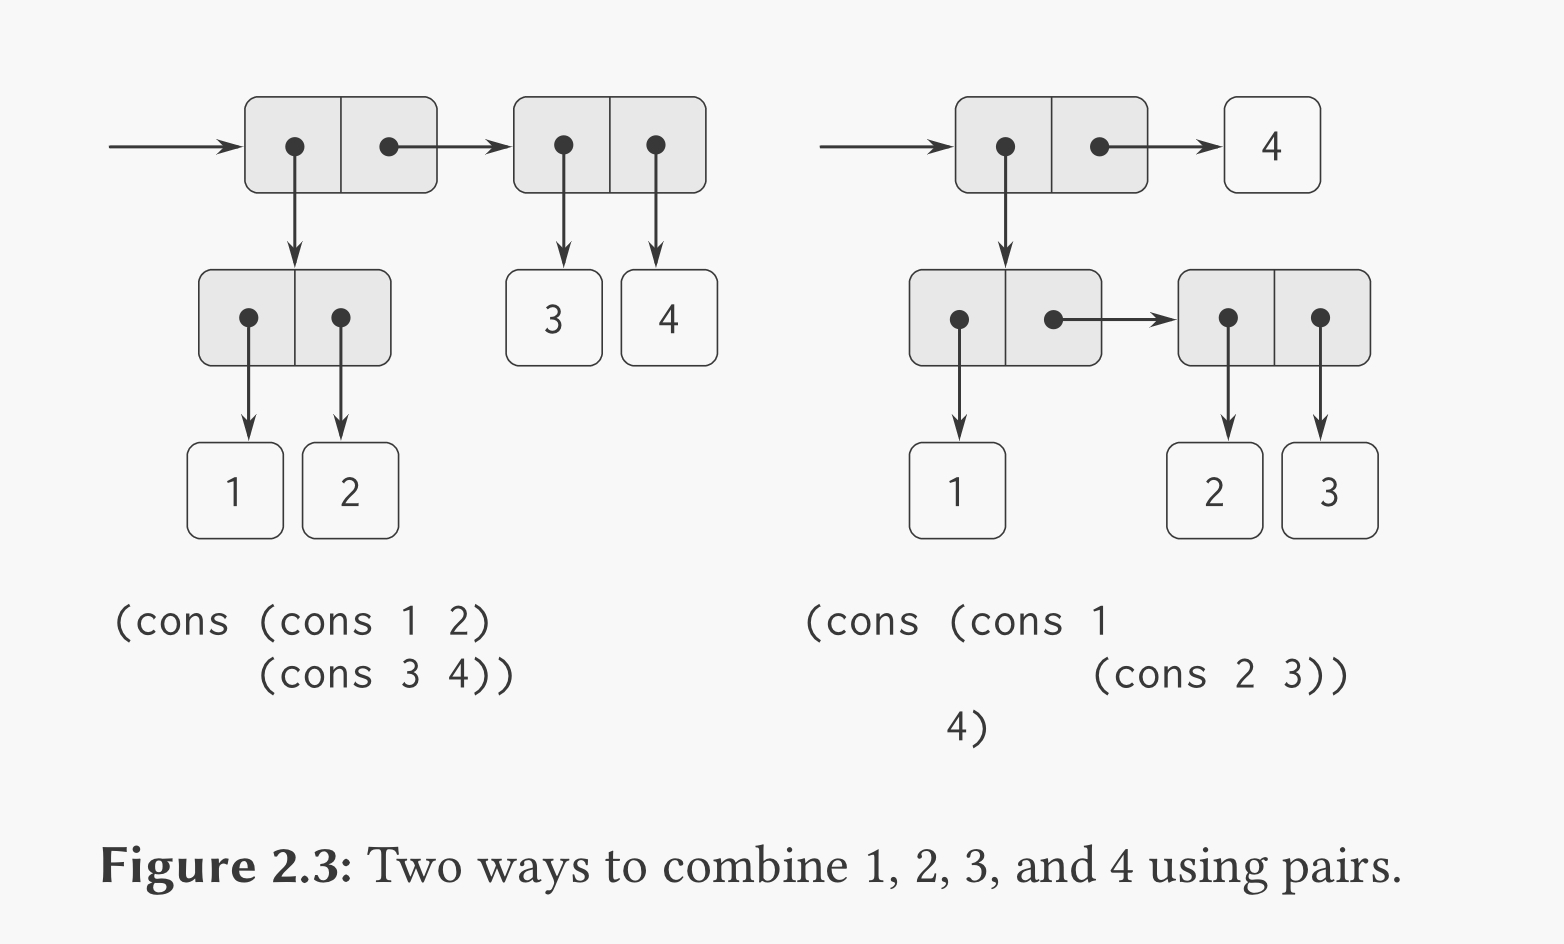
\includegraphics[width=.9\linewidth]{2/cons-cells.jpeg}
\end{center}

The ability to combine things using an operation, then combine those results
using the same operation, can be called the \textbf{closure property}. \texttt{cons} can
create pairs whose elements are pairs, which satisfies the closure property.
This property enables you to create hierarchical structures. We've already
regularly used the closure property in creating procedures composed of other
procedures.

\begin{quote}
\textbf{Definitions of ``closure''}

The use of the word ``closure'' here comes from abstract algebra, where a set of
elements is said to be closed under an operation if applying the operation to
elements in the set produces an element that is again an element of the set.
The Lisp community also (unfortunately) uses the word ``closure'' to describe a
totally unrelated concept: A closure is an implementation technique for
representing procedures with free variables. We do not use the word ``closure''
in this second sense in this book.
\end{quote}

\subsection{2.2.3: Sequences as Conventional Interfaces}
\label{sec:org9bd47b0}
Abstractions are an important part of making code clearer and more easy to
understand. One beneficial manner of abstraction is making available
conventional interfaces for working with compound data, such as \texttt{filter} and
\texttt{map}.

This allows for easily making ``signal-flow'' conceptions of processes:

\begin{center}
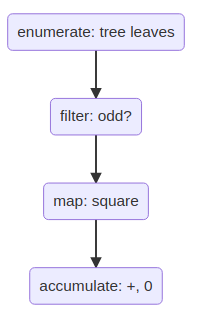
\includegraphics[width=0.3\linewidth]{2/fig/t_2-2-3.png}
\end{center}

\subsection{2.2.4: Example: A Picture Language}
\label{sec:org39dd6cf}
Authors describe a possible implementation of a ``picture language'' that tiles,
patterns, and warps images according to a specification. This language consists
of:

\begin{itemize}
\item a \textbf{painter} which makes an image within a specified parallelogram shaped
frame. This is the most primitive element.
\item \textbf{Operations} which make new painters from other painters. For example:
\begin{itemize}
\item \emph{beside} takes two painters, producing a new painter that puts one in the
left half and one in the right half.
\item \emph{flip-horiz} takes one painter and produces another to draw its image
right-to-left reversed. These are defined as Scheme procedures and therefore
have all the properties of Scheme procedures.
\end{itemize}
\end{itemize}
\end{document}
